\documentclass[english]{article}
\usepackage[T1]{fontenc}
\usepackage[latin9]{inputenc}
\usepackage{geometry}
\geometry{verbose,tmargin=3.5cm,bmargin=4cm,lmargin=3.8cm,rmargin=3.8cm}

\makeatletter
\usepackage{url}
\usepackage{lipsum}  
\usepackage{graphicx}  

\makeatother

\usepackage{babel}
\begin{document}

\title{
    
\includegraphics[width=8cm, keepaspectratio]{tudelftlogo.png}\\
    \vspace*{2cm}
    \textbf{
        Estimating the Amplification Factor of Three Common Protocols in DRDoS Attacks\\
        % {\large A Measurement Study on the Weaponisation of Hosts from Greece}
        {\large A Quantitative Analysis on the Weaponization of Hosts Located in Greece}
        % {\large Assessing the Amplification Potential of Servers from Greece}
    }\\
    \vspace*{1cm}
}

\author{
     \textbf{
Rares-Andrei Toader$^1$}\\
    \hfill \break
    \textbf{Supervisors: Georgios Smaragdakis$^1$, Harm Griffioen$^1$ }\\
    \break
%    \affiliations
    {\large 
        \hfill \break
        $^1$EEMCS, Delft University of Technology, The Netherlands
    }\\
}

\date{}

\maketitle
\thispagestyle{empty}

\let\clearpagebackup\clearpage
\renewcommand{\clearpage}{ }

\onecolumn

\vspace*{1.5cm}
\begin{center}
    A Thesis Submitted to EEMCS Faculty Delft University of Technology,\\
    In Partial Fulfilment of the Requirements\\
    For the Bachelor of Computer Science and Engineering\\
    \today
\end{center}

\vspace*{2cm}

\noindent
{\small
Name of the student: Rares-Andrei Toader \\
Final project course: CSE3000 Research Project\\
Thesis committee: Georgios Smaragdakis, Harm Griffioen, Georgios Iosifidis	
\\
}
\vfill

\begin{center}
    An electronic version of this thesis is available at http://repository.tudelft.nl/.
\end{center}

\twocolumn
\let\clearpage\clearpagebackup  
\clearpage
\setcounter{page}{1}

\onecolumn

% \begin{abstract}
Distributed reflection denial-of-service (DRDoS) attacks are a type of cyberattack where a malicious actor sends requests to public and open servers on behalf of the victim by spoofing their IP address. The traffic generated by the corresponding responses is directed towards the victim (whose IP address appeared as the source address of the initial packets), potentially exhausting their bandwidth. These attacks have kept becoming more powerful over the years. 

This thesis presents a measurement study of three well-known protocols, where we assess the amplification potential of hosts located in Greece running these protocols. We find that DNS remains the most vulnerable protocol to amplification; the top 250 hosts can cumulatively amplify the traffic by 32,000$\times$. Furthermore, we discover that the ``ANY'' query type and the improperly configured DNS extension (EDNS0) are two significant causes of DNS amplification. Lastly, we also find hosts vulnerable to looping attacks, a novel threat in the context of DDoS attacks. 

% The aim of this template is to make it more clear what is expected from you. 
% \textbf{It is by no means required to follow this exact same structure.}
% The abstract should be short and give the overall idea:
% what is the background, the research questions, what are your contributions, and what are the main conclusions.
% It should be readable as a stand-alone text (preferably no references to the paper or to outside literature).
\end{abstract}

% \section{Introduction}


% Malicious actors typically launch denial-of-service attacks to reduce the availability of Internet servers. 
\looseness=-1 A \textit{denial-of-service attack} (DoS) is a collection of cyber attacks that aim to disrupt the availability of a system~\cite{cloud_dos}. This attack and its variants have been widely researched~\cite{ddos_taxonomy} in the literature and have historically been one of the most popular strategies used by adversaries~\cite{crowdstrike_popular_attacks}. 

\looseness=-1 A \textit{distributed denial-of-service} (DDoS) attack has the same goal as a normal DoS attack~\cite{cloud_ddos}. However, it achieves this by having multiple adversarial entities exhausting the target's resources instead of a single attacking entity. DDoS is a more powerful attack than the normal DoS~\cite{cloud_ddos}. The attacking entities in a DDoS context could be compromised computers or infected IoT devices, which could be part of a larger, malicious entity called a \textit{botnet}~\cite{crowdstrike_botnet}. The target can be a web server or another network service. The flood of incoming packets or connection requests to the victim's system forces it to become slower, become unresponsive or even crash, denying regular service to legitimate users, thus violating the ``A'' (availability) from the CIA (Confidentiality, Integrity and Availability) triad~\cite{cia-triad}.

\looseness=-1 In a \textit{distributed reflection} DoS attack (DRDoS), a malicious actor uses public services to reflect traffic to a victim~\cite{amplification_hell}. The attacker sends requests on behalf of the victim, and in turn, the victim gets flooded with responses from the public services. Consequently, if enough requests are made and the size of the responses is large, the target's bandwidth is depleted. An amplification attack is essentially a DRDoS attack, where the attacker focuses on sending requesting packets to the public hosts, whose size would be smaller than the responding packets sent to the victim. In this sense, the response packets amplify the requesting packets, hence the attack's name. 

% IP Spoofing in UDP-based protocols makes it possible for an attacker to send packets on the victim's behalf. NEW

% The adversary must send packets on the victim's behalf to launch such an attack. This is possible due to IP spoofing in UDP-based protocols. OLD

\looseness=-1 Several reasons make amplification attacks possible. IP spoofing in UDP-based protocols makes it possible for an attacker to send packets on the victim's behalf. \textit{IP spoofing} means the attacker sets the source address in the IP header as the victim's IP address when sending a packet to a public server. Consequently, the victim receives the response packets from the servers. This happens because UDP-based protocols respond to queries without being required to establish a connection (which is the case for TCP-based protocols) and thus do not validate the IP address of the entity sending the request. IP spoofing is considered a bad practice, and measures for it have been described 24 years ago in an RFC (Request for Comments)~\cite{ferguson-2000}. This introduces the idea of network ingress filtering (commonly referred to as BCP38)~\cite{ferguson-2000}, which would be a general measure against denial-of-service attacks that utilise IP source address spoofing.  
However, empirical evidence shows that IP spoofing is an ongoing problem that has yet to be eliminated~\cite{spoofer_project}, remaining the most critical cause of amplification attacks~\cite{amplification_hell}.

\looseness=-1 Another essential cause for amplification attacks is an asymmetry between the size of a request to a public server and the size of the response. This asymmetry enables amplification and is a desirable feature for an attacker, as they only have to send a small packet to reflect a larger amount to the victim. This security issue is present in many protocols because these protocols have not been implemented with this aspect in mind. For example, the ``monlist'' command~\cite{cloud_monlist} allows users to query an NTP server, retrieving up to 600 hosts with which the NTP server has most recently communicated. This feature was mainly meant as a debugging tool but has also been weaponised by adversaries in successful DRDoS attacks~\cite{amplification_hell}.

\looseness=-1 The first DDoS attack happened in July 1999, more than 20 years ago~\cite{mit_first_ddos}. The biggest DDoS attack ever recorded took place in 2017~\cite{cloud_famoud_ddos}. It targeted Google services and peaked at 2.54 Tbps. DDoS attacks have kept getting more notoriety over the years, becoming well-established cyber attacks with a popularity that has kept rising. In a recent DDoS threat report for 2024 Q1, Cloudflare mentions that they have noticed a 50\% increase in DDoS attacks compared to the corresponding first quarter in 2023~\cite{cloud_q1report}. DDoS attacks are extremely popular in the cyber threat landscape for several reasons. Firstly, they are relatively easy to orchestrate, requiring little technical expertise, as they can even be bought online as a service, often under the umbrella name of ``stress-testing'', at a reasonable cost~\cite{buy_ddos}. Secondly, these attacks effectively overwhelm a victim's system, leading to downtime or service disruption. Moreover, the malicious actor can achieve this while also preserving their anonymity. 

\looseness=-1 Seeing the impact and complexity of DRDoS attacks, we realised there is no auditing tool to find servers in an autonomous system (AS)~\cite{autsys} that could be weaponised and, consequently, unintentionally participate in amplification attacks. The literature lacks a comprehensive list that enumerates all the negative aspects of all existing protocols or the configuration of a specific server that could contribute to launching an amplification attack.

\looseness=-1 As an extension, we also analyse looping attacks, a novel DoS attack at the application-layer level~\cite{cispa-loopy}. This particular attack leads to infinite amplification, as two vulnerable servers would send messages to each other indefinitely. This happens, for instance, when a host responds to a malformed request with an error message, and this response prompts another server to send the packet needed for the initial server to send the same error message. Thus, a traffic loop is formed between the two servers. This type of attack can be hazardous, as it could also be used to target network links. We follow the methodology in~\cite{cispa-loopy} to discover which servers are vulnerable and how many vulnerable host pairs could be formed. Note that our study focused on Greece, as this was the country assigned to us for our project. With this thesis, we make the following contributions:

\begin{itemize}[left=0pt, itemsep=0pt]
    \item We investigate which DNS, NTP, and Memcached servers located in Greece can be utilised in amplification attacks. 

    \item  We explore what amplification factor can typically be achieved with the Greek infrastructure explored and what conditions influence this factor. 

    \item We measure the number of vulnerable pairs of DNS and NTP servers located in Greece that could be formed in the context of looping attacks.
    
\end{itemize}



\looseness=-1 The thesis is structured as follows. In Section II, background information is given, such as definitions and important concepts. Section III mentions notable contributions related to our work. Section IV describes the data used in this work and how it was obtained. Section V presents the ways in which the experiments and measurements were performed. Section VI mentions the operational considerations enforced throughout this work in order to follow an ethical research procedure. Section VII highlights the results, and Section VIII showcases reflections on them. Lastly, Section VIII draws the conclusions. 







% \begin{itemize}
% \item Introduce the topic and explain why it is important (motivation!). %\emph{How should a scientific paper look like?}

% \item Relate to the most relevant existing work from the literature (use BibTeX), explain their contributions, and (critically) indicate what is still unanswered. 
% %\emph{The existing state of the art describes the setup of general scientific papers, e.g.\ see~\cite{hengl2002rules}, but this may be different for computer science papers.}

% \item Explain what the research questions for this work are. 
% This usually is a subset of the unanswered questions. %\emph{The aim of this work is therefore to provide a good template specifically for papers in the field of computer science.}

% \item Summarize the main contributions/conclusions of this research.
% NB: Make sure the title of the paper is a good match to the main research question / contribution / conclusion.

% \item Briefly indicate how the rest of the paper fits together to answer the research question(s).
% \end{itemize}

% For a longer research paper, a section with a more elaborate discussion of the literature may follow, but for short (conference) submissions, this is often included in the introduction.

% Make sure the introduction and conclusion are easily understandable by everyone with a computer science bachelor (e.g.\ your examiner may have a completely different expertise).

% \input{sections/methodology_or_problem_description}

% \input{sections/your_contribution}

% %\bigskip
% %\lipsum[1-67]

% \input{sections/experimental_setup_and_results}

% \section{Responsible Research}



\captionsetup{font=scriptsize}
\begin{table}[t]
    \raggedright % Aligns the table to the left
    \caption{BAF per protocol. ``All'' represents the mean BAF across all open amplifiers, 50\% and 10\% only consider the most vulnerable 50\% or 10\% of all open amplifiers. In the third column, in the NTP row, the first number shows the number of servers that responded to a Mode 3 request, and the second the hosts that responded to ``monlist''.}
    \scriptsize % Reduce font size (tiny is even smaller) /scriptsize
    \renewcommand{\arraystretch}{0.8} % Adjust row height
    \setlength{\tabcolsep}{1.3pt} % Adjust column spacing
    \begin{tabular}{lcccccc}
        \toprule
        \multirow{2}{*}{Protocol} & \multirow{2}{*}{\# of hosts} & \multirow{2}{*}{\# of open hosts} & \multicolumn{3}{c}{BAF} & \multirow{2}{*}{Strategy} \\
        \cmidrule(r){4-6}
         &  &  & All & 50\% & 10\% &  \\
        \midrule
        DNS & 7532 & 2398 & 16.5 & 33.1 & 128.5 & ``ANY'' on ``.sl'' \\
        DNS\(_{auth}\) & 926 & 926 & 11.8 & 18.4 & 26.0 & Max. ``ANY'' on own domains\\
        NTP & 25962 & 25129 / 632 & 2.8 & 4.7 & 19.1 & Max. of private queries\\
        Memcached & 13 & 0 & 0 & 0 & 0 & ``Get'' request \\
        \bottomrule
    \end{tabular}
    \label{tab:hosts_baf}
\end{table}

\looseness=-1 This section will present the considerations we made when conducting our experiments to follow an ethical research approach. 

\looseness=-1 \textbf{Ethical Considerations}. When gathering initial information about hosts, we employed passive scanning to be as non-intrusive as possible. In contrast, if done without proper authorisation, active scanning could have been seen as malicious by the other parties. Furthermore, in the filtering and measurement stage of our methodology, described in Section \RNum{5}, we send packets to a host once, and we set a cool-down period of 100 milliseconds between requests to prevent flooding the target with requests, as well as not exhausting the bandwidth of any network links, respectively. 

\looseness=-1 We will also make sure not to publish the IP addresses of hosts that are amplifiers to avoid the possibility of an attacker using this information and launching a DDoS attack. We wish to refrain from facilitating anyone with the resources to carry out such an attack. 
 

\looseness=-1 \textbf{Reproducibility}. Due to the dynamic character of the world's networks, it is impossible to guarantee the complete reproducibility of our experiments. For instance, due to IP address churn, the hosts we gathered might have different IPs if collected at different times in the future~\cite{griffioen_quantifying_2020}. Similarly, the vantage point from which the experiments are conducted might influence the results~\cite{wagner_united_2021}. Nonetheless, we have created a Dockerfile that specifies everything one needs to run our experiments in the same setting (i.e., the same dependencies and versions). The scripts are also open-source and hosted on the author's GitHub~\cite{rares_code}. 


% \captionsetup{font=scriptsize}
% \begin{table}[t]
%     \raggedright % Aligns the table to the left
%     \caption{BAF per protocol. ``All'' represents the mean BAF across all open amplifiers, 50\% and 10\% only consider the most vulnerable 50\% or 10\% of all open amplifiers. In the third column, in the NTP row, the first number shows the number of servers that responded to a Mode 3 request, and the second the hosts that responded to ``monlist''.}
%     \scriptsize % Reduce font size (tiny is even smaller) /scriptsize
%     \renewcommand{\arraystretch}{0.8} % Adjust row height
%     \setlength{\tabcolsep}{1.3pt} % Adjust column spacing
%     \begin{tabular}{lcccccc}
%         \toprule
%         \multirow{2}{*}{Protocol} & \multirow{2}{*}{\# of hosts} & \multirow{2}{*}{\# of open hosts} & \multicolumn{3}{c}{BAF} & \multirow{2}{*}{Strategy} \\
%         \cmidrule(r){4-6}
%          &  &  & All & 50\% & 10\% &  \\
%         \midrule
%         DNS & 7532 & 2398 & 16.5 & 33.1 & 128.5 & ``ANY'' on ``.sl'' \\
%         DNS\(_{auth}\) & 926 & 926 & 11.8 & 18.4 & 26.0 & Max. ``ANY'' on own domains\\
%         NTP & 25962 & 25129 / 632 & 2.8 & 4.7 & 19.1 & Max. of private queries\\
%         Memcached & 13 & 0 & 0 & 0 & 0 & ``Get'' request \\
%         \bottomrule
%     \end{tabular}
%     \label{tab:hosts_baf}
% \end{table}


% Reflect on the ethical aspects of your research and discuss the reproducibility of your methods.
% Note that although in many published works there is no such a section (it may be part of some meta-information collected by the journal, or part of the discussion section), we require you to think (and report) about this as part of this course.

% \section{Discussion}

\looseness=-1 We have noticed that ``ANY'' and the EDNS0 buffer size of 4,096 are the main culprits of DNS amplification attacks. We have not found significant amplification potential for NTP and Memcached, likely due to effective patching campaigns held in the past~\cite{exit_hell}. This does not imply that these protocols are not dangerous around the world. Thus, we still recommend patching NTP to turn off private queries (which is the case for ``ntpd'' versions of 4.2.8 and above~\cite{ntpd-patched}) and for Memcached to disable the UDP port by default~\cite{memcached-fixed}, by upgrading the vulnerable version to version ``1.5.6'' or above~\cite{memcached-fixed-version}.

\looseness=-1 \textbf{Peer outcomes}. The influence of the EDNS0 buffer size on BAF in the context of DNS amplification spans other countries as well, namely Belgium (BE), Luxembourg (LU), France (FR), Sweden (SE) and the Netherlands (NL). However, the distribution of which values for the buffer size are advertised differs from country to country; for instance, hosts located in NL choose a size of 1,232 way more often than a value larger than 4k (almost $5\times$ more often), showing a better adoption of the measures suggested by~\cite{dnsflagday}. In our case, a value larger than 4k was advertised more than $6\times$ compared to 1,232. We also see 1,232 being advertised in the majority of cases in FR. The BAFs we found for DNS are similar to the ones observed in BE, LU and SE. Moreover, recursive NS are more easily weaponizable in these countries than authoritative NS. When analysing NTP and Memcached amplification, FR and NL are more vulnerable than any other country from our peers, with hosts that run these protocols and lead to high BAFs. For FR, we conclude that this might be the case due to the sheer number of hosts, the likelihood of finding exploitable hosts being thus larger. Lastly, BE, FR, and SE also showcase the Linux NTP servers, which leads to large BAFs via Mode 7 queries.


\looseness=-1 We found similar results to what others have discovered in previous work~\cite{van_rijswijk-deij_dnssec_2014}; they observed that the majority of hosts that adopted EDNS0 advertise a buffer size of at least 4,000 bytes, namely in 70\% of our hosts. We noted the tendency for the BAF to increase as the buffer size becomes larger. Another interesting finding was that we even received larger responses than the advertised buffer size, which should not be the norm. As RFC9210~\cite{rfc9210} describes, when the data does not fit within the buffer size, the responding server should set the truncated flag to true in its response, and the requesting server should retry over TCP. Thus, the size of the answer should not exceed the buffer size. We concluded that two DNS implementations, MikroTik DNS and Raiden DNSD, set a default buffer size value of 4,096. Hosts running these two also got the highest BAFs out of all our DNS hosts, making up 70\% out of the top 250 of our hosts. Reflecting on our DNS results, we want to highlight that BAFs between 120 and 130 are readily achievable by attackers since relevant sources cite smaller values for DNS amplification. For instance, RFC5358~\cite{rfc-5358} states that values of 80 can be achieved, and CISA (Cybersecurity and Infrastructure Agency) mentions DNS can reach values between 28 and 54. The traffic that the top DNS hosts can generate can be destructive; an attacker capable of generating 100 megabits/second in queries can generate traffic as high as 3.89 terabits/second at the victim, as showcased by Table~\ref{tab:data}. This puts the DNS amplification provided by the top hosts located in Greece in a class of its own compared to the impactful Memcached attack from 2018, which reached a peak traffic of 1.3 Tbps~\cite{akamai2018attackspotlight}.  


\textbf{Mitigations}. As effective campaigns performed in the past managed to mitigate the dangers of NTP~\cite{exit_hell} and Memcached~\cite{akamai2018attackspotlight}, we hope that the cybersecurity community will continue to hold similar initiatives for DNS. We propose restricting the use of ``ANY'' queries as they are bound to lead to high amplification, which has also been suggested by an RFC~\cite{rfc-8482}. Even if extensive records need to be sent, we advise following the DNS flag day 2020 recommendation of setting the EDNS0 buffer size to 1,232 and adequately configuring it to send larger responses over TCP. Finally, we want to encourage every ISP to implement BCP38~\cite{ferguson-2000} to fight IP spoofing, which would lead to the extinction of spoof-based attacks. 

\textbf{Limitations}. Our work has only explored three protocols, but many other protocols that could be exploited exist (such as CharGen or SNMP~\cite{amplification_hell}). Furthermore, our results should serve as a lower bound to what an attacker could achieve in reality, as an attacker might further optimise and achieve a higher BAF for hosts than we achieved a small one. We have also only analysed the IPv4 range, as there were no IPv6 hosts on Censys running one of the studied protocols. Still, we want to highlight the need for further studies for IPv6 hosts. Lastly, a worldwide study would have to be conducted to confirm or contradict patterns found in our work, such as the influence of the EDNS0 buffer size.  


% \section{Conclusion}

\captionsetup{font=normalsize}
\begin{table}[t]
    \centering
    \caption{Theoretical amplification traffic when the attacker has an uplink of 100 Mbps.}
    \normalsize
    \begin{tabular}{cccc}
    \toprule
    \# of top hosts & Cumulative BAF & Victim (bits/s) \\
    \midrule
    100 & 13,073.35 & 1.307 T \\
    250 & 32,087.23 & 3.208 T \\
    500 & 38,964.94 & 3.8964 T \\
    \bottomrule
    \end{tabular}
\label{tab:data}
\end{table}

\looseness=-1 \textbf{Summary}. We have analysed the amplification potential of three protocols from hosts located in Greece. We have shown that DNS remains a very effective amplification vector; the cumulative BAF provided by the worst $250$ DNS amplifiers was $\approx 32,000$. We have determined that ``ANY'' queries and a large EDNS0 buffer size lead to high DNS amplification. Moreover, two popular DNS implementations (Raiden DNSD and MikroTik) set a default value of 4,096 for the buffer size. In contrast, we have not found significant amplification potential in NTP and Memcached hosts (located in Greece). Lastly, we discovered that looping attacks are also possible among the hosts considered. We found some vulnerable same protocol server pairs, leading to $7$ potential loops. 


\looseness=-1 \textbf{Future Work}: We would like to raise awareness of the dangers of DRDoS attacks and the need for further research. While our measurement study focused on three protocols, numerous other protocols (e.g. CharGen, SNMP) could be exploited. Future research should expand to include these and potentially other protocols to provide a more comprehensive understanding of amplification threats. This should be done in the context of an extensive and diverse dataset with better geographic coverage to ensure that the findings are globally representative and account for regional differences in network configurations and security practices. Since our results are a lower bound of what attackers can accomplish in practice, we believe studying amplifiers and real DRDoS attacks could give invaluable insights into how protocols are exploited (i.e. how an attacker optimises to reach the highest BAF). Last but not least, our analysis was limited to the IPv4 range. Further research should focus on identifying and analysing IPv6 hosts running protocols that can lead to amplification to understand this risk in the IPv6 space. This is crucial as the adoption of IPv6 continues to grow.

\clearpage





% % \newpage
% \onecolumn

\appendices

\section{Censys queries}
\label{appendix:censys_queries}

The queries used to retrieve hosts from Censys are shown below. One command was used for each protocol. Note that the number of pages used was large enough to fetch all hosts from Censys. Alternatively, one could set the ``pages'' flag to $-1 $ to retrieve all the pages.

% \lstset{
%   language=bash, 
%   basicstyle=\ttfamily\small,
%   keywordstyle=\color{blue},
%   commentstyle=\color{gray},
%   stringstyle=\color{black},
%   numbers=left,
%   numberstyle=\tiny\color{gray},
%   stepnumber=1,
%   numbersep=5pt,
%   backgroundcolor=\color{white},
%   frame=single,
%   breaklines=true,
%   breakatwhitespace=false,
%   showspaces=false,
%   showstringspaces=false,
% }

\definecolor{mygreen}{rgb}{0,0.6,0}
\definecolor{mygray}{rgb}{0.5,0.5,0.5}
\definecolor{myblue}{rgb}{0,0,0.8}
\definecolor{myorange}{rgb}{0.8,0.4,0}

% Define style for shell scripts
\lstdefinestyle{shellstyle}{
    backgroundcolor=\color{white},   
    commentstyle=\color{mygreen},
    keywordstyle=\color{myblue},
    numberstyle=\tiny\color{mygray},
    stringstyle=\color{myorange},
    basicstyle=\ttfamily\footnotesize,
    breakatwhitespace=false,         
    breaklines=true,                 
    captionpos=b,                    
    keepspaces=true,                 
    numbers=left,                    
    numbersep=5pt,                  
    showspaces=false,                
    showstringspaces=false,
    showtabs=false,                  
    tabsize=2,
    language=bash
}

% Define colors for syntax highlighting
\definecolor{mygreen}{rgb}{0,0.6,0}
\definecolor{mygray}{rgb}{0.5,0.5,0.5}
\definecolor{mymauve}{rgb}{0.58,0,0.82}
\definecolor{myblue}{rgb}{0,0,0.8}

% Define style for Python listings
\lstdefinestyle{pythonstyle}{
    backgroundcolor=\color{white},   
    commentstyle=\color{mygreen},
    keywordstyle=\color{myblue},
    numberstyle=\tiny\color{mygray},
    stringstyle=\color{mymauve},
    basicstyle=\ttfamily\footnotesize,
    breakatwhitespace=false,         
    breaklines=true,                 
    captionpos=b,                    
    keepspaces=true,                 
    numbers=left,                    
    numbersep=5pt,                  
    showspaces=false,                
    showstringspaces=false,
    showtabs=false,                  
    tabsize=2,
    language=Python
}

% % Apply the style to Python listings
% \lstset{style=pythonstyle}

% Apply the style to shell listings
\lstset{style=shellstyle}

\begin{itemize}
\item DNS:
\begin{lstlisting}[language=bash, caption=DNS query., label=lst:censys_dns]
censys search 'services.service_name: DNS and services.port:53 and 
location.country: "Greece"' --per-page 100 --pages 77 > dns.json
\end{lstlisting}
\item NTP:
\begin{lstlisting}[language=bash, caption=NTP query., label=lst:censys_ntp]
censys search 'services.service_name: NTP and services.port:123 and 
location.country: "Greece"' --per-page 100 --pages 267 > ntp.json 
\end{lstlisting}
\item Memcached:
\begin{lstlisting}[language=bash, caption=Memcached query., label=lst:censys_memcached]
censys search 'services.service_name: MEMCACHED and services.port:11211 and  
location.country: "Greece"' --per-page 100 --pages 1 > memcached.json
\end{lstlisting}

\end{itemize}




\section{Filter queries}
\label{appendix:filter_queries}

After gathering our hosts, we send simple queries to each one to see whether or not they are open to the public in our so-called ``filtering'' stage. Each query strategy (i.e. hand-crafted packet) is shown below. For DNS, we send a simple ``A'' query to resolve the IP address of google.com, as demonstrated in Listing~\ref{lst:check_dns}. When filtering NTP hosts, we first send a normal Mode 3 (client) request that can be seen in Listing~\ref{lst:check_ntp_1} and then send a ``monlist'' packet to the servers that responded to the previous query, as shown in Listing~\ref{lst:check_ntp_2}. We send a ``stats slabs'' request for Memcached hosts to filter them, as shown in Listing~\ref{lst:check_memcached}.

\lstset{style=pythonstyle}

\begin{itemize}
\item DNS:
\begin{lstlisting}[language=python, caption=DNS ``A'' request., label=lst:check_dns]
pkt = IP(dst=ip) / UDP(dport=53, sport=RandShort()) / DNS(rd=1, qd=DNSQR(qname="google.com"))
\end{lstlisting}
\item NTP:
\begin{lstlisting}[language=python, caption=NTP request., label=lst:check_ntp_1]
pkt = IP(dst=ip) / UDP(dport=123, sport=RandShort()) / NTP(version=4, mode=3)
\end{lstlisting}
\begin{lstlisting}[language=python, caption=NTP ``monlist'' query., label=lst:check_ntp_2]
data = "\x17\x00\x03\x2a" + "\x00" * 4  
# 0x17 for private mode, 0x00 for response, 0x03 for version, 0x2a for monlist
pkt = (IP(dst=ip) / UDP(dport=123, sport=RandShort()) / Raw(load=data)) 
\end{lstlisting}
\item Memcached:
\begin{lstlisting}[language=python, caption=Memcached ``stats slabs'' request., label=lst:check_memcached]
pkt = IP(dst=ip) / UDP(sport=RandShort(), dport=11211) / Raw(load="\x00\x01\x00\x00\x00\x01\x00\x00stats slabs\r\n")
\end{lstlisting}

\end{itemize}




\section{Measurement queries}
\label{appendix:measurement_queries}

To measure the BAF for the protocols, we have hand-crafted different packets that will lead to high amplification. In the case of DNS, we send an ``ANY'' request to the ``.sl'' TLD, presented in Listing~\ref{lst:measure_dns}. Note from the code that the request can easily be changed to be a ``DNSKEY'' or ``RRSIG'' request by changing the ``query\_type'' accordingly. We have mostly tried ``ANY'' as it would lead to the highest amplification factor if the server responded to it. For NTP, we send a ``monlist'' request, which was presented in Listing~\ref{lst:check_ntp_2}, along with some other private Mode queries~\cite{rapid7_private}, that are shown in Listing~\ref{lst:measure_ntp_private}.  For Memcached, we need to send two initial queries to find information about the keys and values present in the server. Our first query is a ``stats items'' query (Listing~\ref{lst:measure_mem_1}). This command retrieves statistical information about the items stored in the cache, providing details about each slab class (a logical grouping of cache entries of similar size). We parse the output from this command to retrieve all slab IDs. We then send, for each slab ID, a ``stats cachedump'' request (Listing~\ref{lst:measure_mem_2}). The 0 in the request indicates no limit, i.e. the server should answer with all items. This query retrieves information about items stored in a specific slab class. Each entry (i.e. item) contains the key, the size of the associated value and a timestamp (when the item was last accessed or possibly when it was set, depending on the version and configuration). This is the information we were looking for as we look to find the key and value that would lead to the highest BAF for the request we are considering (i.e. ``get $<key>$''). The code for this request is shown in Listing~\ref{lst:measure_mem_3}.

We also wanted to analyse the maximum theoretical BAF for Memcached for the ``get $<key> <key> ... <key>$'' request. We created a function for the theoretical BAF, named $b$, shown in Equation~\eqref{eq:mem_baf}, where $k$ is the size of the key, $v$ is the size of the associated value, and $t$ is the number of times the key appears in the ``get'' request. As $t$ tends to infinity, the BAF becomes equal to $\frac{v}{k + 1}$, as shown in Equation~\ref{eq:limit}. In the ideal case, the key has the smallest size possible, one character (thus one byte), and the value the largest size possible, 1 MB (i.e. $10^6$ bytes). This means that the largest theoretical BAF for this request will tend to a value of $\frac{10^6}{1+1} =\frac{10^6}{2}=500k$. This should show that the size of the key and the value associated with it directly impact the BAF potential of Memcached. 


\begin{figure}[htpb]
    \footnotesize
    \begin{equation}
     b(k, v,t) = \frac{v \cdot t}{13 + t \cdot (k + 1)}
    \label{eq:mem_baf}
    \end{equation}
    
    \begin{equation}
    \lim_{t \to \infty} b(k, v, t) = \lim_{t \to \infty} \frac{v \cdot t}{13 + t \cdot (k + 1)} = \frac{v}{k + 1}
    \label{eq:limit}
    \end{equation}
\end{figure}

\begin{itemize}
\item DNS:
\begin{lstlisting}[language=python, caption=DNS ``ANY'' request on ``.sl''., label=lst:measure_dns]
dns = DNS(ad=1)
dns.qd = DNSQR(qname=domain, qtype=query_type, qclass="IN")  # query section
dns.ar = DNSRROPT(rclass=4096, z=1)  # additional records
request = IP(dst=ip) / UDP(dport=53, sport=RandShort()) / dns
\end{lstlisting}
\item NTP:
\begin{lstlisting}[language=python, caption=NTP private Mode requests., label=lst:measure_ntp_private]
packet = IP(dst=target_ip) / UDP(dport=123, sport=RandShort()) / NTPPrivate(
        response=0,  # i.e. this is a request
        more=0,  # not expecting multiple packets
        version=2,  # version number 2/3
        implementation=3,  # assuming XNTPD
        auth=0,  # no authentication
        mode=7,  # 6 => mode 6 (control) or mode 7 (private)
        seq=0,  # sequence number
        request_code=command_code, # 0 for PEER_LIST, 1 for PEER_LIST_SUM, 16 for GET_RESTRICT
        # mode 6 => 12 for CTL_OP_REQ_NONCE and 31 for UNSETTRAP
        err=0,
        nb_items=0,  # number of data items
        mbz=0,  # must be zero
        data_item_size=0,  # size of each data item
    )
\end{lstlisting}
\item Memcached:
\begin{lstlisting}[language=python, caption=Memcached ``stats items'' request., label=lst:measure_mem_1]
pkt = IP(dst=ip) / UDP(sport=RandShort(), dport=11211) / 
Raw(load="\x00\x01\x00\x00\x00\x01\x00\x00stats items\r\n")
\end{lstlisting}
\begin{lstlisting}[language=python, caption=Memcached ``stats cachedump'' request., label=lst:measure_mem_2]
pkt = IP(dst=ip) / UDP(sport=RandShort(), dport=11211) / 
Raw(load=f"\x00\x01\x00\x00\x00\x01\x00\x00stats cachedump {slab_id} 0\r\n")
\end{lstlisting}
\begin{lstlisting}[language=python, caption=Memcached ``get $<key>$'' request., label=lst:measure_mem_3]
pkt = IP(dst=ip) / UDP(sport=RandShort(), dport=11211) / 
Raw(load=f"\x00\x01\x00\x00\x00\x01\x00\x00get key\r\n")
\end{lstlisting}

\end{itemize}



% 48 DNSKEY
  



    % packet = IP(dst=target_ip) / UDP(dport=123, sport=RandShort()) / NTPPrivate(
    %     # rm_vn_mode=0x1B,
    %     response=0,  # This is a request
    %     more=0,  # Not expecting multiple packets
    %     version=2,  # Version number 2/3
    %     implementation=3,  # Assuming XNTPD
    %     auth=0,  # No authentication
    %     mode=7,  # 6 => mode 6 (control), or mode 7 (private)
    %     seq=0,  # Sequence number
    %     request_code=command_code,  # => 12 for CTL_OP_REQ_NONCE and 31 for UNSETTRAP
    %     err=0,
    %     nb_items=0,  # Number of data items
    %     mbz=0,  # Must be zero
    %     data_item_size=0,  # Size of each data item
    %     # data=(b'\x00' * 40)  # => ntpdc and ntpq add padding
        % )
\section{Collect metadata}
\label{appendix:collect_metadata}


To grasp the connection between certain factors and the BAF achieved by hosts, we had to augment our existing knowledge with some metadata. We had different procedures, the code of which is shown below. For DNS, we retrieved the product (e.g. RedHat) and vendor information (e.g. Enterprise Linux) from the JSON file already provided by Censys. To classify an NS as recursive or not, we used the code snippet in Listing~\ref{lst:check_recursive}, where we essentially try to resolve the IP of ``google.com'' by using a specific nameserver recursively by setting the recursive flag. Note that we also set a timeout of one second and do not consider a server to be recursive in case of an error or a timeout. To obtain authoritative name servers, we used the flipped approach. We don't use any nameserver, but for each Greek domain we gathered, we looked up its authoritative nameserver via the ``dig'' query shown in Listing~\ref{lst:ns_dig}. As a result, we get the authoritative NS domains, which we then map to IP addresses with a simple ``dig'' query, see Listing~\ref{lst:ns_find_ip}. Finally, we only keep the authoritative NS IP if it is located in Greece, which we check using the geolocation tool ``ipinfo''~\cite{ipinfo}; the code for this is shown in Listing~\ref{lst:ip_geoloc}. This outputs a JSON with various information, and we use the ``country'' attribute, which we match with ``GR''. 

We have obtained the DNS software run by hosts by using the ``fpdns'' command line utility tool~\cite{fpdns_kirei}. The code is presented in Listing~\ref{lst:fpdns_code}. We set a timeout of 20 seconds per each request. Note that ``fpdns'' is not a well-maintained tool and likely has trouble distinguishing between newer versions of DNS software. We count this as a limitation of our analysis.

For NTP, we have only gathered the system information (i.e. the operating system run by a host). We used the ``ntpq'' CLI utility tool, as described in~\cite{ntpq}. The code for this is shown in Listing~\ref{lst:ntpq_code}. We parse the output and retrieve the value for the ``system'' attribute. 

\lstset{style=shellstyle}

\begin{lstlisting}[language=bash, caption=Resolve the IP of google.com recursively, label=lst:check_recursive]
dig @<ip> google.com +rec +time=1
\end{lstlisting}


\begin{lstlisting}[language=bash, caption=Finds the authoritative nameservers of the placeholder domain. , label=lst:ns_dig]
dig <domain> NS +short
\end{lstlisting}


\begin{lstlisting}[language=bash, caption=Resolve the IP address of the authoritative nameserver domain. , label=lst:ns_find_ip]
dig +short <nameserver_domain>
\end{lstlisting}

\begin{lstlisting}[language=bash, caption=Find geolocation information about placeholder IP. , label=lst:ip_geoloc]
curl http://ipinfo.io/<ip_address>/json
\end{lstlisting}

\begin{lstlisting}[language=bash, caption=Find DNS software information about the placeholder host. , label=lst:fpdns_code]
fpdns -t 20 <ip_address>
\end{lstlisting}

\begin{lstlisting}[language=bash, caption=Find operating system ran by NTP host. , label=lst:ntpq_code]
ntpq -c rv <ip_address>
\end{lstlisting}


\begin{figure}[t]
    \centering
        \centering
        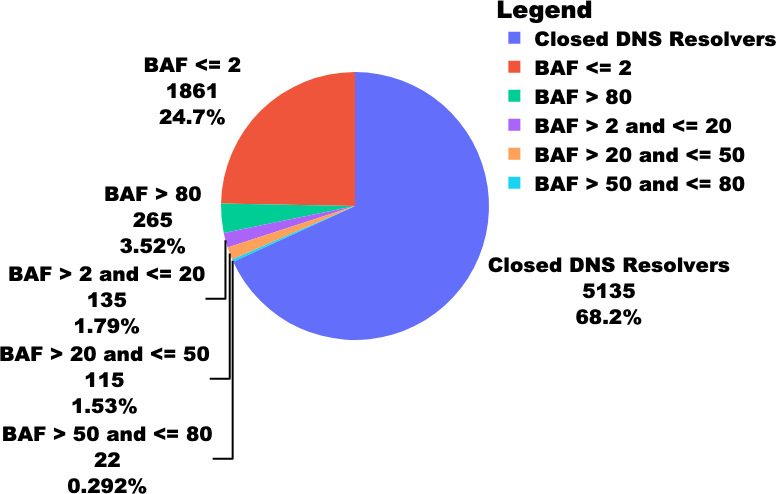
\includegraphics[width=0.48\textwidth]{research paper/plots/dns_sl_piechart_trim.png}
        \caption{DNS BAF distribution.}
        \label{fig:piechart_dns}
\end{figure}

\begin{figure}[t]
        \centering
        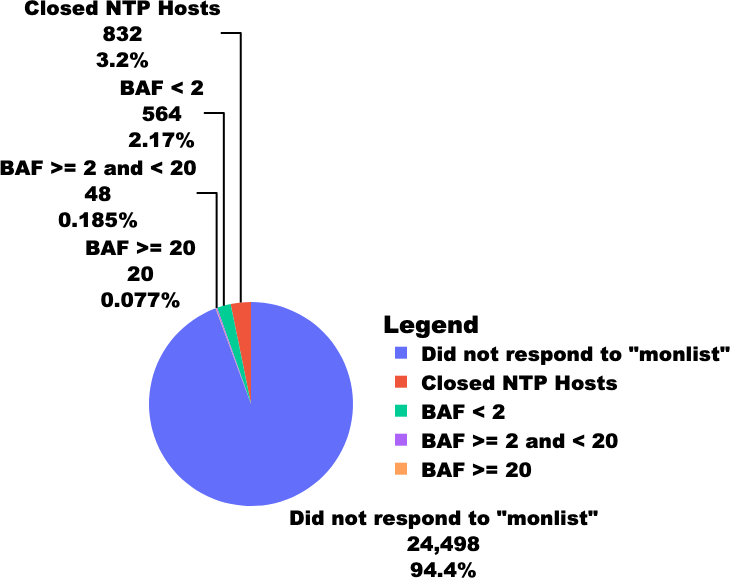
\includegraphics[width=0.48\textwidth]{research paper/plots/ntp_piechart_merged_trim.png}
        \caption{NTP BAF distribution.}
        \label{fig:piechart_ntp}
\end{figure}
    
\begin{figure}[t]
        \centering
        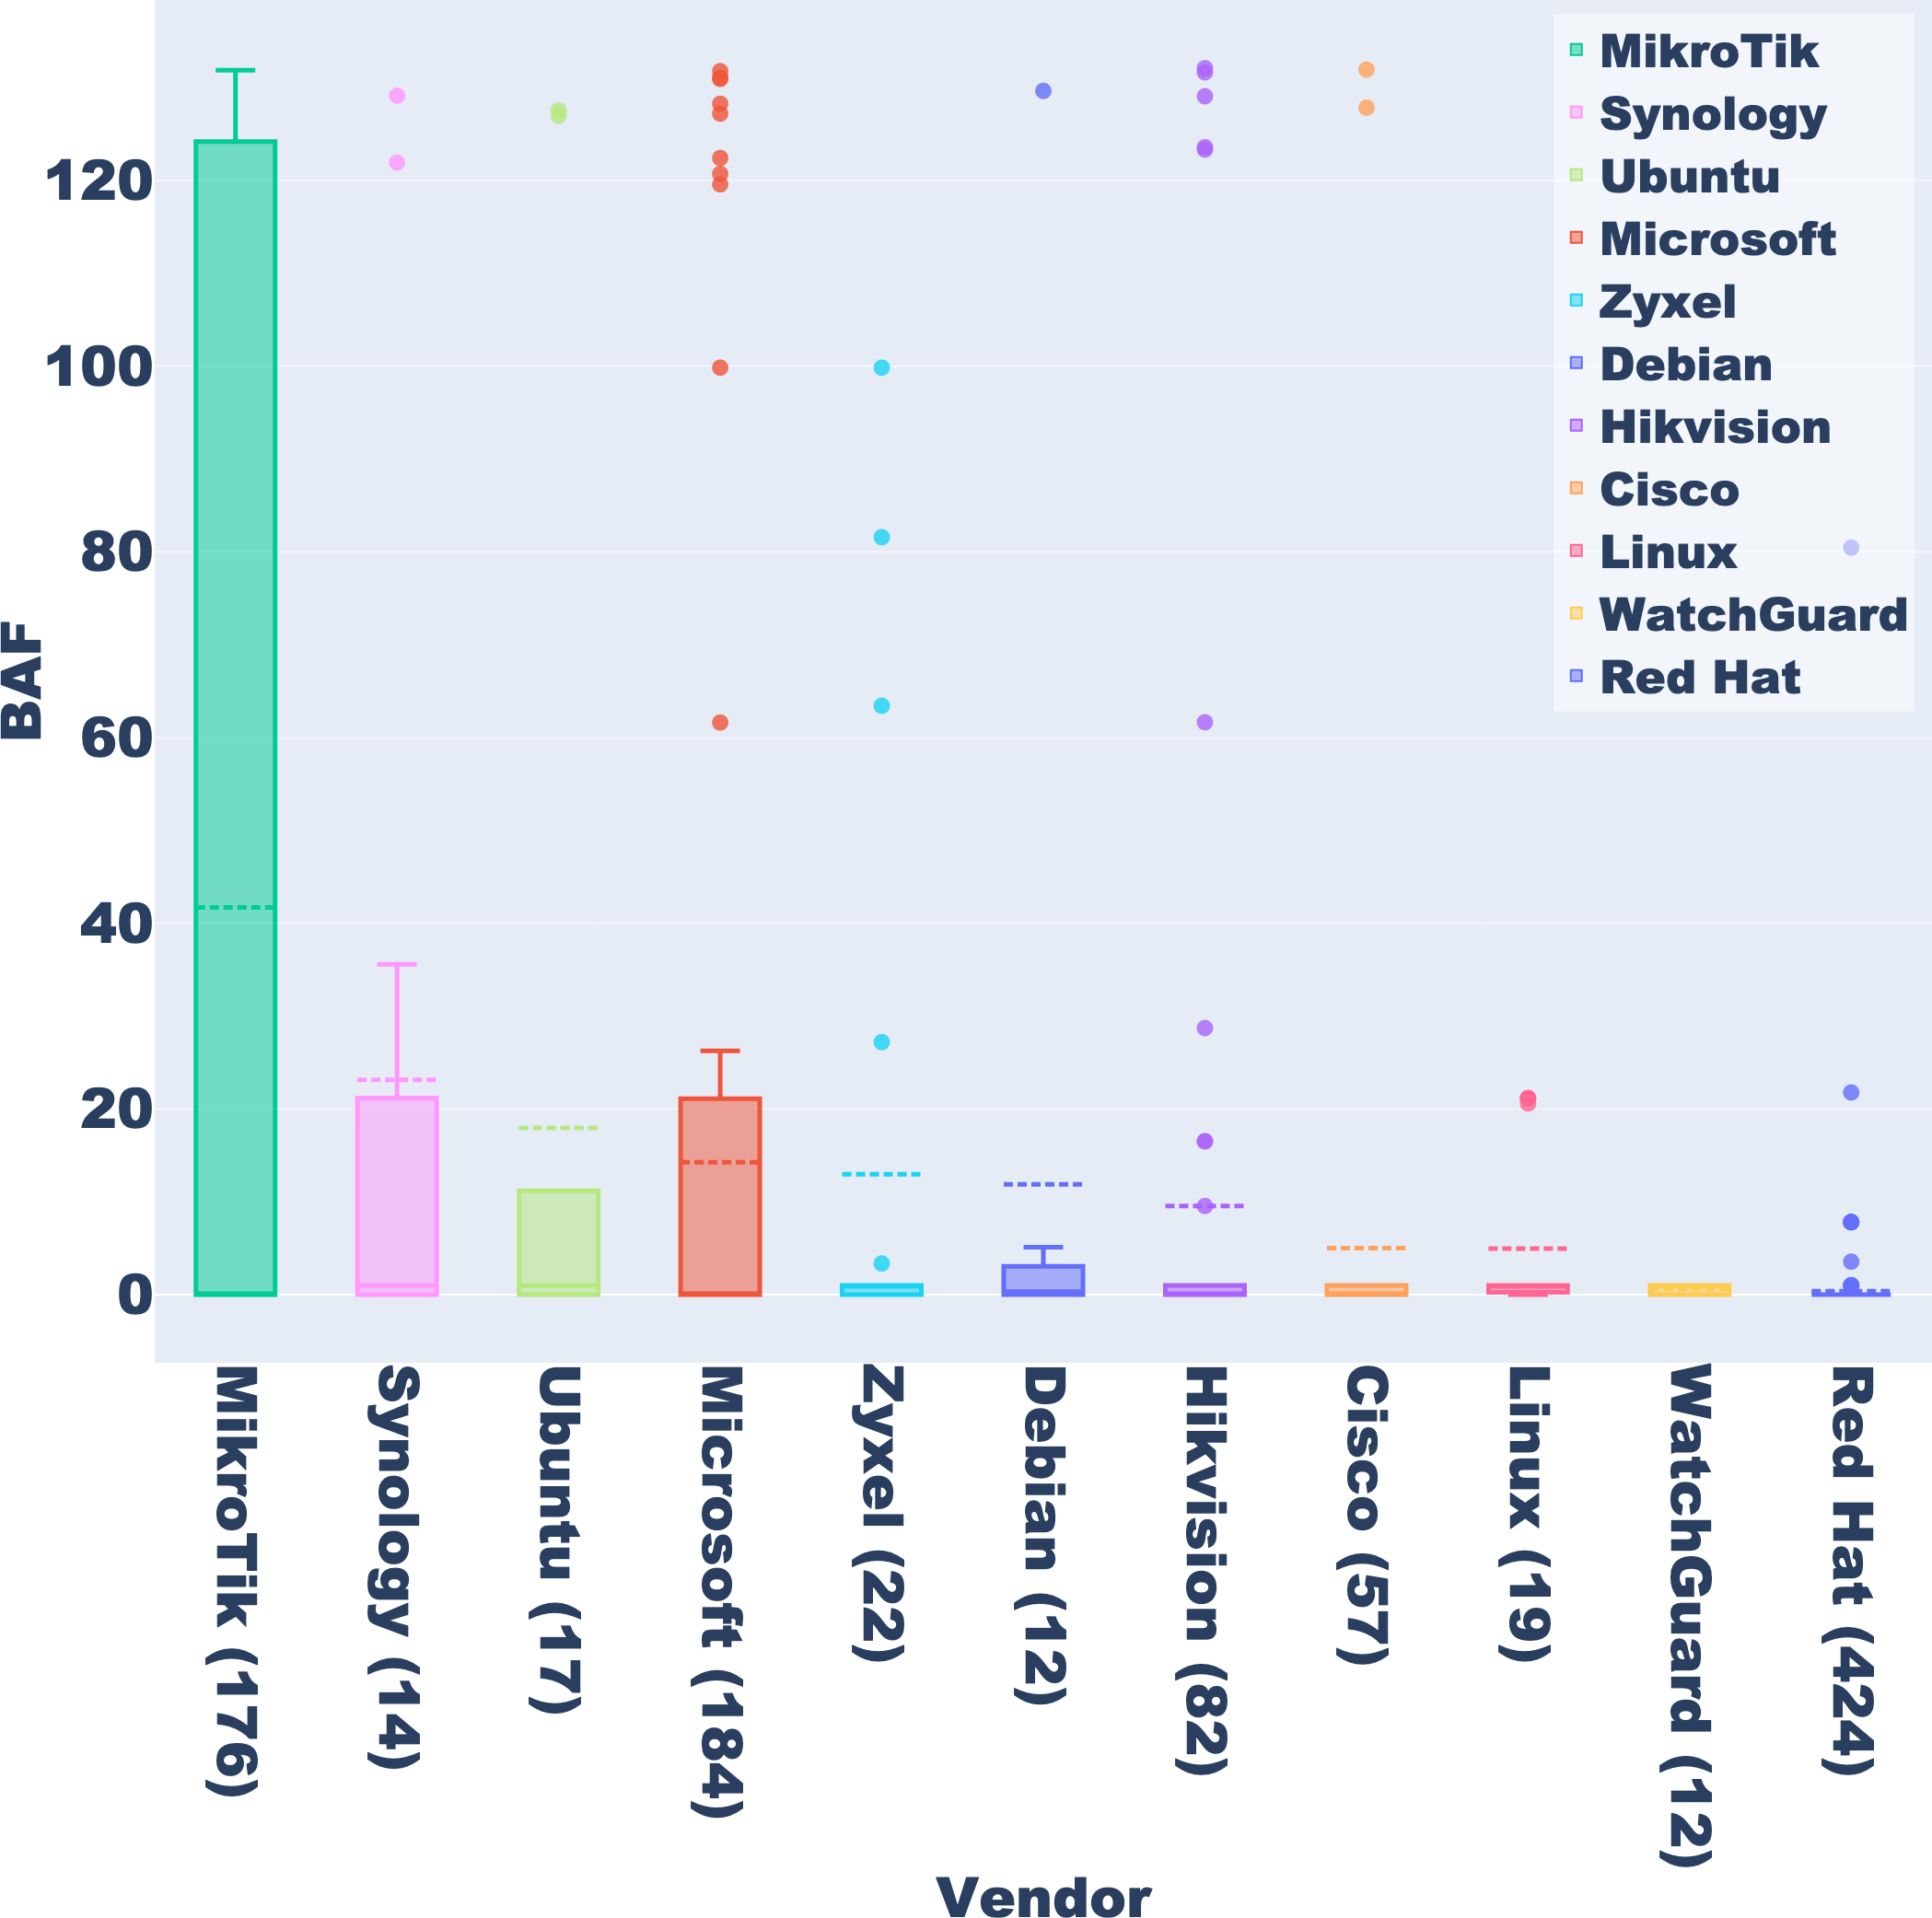
\includegraphics[width=0.48\textwidth]{research paper/plots/SL_vendor_boxplot_restricted_trim.png}
        \caption{Vendor against BAF (DNS).}
        \label{fig:boxplot_vendor}
\end{figure}
    
\begin{figure}[t]
        \centering
        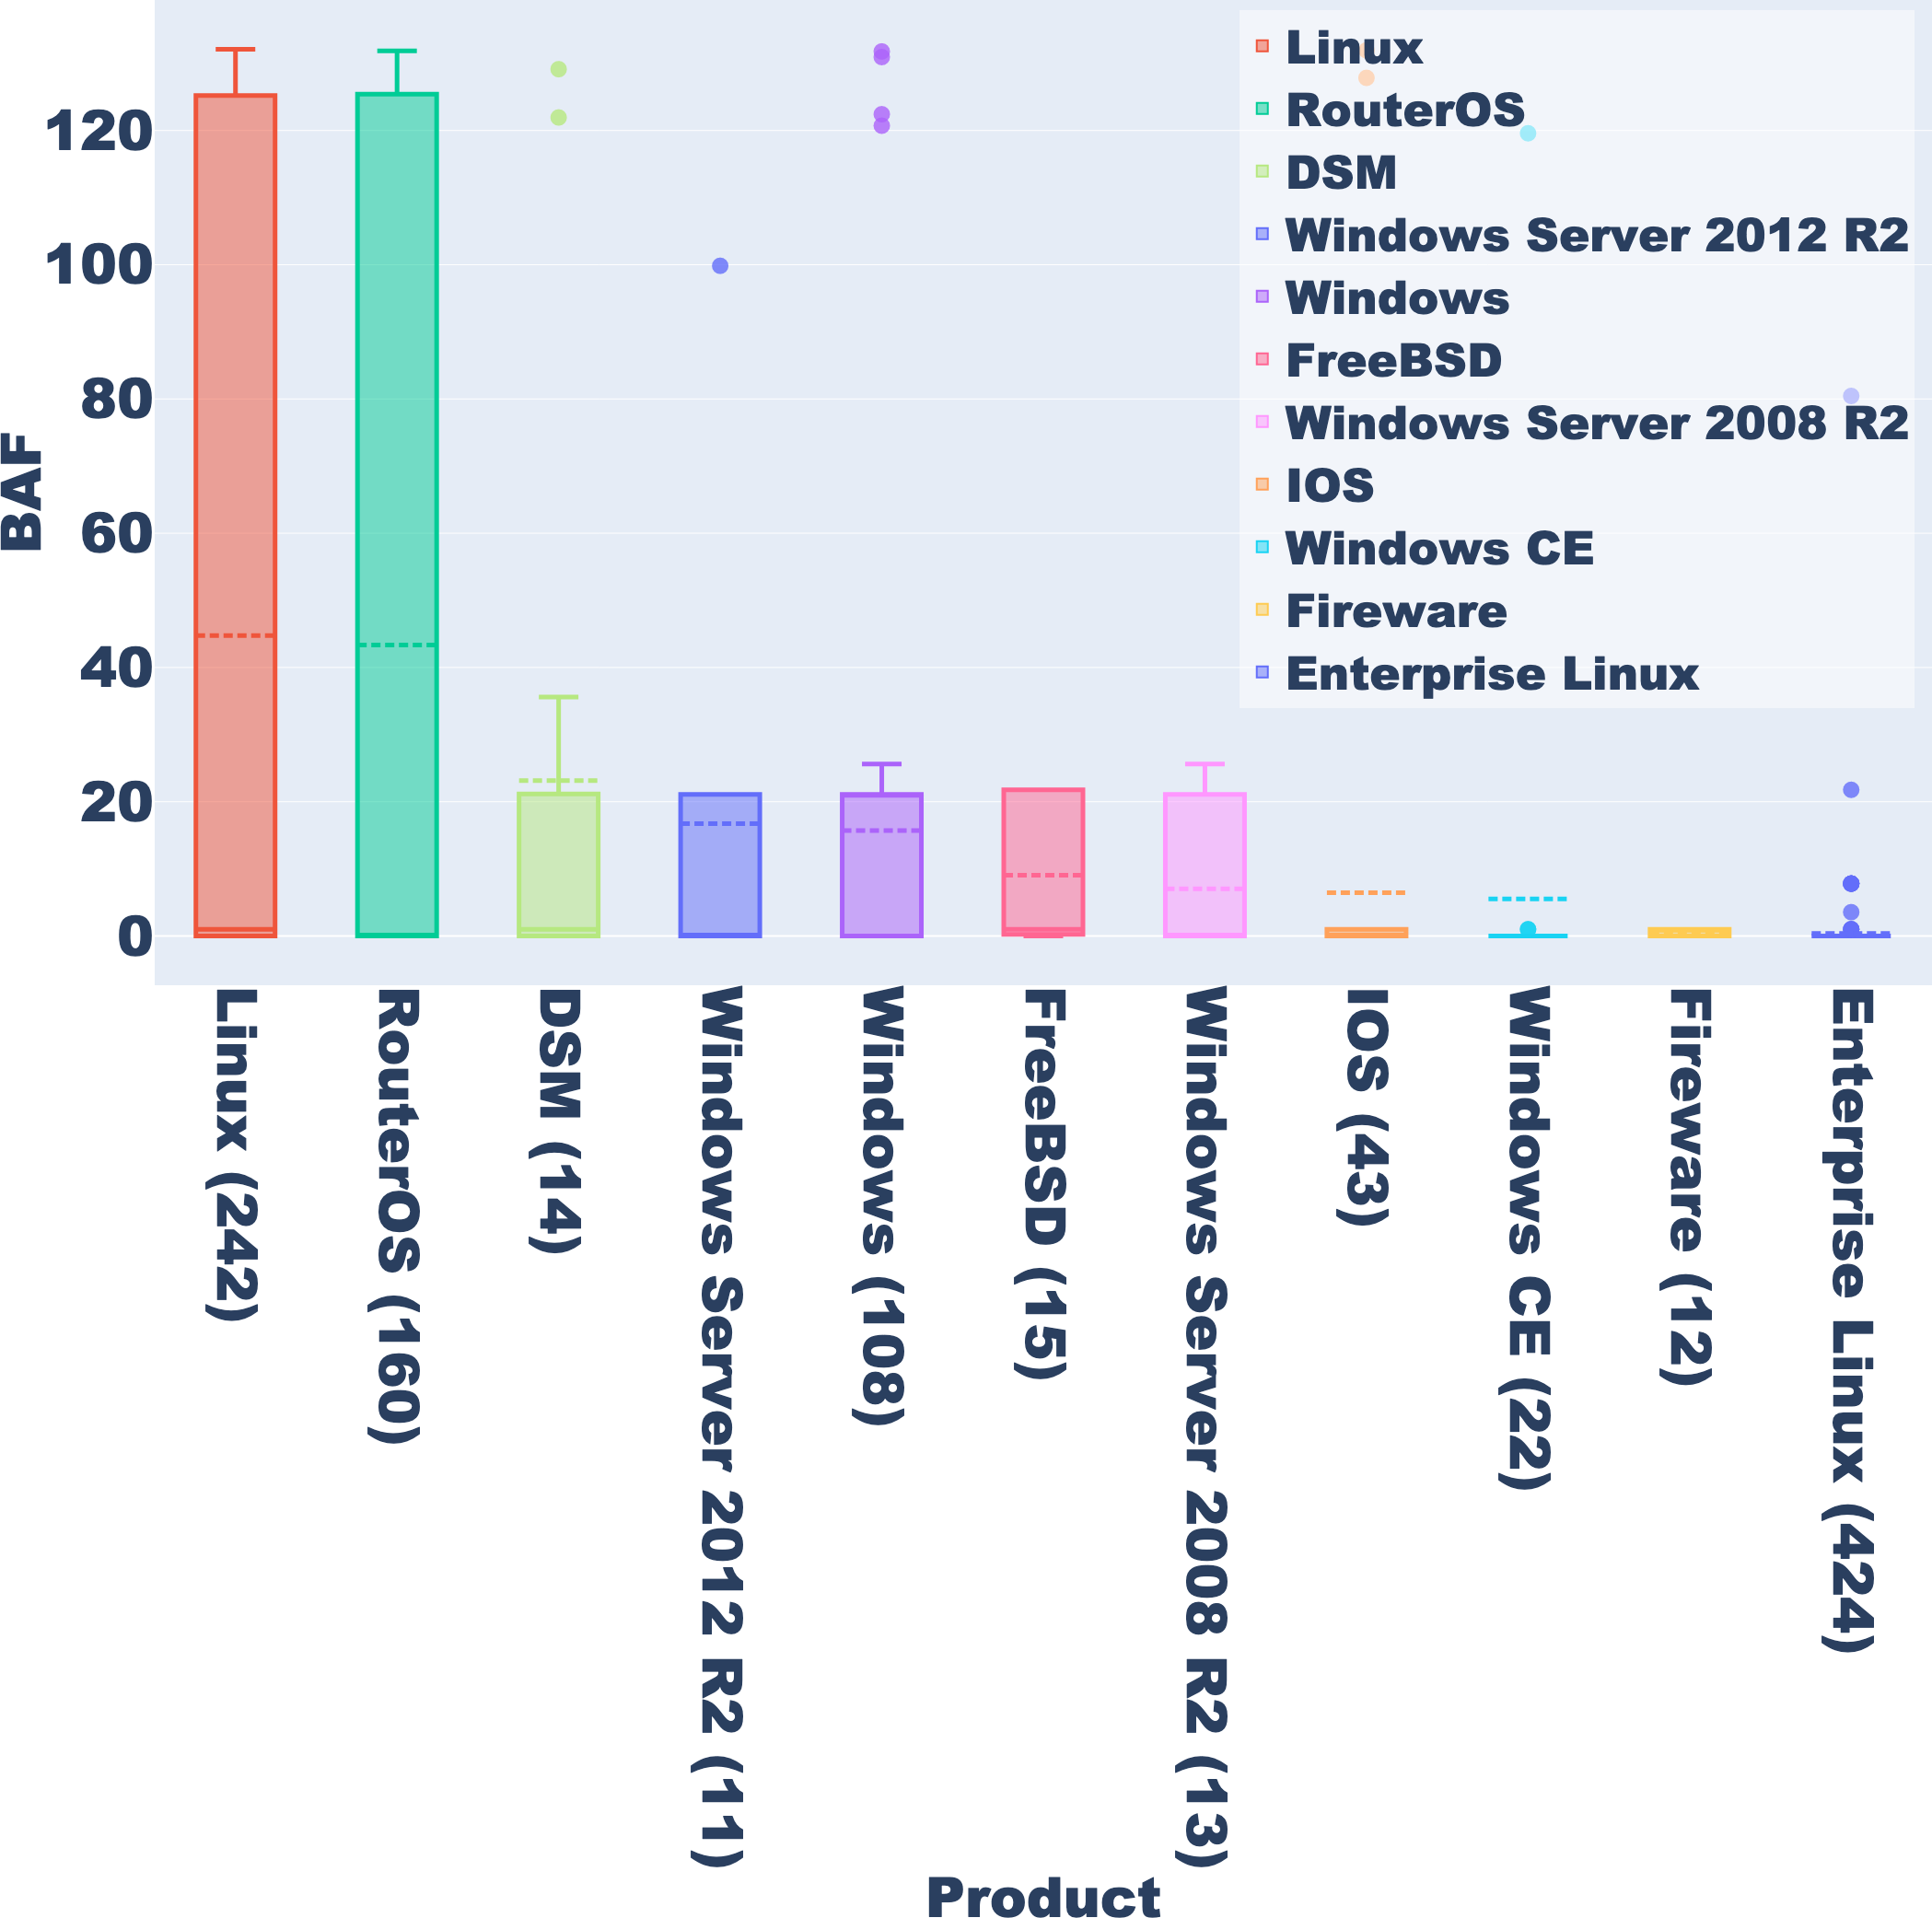
\includegraphics[width=0.48\textwidth]{research paper/plots/SL_product_boxplot_restricted_trim.png}
        \caption{Product against BAF (DNS).}
        \label{fig:boxplot_product}
\end{figure}
    % \caption{Piecharts for DNS and NTP and boxplots for DNS against product and vendor information.}
    % \label{fig:boxplots_piecharts}

\section{Piecharts and Boxplots}
\label{appendix:piecharts_boxplots}



The distribution of DNS hosts according to their BAF is shown in Fig.~\ref{fig:piechart_dns}. Most hosts are closed (68.2\%); however, quite a large amount of DNS hosts (265) achieve a BAF $\geq$ 80. A similar visualisation for NTP is shown in Fig.~\ref{fig:piechart_ntp}. Most NTP servers (94.4\%) did not respond to the ``monlist'' private Mode query for NTP. A few servers are closed (3.2\%), which was expected to ensure accurate and synchronised timekeeping across different devices and networks. Also, a tiny number (20) achieved a BAF $\geq 20$.  

The BAF distribution is depicted in a boxplot from the DNS hosts, whose vendor information we know, in Fig.~\ref{fig:boxplot_vendor}. Red Hat hosts are secure, almost all achieving a BAF of 0. In contrast, MikroTik servers reach the largest BAFs and some Microsoft and Hikvision outlier servers. Furthermore, the product (operating system) boxplot shown in Fig.~\ref{fig:boxplot_product} also shows that servers running RouterOS (from MikroTik) and Linux achieve the highest BAF. Unlike this, Enterprise Linux hosts (from Red Hat) are secure, achieving very small BAFs. Note that there is a high correlation between Fig.~\ref{fig:boxplot_vendor} and Fig.~\ref{fig:boxplot_product} in the sense that, for instance, all the RedHat hosts are running Enterprise Linux or all Synology hosts are running DSM~\cite{dsm}.


\section{Heatmaps}
\label{appendix:heatmaps}

The heatmaps from above compare pairs of factors, and each cell contains the median BAF attained per that respective group. The percentage of the feature on the x-axis is also displayed in parentheses. The total number of servers from certain features is displayed on the left and top borders for the y-axis and x-axis features. Fig.~\ref{fig:heatmap_version_product} shows that, interestingly, servers that get a high BAF that use the MikroTik implementation are not the ones that run Router OS as their operating system. The ones that obtain a high BAF are servers that run DSM (DiskStation Manager - from Synology) and Linux. Similarly, the groups that get the highest BAF in Fig.~\ref{fig:heatmap_buffer_product} are the ones that advertise a Buffer Size of 4,096.

\begin{figure}[t]
    \centering
    \begin{minipage}[t]{0.45\textwidth}
        \centering
        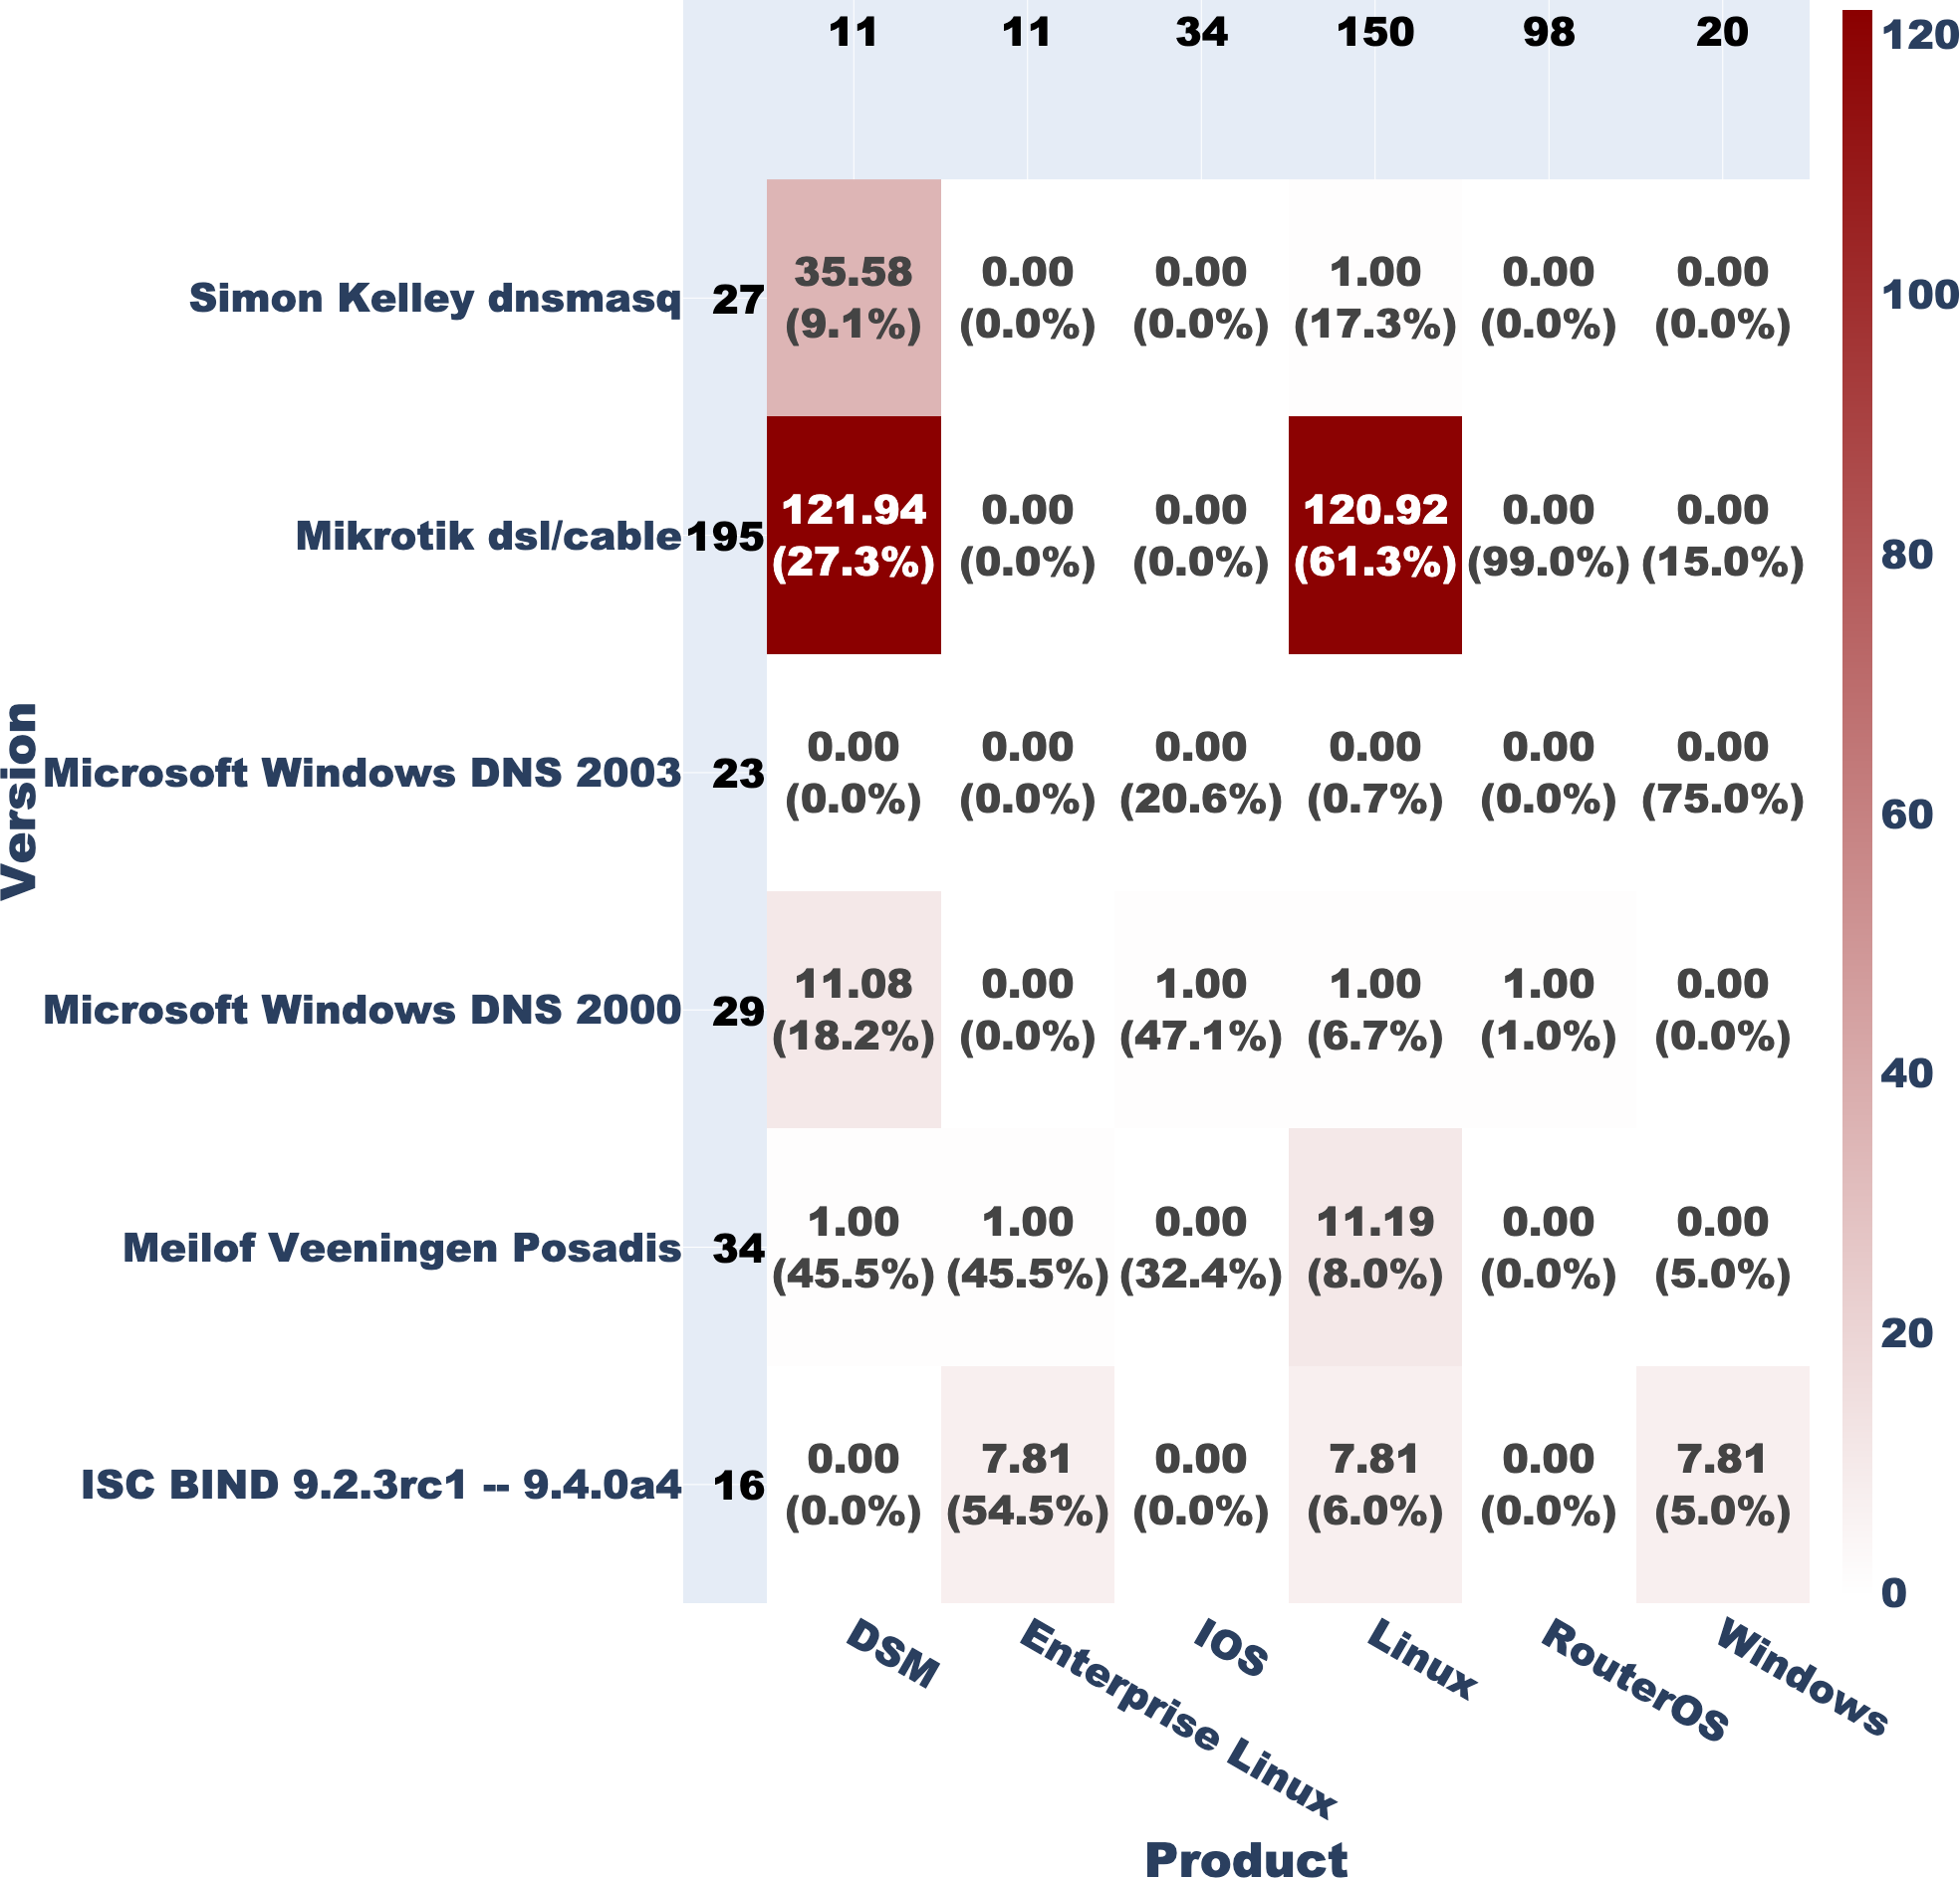
\includegraphics[width=\textwidth]{research paper/plots/filtered_Version_vs_Product_trim.png}
        \caption{Version against Product.}
        \label{fig:heatmap_version_product}
    \end{minipage}
    \hfill
    \begin{minipage}[t]{0.45\textwidth}
        \centering
        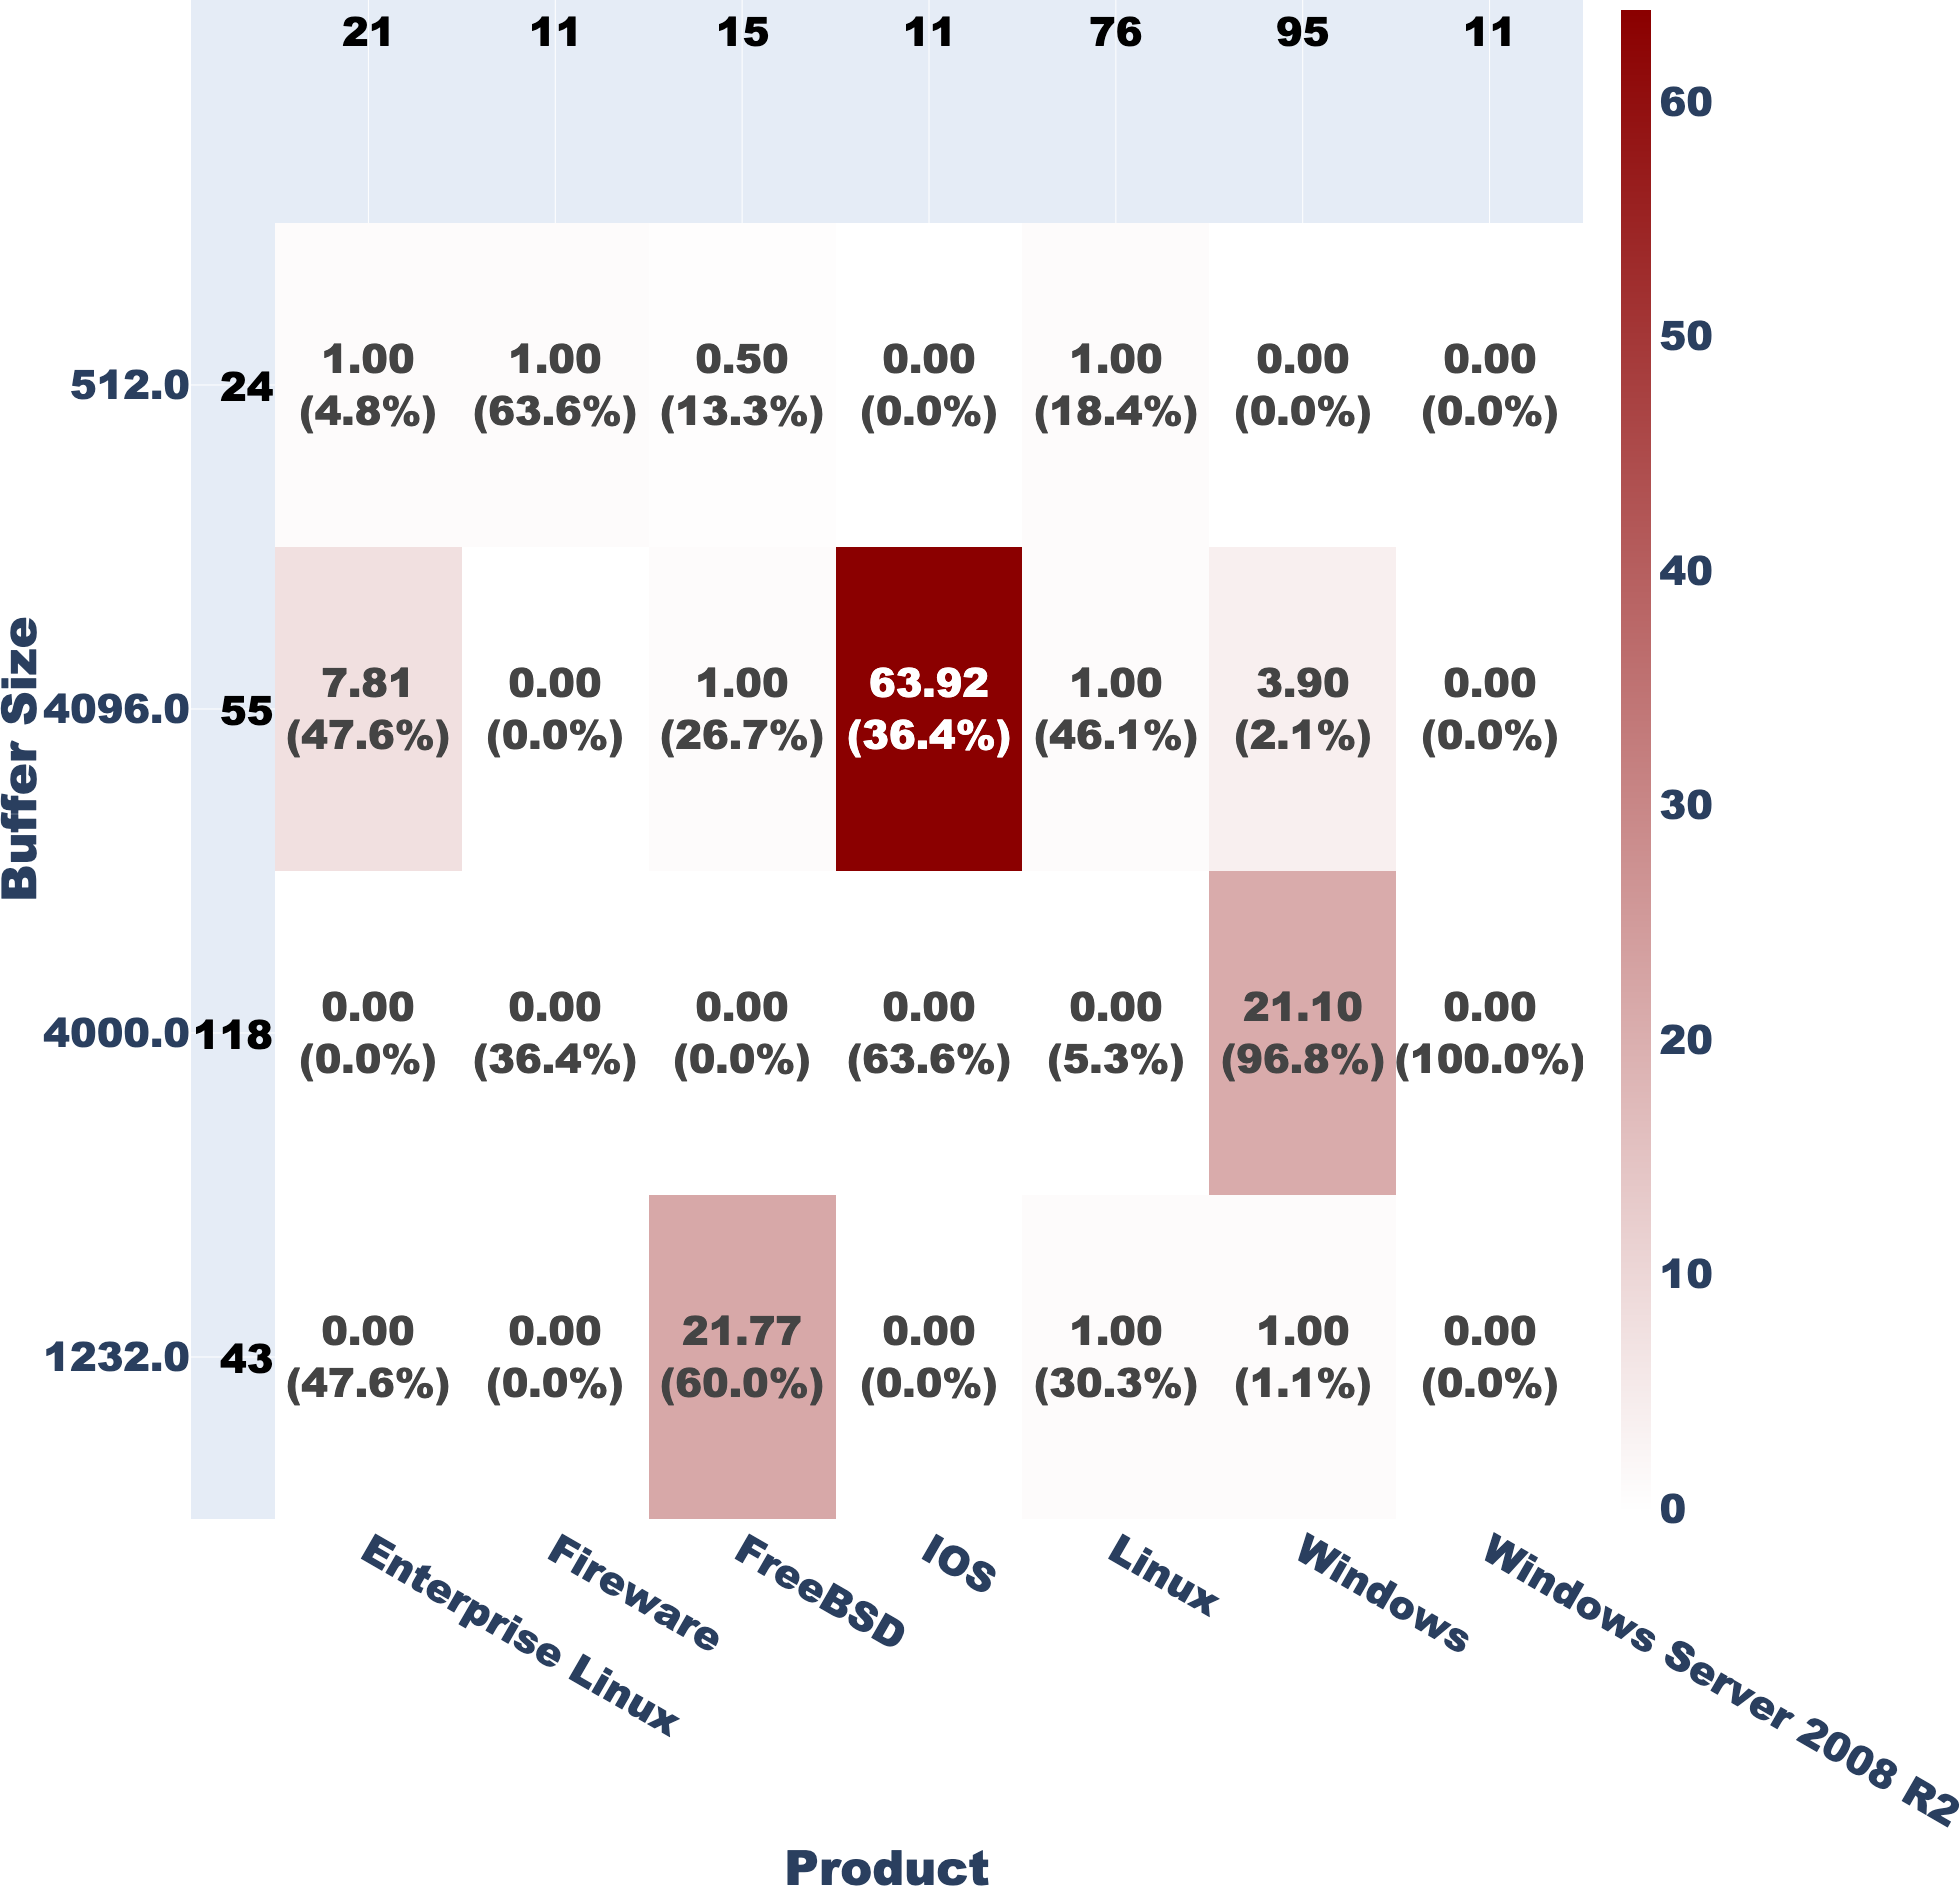
\includegraphics[width=\textwidth]{research paper/plots/filtered_Buffer Size_vs_Product_trim.png}
        \caption{Buffer Size against Product.}
        \label{fig:heatmap_buffer_product}
    \end{minipage}
\end{figure}


\section{Loopy attacks}
\label{appendix:loopy_attacks}
Below is a brief overview of the methodology created by~\cite{cispa-loopy} to find server pairs that are vulnerable to looping attacks. 

\looseness=-1 \textbf{Step 1.} In the first stage discovery packets are sent to all the servers go gather a complete set of responses. These could serve as the entry point to a traffic loop.  

\looseness=-1 \textbf{Step 2.} Since there could be many distinct responses (depending on the number of hosts), the second stage clusters the responses based on their semantics. Insignificant syntactic differences, such as the transaction ID (TXID), are ignored since they cannot influence a DNS response. In the end, several clusters will hold semantically equivalent responses. 

\looseness=-1 \textbf{Step 3.} With a similar reasoning as the second stage, in the third stage, random responses are sampled from each of the clusters. These will be the set of probes that will be sent again to each server. Sending all the initial responses to all the servers would have been both infeasible, due to the large number of initial responses, but also ineffective, since several packets from the same cluster are expected to have the same behaviour, and in turn, should themselves lead to the same response. The responses after this third stage also end up being clustered in the same way as the second stage.  

\looseness=-1 \textbf{Step 4.} With the information gathered in the third step, a loop graph can be formed. In this graph edges represent servers that reply to an input from one cluster with a response from the same or another cluster. Following this, a DFS is ran to find cycles with a length of at most 4.

\looseness=-1 \looseness=-1 \textbf{Step 5.} In the last stage, the loops that were identified previously are formally verified with a proxy. The proxy sits in between the two servers that are being tested and it forwards messages between the two. Once the proxy has forwarded enough messages, the two servers are validated as a loop pair. As this step required setting up a proxy, we have skipped it.

% \clearpage






% \section{Some further guidelines that go without saying (right?)}

% \begin{itemize}
% \item Read the manual for the Research Project. (See e.g.\ the instructions on the maximum length: less is more!)
% \end{itemize}

% \subsection{Reference use}
% \begin{itemize}
% \item use a system for generating the bibliographic information automatically from your database, e.g., use BibTex and/or Mendeley, EndNote, Papers, or \ldots
% \item all ideas, fragments, figures and data that have been quoted from other work have correct references
% \item literal quotations have quotation marks and page numbers
% \item paraphrases are not too close to the original
% \item the references and bibliography meet the requirements
% \item every reference in the text corresponds to an item in the bibliography and vice versa
% \end{itemize}

% \subsection{Structure}
% Paragraphs
% \begin{itemize}
% \item are well-constructed
% \item are not too long: each paragraph discusses one topic
% \item start with clear topic sentences
% \item are divided into a clear paragraph structure
% \item there is a clear line of argumentation from research question to conclusions
% \item scientific literature is reviewed critically
% \end{itemize}

% \subsection{Style}
% \begin{itemize}
% \item correct use of English: understandable, no spelling errors, acceptable grammar, no lexical mistakes 
% \item the style used is objective
% \item clarity: sentences are not too complicated (not too long), there is no ambiguity
% \item attractiveness: sentence length is varied, active voice and passive voice are mixed
% \end{itemize}

% \subsection{Tables and figures}
% \begin{itemize}
% \item all have a number and a caption
% \item all are referred to at least once in the text
% \item if copied, they contain a reference
% \item can be interpreted on their own (e.g. by means of a legend)
% \end{itemize}


\title{
    
\includegraphics[width=8cm, keepaspectratio]{tudelftlogo.png}\\
    \vspace*{2cm}
    \textbf{
        Estimating the Amplification Factor of Three Common Protocols in DRDoS Attacks\\
        % {\large A Measurement Study on the Weaponisation of Hosts from Greece}
        {\large A Quantitative Analysis on the Weaponization of Hosts Located in Greece}
        % {\large Assessing the Amplification Potential of Servers from Greece}
    }\\
    \vspace*{1cm}
}

\author{
     \textbf{
Rares-Andrei Toader$^1$}\\
    \hfill \break
    \textbf{Supervisors: Georgios Smaragdakis$^1$, Harm Griffioen$^1$ }\\
    \break
%    \affiliations
    {\large 
        \hfill \break
        $^1$EEMCS, Delft University of Technology, The Netherlands
    }\\
}

\date{}

\maketitle
\thispagestyle{empty}

\let\clearpagebackup\clearpage
\renewcommand{\clearpage}{ }

\onecolumn

\vspace*{1.5cm}
\begin{center}
    A Thesis Submitted to EEMCS Faculty Delft University of Technology,\\
    In Partial Fulfilment of the Requirements\\
    For the Bachelor of Computer Science and Engineering\\
    \today
\end{center}

\vspace*{2cm}

\noindent
{\small
Name of the student: Rares-Andrei Toader \\
Final project course: CSE3000 Research Project\\
Thesis committee: Georgios Smaragdakis, Harm Griffioen, Georgios Iosifidis	
\\
}
\vfill

\begin{center}
    An electronic version of this thesis is available at http://repository.tudelft.nl/.
\end{center}

\twocolumn
\let\clearpage\clearpagebackup  
\clearpage
\setcounter{page}{1}


\begin{abstract}
Distributed reflection denial-of-service (DRDoS) attacks are a type of cyberattack where a malicious actor sends requests to public and open servers on behalf of the victim by spoofing their IP address. The traffic generated by the corresponding responses is directed towards the victim (whose IP address appeared as the source address of the initial packets), potentially exhausting their bandwidth. These attacks have kept becoming more powerful over the years. 

This thesis presents a measurement study of three well-known protocols, where we assess the amplification potential of hosts located in Greece running these protocols. We find that DNS remains the most vulnerable protocol to amplification; the top 250 hosts can cumulatively amplify the traffic by 32,000$\times$. Furthermore, we discover that the ``ANY'' query type and the improperly configured DNS extension (EDNS0) are two significant causes of DNS amplification. Lastly, we also find hosts vulnerable to looping attacks, a novel threat in the context of DDoS attacks. 

% The aim of this template is to make it more clear what is expected from you. 
% \textbf{It is by no means required to follow this exact same structure.}
% The abstract should be short and give the overall idea:
% what is the background, the research questions, what are your contributions, and what are the main conclusions.
% It should be readable as a stand-alone text (preferably no references to the paper or to outside literature).
\end{abstract}

\section{Introduction}


% Malicious actors typically launch denial-of-service attacks to reduce the availability of Internet servers. 
\looseness=-1 A \textit{denial-of-service attack} (DoS) is a collection of cyber attacks that aim to disrupt the availability of a system~\cite{cloud_dos}. This attack and its variants have been widely researched~\cite{ddos_taxonomy} in the literature and have historically been one of the most popular strategies used by adversaries~\cite{crowdstrike_popular_attacks}. 

\looseness=-1 A \textit{distributed denial-of-service} (DDoS) attack has the same goal as a normal DoS attack~\cite{cloud_ddos}. However, it achieves this by having multiple adversarial entities exhausting the target's resources instead of a single attacking entity. DDoS is a more powerful attack than the normal DoS~\cite{cloud_ddos}. The attacking entities in a DDoS context could be compromised computers or infected IoT devices, which could be part of a larger, malicious entity called a \textit{botnet}~\cite{crowdstrike_botnet}. The target can be a web server or another network service. The flood of incoming packets or connection requests to the victim's system forces it to become slower, become unresponsive or even crash, denying regular service to legitimate users, thus violating the ``A'' (availability) from the CIA (Confidentiality, Integrity and Availability) triad~\cite{cia-triad}.

\looseness=-1 In a \textit{distributed reflection} DoS attack (DRDoS), a malicious actor uses public services to reflect traffic to a victim~\cite{amplification_hell}. The attacker sends requests on behalf of the victim, and in turn, the victim gets flooded with responses from the public services. Consequently, if enough requests are made and the size of the responses is large, the target's bandwidth is depleted. An amplification attack is essentially a DRDoS attack, where the attacker focuses on sending requesting packets to the public hosts, whose size would be smaller than the responding packets sent to the victim. In this sense, the response packets amplify the requesting packets, hence the attack's name. 

% IP Spoofing in UDP-based protocols makes it possible for an attacker to send packets on the victim's behalf. NEW

% The adversary must send packets on the victim's behalf to launch such an attack. This is possible due to IP spoofing in UDP-based protocols. OLD

\looseness=-1 Several reasons make amplification attacks possible. IP spoofing in UDP-based protocols makes it possible for an attacker to send packets on the victim's behalf. \textit{IP spoofing} means the attacker sets the source address in the IP header as the victim's IP address when sending a packet to a public server. Consequently, the victim receives the response packets from the servers. This happens because UDP-based protocols respond to queries without being required to establish a connection (which is the case for TCP-based protocols) and thus do not validate the IP address of the entity sending the request. IP spoofing is considered a bad practice, and measures for it have been described 24 years ago in an RFC (Request for Comments)~\cite{ferguson-2000}. This introduces the idea of network ingress filtering (commonly referred to as BCP38)~\cite{ferguson-2000}, which would be a general measure against denial-of-service attacks that utilise IP source address spoofing.  
However, empirical evidence shows that IP spoofing is an ongoing problem that has yet to be eliminated~\cite{spoofer_project}, remaining the most critical cause of amplification attacks~\cite{amplification_hell}.

\looseness=-1 Another essential cause for amplification attacks is an asymmetry between the size of a request to a public server and the size of the response. This asymmetry enables amplification and is a desirable feature for an attacker, as they only have to send a small packet to reflect a larger amount to the victim. This security issue is present in many protocols because these protocols have not been implemented with this aspect in mind. For example, the ``monlist'' command~\cite{cloud_monlist} allows users to query an NTP server, retrieving up to 600 hosts with which the NTP server has most recently communicated. This feature was mainly meant as a debugging tool but has also been weaponised by adversaries in successful DRDoS attacks~\cite{amplification_hell}.

\looseness=-1 The first DDoS attack happened in July 1999, more than 20 years ago~\cite{mit_first_ddos}. The biggest DDoS attack ever recorded took place in 2017~\cite{cloud_famoud_ddos}. It targeted Google services and peaked at 2.54 Tbps. DDoS attacks have kept getting more notoriety over the years, becoming well-established cyber attacks with a popularity that has kept rising. In a recent DDoS threat report for 2024 Q1, Cloudflare mentions that they have noticed a 50\% increase in DDoS attacks compared to the corresponding first quarter in 2023~\cite{cloud_q1report}. DDoS attacks are extremely popular in the cyber threat landscape for several reasons. Firstly, they are relatively easy to orchestrate, requiring little technical expertise, as they can even be bought online as a service, often under the umbrella name of ``stress-testing'', at a reasonable cost~\cite{buy_ddos}. Secondly, these attacks effectively overwhelm a victim's system, leading to downtime or service disruption. Moreover, the malicious actor can achieve this while also preserving their anonymity. 

\looseness=-1 Seeing the impact and complexity of DRDoS attacks, we realised there is no auditing tool to find servers in an autonomous system (AS)~\cite{autsys} that could be weaponised and, consequently, unintentionally participate in amplification attacks. The literature lacks a comprehensive list that enumerates all the negative aspects of all existing protocols or the configuration of a specific server that could contribute to launching an amplification attack.

\looseness=-1 As an extension, we also analyse looping attacks, a novel DoS attack at the application-layer level~\cite{cispa-loopy}. This particular attack leads to infinite amplification, as two vulnerable servers would send messages to each other indefinitely. This happens, for instance, when a host responds to a malformed request with an error message, and this response prompts another server to send the packet needed for the initial server to send the same error message. Thus, a traffic loop is formed between the two servers. This type of attack can be hazardous, as it could also be used to target network links. We follow the methodology in~\cite{cispa-loopy} to discover which servers are vulnerable and how many vulnerable host pairs could be formed. Note that our study focused on Greece, as this was the country assigned to us for our project. With this thesis, we make the following contributions:

\begin{itemize}[left=0pt, itemsep=0pt]
    \item We investigate which DNS, NTP, and Memcached servers located in Greece can be utilised in amplification attacks. 

    \item  We explore what amplification factor can typically be achieved with the Greek infrastructure explored and what conditions influence this factor. 

    \item We measure the number of vulnerable pairs of DNS and NTP servers located in Greece that could be formed in the context of looping attacks.
    
\end{itemize}



\looseness=-1 The thesis is structured as follows. In Section II, background information is given, such as definitions and important concepts. Section III mentions notable contributions related to our work. Section IV describes the data used in this work and how it was obtained. Section V presents the ways in which the experiments and measurements were performed. Section VI mentions the operational considerations enforced throughout this work in order to follow an ethical research procedure. Section VII highlights the results, and Section VIII showcases reflections on them. Lastly, Section VIII draws the conclusions. 







% \begin{itemize}
% \item Introduce the topic and explain why it is important (motivation!). %\emph{How should a scientific paper look like?}

% \item Relate to the most relevant existing work from the literature (use BibTeX), explain their contributions, and (critically) indicate what is still unanswered. 
% %\emph{The existing state of the art describes the setup of general scientific papers, e.g.\ see~\cite{hengl2002rules}, but this may be different for computer science papers.}

% \item Explain what the research questions for this work are. 
% This usually is a subset of the unanswered questions. %\emph{The aim of this work is therefore to provide a good template specifically for papers in the field of computer science.}

% \item Summarize the main contributions/conclusions of this research.
% NB: Make sure the title of the paper is a good match to the main research question / contribution / conclusion.

% \item Briefly indicate how the rest of the paper fits together to answer the research question(s).
% \end{itemize}

% For a longer research paper, a section with a more elaborate discussion of the literature may follow, but for short (conference) submissions, this is often included in the introduction.

% Make sure the introduction and conclusion are easily understandable by everyone with a computer science bachelor (e.g.\ your examiner may have a completely different expertise).

\section{Background}

\looseness=-1 This section provides details and definitions of relevant concepts in this thesis. We also give definitions and ways the considered protocols were used in amplification attacks in the past. 

\looseness=-1 An \textit{amplifier} is a public server running a UDP-based protocol. With this consideration, the server can receive spoofed requests and reflect the response to the victim. This paper considers servers running one of the following three services: the Domain Name System (DNS), the Network Time Protocol (NTP) and Memcached. The motivation behind restricting the research to these three services is that they have been notorious in the context of DRDoS, being potent amplification vectors~\cite{cloud_dns_ampl},~\cite{cloudflare_ntp_ampl},~\cite{cloud_memcached_ampl}. Nonetheless, for further work, other protocols are worth exploring, as shown in~\cite{amplification_hell}, such as the Simple Network Management Protocol (SNMP)~\cite{imperva_snmp}. 

\looseness=-1 To measure how powerful an amplifier is, we use the \textit{bandwidth amplification factor} (BAF) as this has been previously defined in the literature in the context of amplification attacks~\cite{amplification_hell}. BAF is defined as the quotient between the size of the UDP payload of the amplifier answer and the size of the UDP payload of the spoofed request, see Equation~\eqref{eq:baf}. 

\looseness=-1 For gathering information about hosts, such as IP addresses and services running on that server, we have used \textit{Censys}~\cite{censys15}. It is a search engine that enables security researchers to find and analyse devices and networks on the Internet quickly, without a heavy computational effort (via an academic license that we also received). Censys gathers data on hosts through periodic Internet scans, the scanning method relying on a variant of ZMap. This is a revolutionary scanner that can scan the entire IPv4 address range in around 45 minutes with enough bandwidth resources~\cite{zmap}. Censys scans and stores the ports of servers that are publicly accessible. The platform allows queries such as retrieving all hosts in Greece or hosts with a service running on a specific port. Queries used for this thesis along with some extra information are shown in Appendix~\ref{appendix:censys_queries}.

\looseness=-1 \textbf{Protocol Overview}. The \textit{Domain Name System} (DNS) is often described as the ``phonebook'' of the Internet~\cite{cloud_dns}. DNS forms the critical infrastructure that helps the browser find the assigned IP address of the server where the website is hosted, given the domain. DNS enables users to use simple, human-readable domain names that can be easily remembered and translated into IP addresses. This translation process is the so-called \textit{address resolution}. DNS usually runs on port 53 and can handle many other types of requests, responding with corresponding resource records (RRs). If someone sends an ``ANY'' request, the DNS server answers with all the resource records related to the domain queried.  For this reason, DNS represents an attractive amplification vector for malicious adversaries. It does not surprise that according to Cloudflare, in 2021, 44\% of organisations mentioned that attacks based on DNS were one of their most challenging security problems~\cite{cloud_dns_threat_landscape}.


\begin{figure}[t]
  % \vspace*{-\dimexpr\topskip+\ht\strutbox\relax} 
    \small
    \begin{equation}
    BAF = \frac{len(UDP\ payload)\ amplifier\ to\ victim}{len(UDP\ payload)\ attacker\ to\ amplifier}
    \label{eq:baf}
    \end{equation}
\end{figure}

\vspace{-0.68pt}
% NTP
\looseness=-1 The \textit{Network Time Protocol} (NTP) is a protocol used to synchronise the clocks between computers over a network~\cite{wiki_ntp}. Essentially, it ensures that all the computers connected to a network agree on the time, up to an accuracy of milliseconds. This is crucial for tasks that require precise timing, such as logging events or scheduling tasks. Implementations of this protocol commonly use the port number 123 and exchange timestamps over UDP~\cite{wiki_ntp}. NTP has been weaponised previously via the ``monlist'' command, which returns a list of up to 600 hosts that most recently communicated with an NTP server~\cite{cloudflare_ntp_ampl}.  This is prone to creating significant responses compared to a small query, leading to an enormous amplification factor. Mitigations have been proposed; K{\"u}hrer et al. explored this vulnerability and managed to carry out a campaign that, in the end, reduced the susceptible NTP servers by a staggering 92\%~\cite{exit_hell}. We aim to investigate whether the NTP ``monlist`` command is still a threat to the Greek network infrastructure.

% Memcached

\looseness=-1 \textit{Memcached} is a distributed memory caching system primarily used to increase the performance of dynamic web applications by removing some load from the database~\cite{memcached_github}. It works by storing data from the result of database calls, API calls, or page rendering in memory (essentially being cached). The data is stored in the random-access memory (RAM) of the servers running the Memcached daemon and is structured as a sizeable hash table distributed across machines~\cite{wiki_memcached}. This means that when the same data is needed again, it can be retrieved faster from this memory cache rather than being recomputed or fetched from a slower disk-based database.  Memcached services often run on port 11211 and sometimes respond to UDP requests~\cite{wiki_memcached}. GitHub sustained a heavy DRDoS attack in 2018 based on the Memcached ``get'' query. This attack was described by Akamai in 2018, and it presented how such a query could lead to a potential amplification factor of $50,000$~\cite{akamai2018attackspotlight}. 

% This request sends the value associated with a key (which can have an extreme size, up to 1 MB)~\cite{wiki_memcached}. After the GitHub attack, Memcached-based attacks have dropped in popularity due to vendors patching their software. We investigate if this devastating attack is still possible in the wild. 




% \textbf{Tool Overview}. \textit{Scapy} is a versatile packet manipulation library~\cite{scapy} used in this thesis to construct, send and capture packets to measure the amplification factor. It can create and parse packets of numerous protocols, send them and receive and match response packets to requests. Scapy can parse the packets, providing details such as packet structures and payload sizes. It can be used in an interactive shell as a REPL or in Python as a library. For this thesis, we used the latter.


% The \textit{Domain Information Groper} (dig) is a useful command-line tool that enables users to query DNS name servers in a simple manner. It fetches DNS information (DNS records) about domain names, mail exchanges, IP addresses and name servers. Being easy to use and flexible, it is the standard tool system administrators use to diagnose DNS problems and examine DNS configurations. We have used it in our research to find authoritative name servers for a set of domains easily and to map domain names to IP addresses. 
 
% As data from Censys came in JSON format, we have used \textit{jq} to retrieve specific fields and records from the JSON file~\cite{jq}. It is a lightweight command-line tool that allows users to process JSON, extract and modify elements, and produce JSON or even CSV outputs, making it very useful for working with JSON-formatted data.



\section{Related Work}

\looseness=-1 This section describes existing research in the field of amplification attacks. Rossow~\cite{amplification_hell} did a comprehensive study of how suitable 14 popular UDP-based protocols are for amplification attacks. The results of this study were quite worrying, as the author found millions of amplifiers that could be used in a distributed attack for six protocols. We similarly assess the amplification potential of DNS and NTP. The paper also explores methods to detect DRDoS attacks in the wild using traffic analysis. Lastly, Rossow also presents  DRDoS mitigation techniques and ways to strengthen network protocols against this type of attack. 


\looseness=-1 Griffioen et al.~\cite{griffioen_scan_2021} explored the steps an attacker takes when orchestrating an amplification attack by observing a set of honeypots deployed in the wild. We followed a methodology akin to the one the authors presented. Their work also discovered that attackers have a shared memory of previously used servers in amplification attacks. Still, attackers differ in how they orchestrate such an attack, the landscape being filled by both novice actors and very sophisticated adversaries. 


\looseness=-1 Van der Toorn et al.~\cite{van_der_toorn_anyway_2021} researched the amplification potential of domain names in the context of ``ANY'' queries, and what the reduction in response size would be if ``ANY'' queries would be dropped, according to the suggestions of RFC 8482~\cite{rfc-8482}. They also proposed and validated a technique to approximate the size of responses to ``ANY'' requests based on a large active DNS measurement dataset. We crafted our DNS query (the one we measure the amplification factor with) following what the authors also proposed. 

\looseness=-1 Kührer et al.~\cite{exit_hell} studied the diversity of amplification sources, finding that they spread across various operating systems. A crucial impact of their paper was that they carried out a large-scale campaign to alert NTP administrators about the amplification potential of answering the ``monlist'' request. As a result, this campaign led to more than a 92\%  decrease in vulnerable NTP servers. Their work also highlights vulnerabilities in the TCP handshake that attackers could use as amplification vectors, which we will not explore as it is outside the scope of our research. They conclude that the root cause for amplification attacks is the fact that there are networks that allow IP address spoofing. 

\looseness=-1 Pan et al.~\cite{cispa-loopy} researched a novel and hazardous type of denial-of-service attack at the application layer. The \textit{looping attack} allows a malicious actor to send one IP-spoofed packet to a server that, in turn, triggers an infinite loop of back-and-forth messages between the server to whom the packet was sent and the server whose IP was spoofed in the initial request. This essentially enables infinite amplification. They propose a systematic methodology to search for vulnerable server pairs. They further use this methodology to investigate loops that can be formed with servers running various UDP protocols. The results were quite jarring, as an attacker could potentially abuse billions of server pairs for looping attacks. For this reason, we chose to study if hosts located in Greece are also susceptible to this type of attack. 



% \looseness=-1 Wagner et al.~\cite{wagner_united_2021} investigate the potential of enhanced mitigation through collaborative efforts at the Internet Exchange Points (IXPs) level. The central assumption they prove is that sharing data between IXPs leads to a higher percentage of detected DDoS attacks. Over 120k attacks are analysed, and a significant finding is that more than 80\% of these attacks remain undetected by local mechanisms due to imperfect local thresholds and the complex nature of attacks using multiple protocols. Their collaborative approach enhanced local attack detection, reducing up to 90\% more attack traffic. This highlights the role that core internet infrastructures (such as IXPs) play in detecting and mitigating DDoS attacks. We do not analyse this technique further. However, we underline its effectiveness and its positive effect on reducing the impact of DRDoS attacks.



\section{Datasets}
\looseness=-1 This section presents the sources of the data used for our research. Four primary data sources were inspected. The first data source is Censys~\cite{censys15} with their Internet database, and the second is IANA~\cite{iana} to find all top-level domains. The third is NTP Pool~\cite{ntp_pool} and the fourth source is an archived list of the most popular domain names from the Technical University of Munich (TUM)~\cite{tum_domains}.

\looseness=-1 \textbf{Host information}. Censys offers a large variety of publicly available information related to the public Internet. The platform allows for queries similar to those in a search engine. We used this functionality to query for hosts located in Greece (via passive scanning), which are running DNS, NTP, and Memcached on ports 53, 123 and 11211, respectively. The three queries (one per protocol) can be seen in Appendix~\ref{appendix:censys_queries}. The output from the queries came as raw JSON files containing a list of IP addresses alongside relevant metadata such as location or AS. After processing the data, we were left with 7,532 (DNS), 25,962 (NTP) and 13 (Memcached) servers. 

\looseness=-1 The data was collected on May 10, 2024. Still, since we employed passive scanning (we just queried whatever data was stored; we did not actively probe servers at this stage), we are unaware of the actual date of origin when Censys collected the data. 

\looseness=-1 \textbf{Top-level domains}. The \textit{Internet Assigned Numbers Authority} (\textit{IANA}) is an organisation that is responsible for allocating IP addresses, AS numbers and other tasks~\cite{iana}. We used it to gather a list of all available top-level domains (TLDs). This data was collected on May 2, 2024. 

\looseness=-1 The list of all TLDs is later ranked based on which domain is associated with the largest response size. That domain is later used in DNS ``ANY'' queries. The rationale behind this decision is that ranking all possible domains requires much more computational effort and is outside the scope of this work. However, this is an interesting topic, which has been researched by Van der Toorn et al.~\cite{van_der_toorn_anyway_2021}. In this work, they rank hundreds of millions of domain names based on the amplification factor they can achieve. Another insightful finding they discovered is that the domains used in DNS-based DDoS attacks are among the largest ones that could be used. Furthermore, even larger domains that had yet to be exploited were found.

\looseness=-1 \textbf{NTP Pool servers}. The NTP Pool project represents a sizeable virtual cluster of NTP servers distributed worldwide~\cite{ntp_pool}. This pool is critical in synchronising clocks for millions of machines worldwide. We found 12 NTP servers located in Greece that were part of this group as of May 3, 2024. We considered that they were worth testing for amplification since many clients use the pool. Although all 12 NTP servers were open, none of them were found to be vulnerable to amplification.

\looseness=-1 \textbf{Most popular domain names}. From the archive by TUM, we obtained the top 10 million domain names according to Open PageRank as of April 16, 2023~\cite{tum_domains}. This dataset was used to find popular Greek domain names. We kept the most popular 1,023 Greek domains. Consequently, these helped us find authoritative nameservers located in Greece.
    
\looseness=-1 Using the first three datasets, we were able to make precise measurements of the amplification potential of DNS, NTP, and Memcached hosts located in Greece. The last dataset enabled us to see whether authoritative nameservers can serve as better amplifiers than non-authoritative ones in the context of DNS-based amplification attacks.


% openpagerank-top-10m-2023-04-16_0900_UTC.csv
% Min 300 words

% Censys => host IP addresses corresponding to servers running NTP, DNS and Memcached




% \section{Your contribution (replace this section title by something more informative)}
% In computer science typically the third section contains an exposition of the main ideas, for example the development of a theory, the analysis of the problem (some proofs), a new algorithm, and potentially some theoretical analysis of the properties of the algorithm.

% Do not forget to give this section another name, for example after the method or idea you are presenting.

% Some more detailed suggestions for typical types of contributions in computer science are described in the following subsections.


% \subsection*{Experimental work}
% In this case, this section will mostly contain a description of the methods/algorithms you will be comparing. Although not all methods need to be described in detail (providing appropriate references are available), make sure that you reveal sufficient details to a reader not familiar with these methods to: a) obtain a high-level understanding of the method and differences between them, and b) understand your explanation of the results/conclusions.

% \subsection*{Improvement of an idea}
% In this case, you would need to explain in detail how the improvement works. If it is based on some observation that can be proven, this is a good place to provide that proof (e.g., of the correctness of your approach). 

% \subsection*{Literature survey}
% If your contribution is a literature survey, then the organization of these ``middle'' sections very much depends on the way you want to present/organize the literature you are discussing.
% First try to cluster papers that are similar in some aspect. Then think of how these clusters are related, from that you can think of a good order to discuss these clusters; this is sometimes called a bottom-up approach to writing a paper.

% In addition, you may try to think about the organization of the literature from a top-down perspective: try to ``take a step back'' and think about the field and what important questions/variants are and build a hierarchical categorization of the field.

% Make clear what your contribution is here: a new organization of the literature, identification of open problems/challenges, new parallels/generalizations, a table with pros/cons of different methods, etc.\ 



\section{Methodology}

\looseness=-1 In this section, we present the methodology for measuring the amplification potential of servers located in Greece, alongside a brief description of how we counted the number of server pairs vulnerable to looping attacks. An overview of our methodology can be seen in Fig.~\ref{fig:diagram}.

\captionsetup{font=small}
\begin{figure}[t]
  \centering
  \includegraphics[width=0.4838\textwidth]{research paper/plots/diagram_trim.png}
  \caption{Methodology diagram. The top left side corresponds to collecting authoritative nameservers. The top right part shows how to find the server pairs vulnerable to looping attacks using the methodology from the correspondent paper.}
  \label{fig:diagram}
\end{figure}


\looseness=-1 \textbf{Measuring the amplification potential}. To accurately measure the BAF of hosts located in Greece running DNS, NTP or Memcached, we have followed a similar methodology to the one presented by Griffioen et al.~\cite{griffioen_scan_2021}. We mimicked an adversary's workflow without actually launching a DDoS attack.


\looseness=-1 \textbf{Filtering closed hosts}. Firstly, we have gathered and processed host information (the so-called ``Reconnaissance'' phase). An attacker would first be interested in seeing whether these servers are ``online'', i.e. accepting and responding to requests, as this is the prime precondition to be weaponised. This step allowed us to avoid doing unnecessary work on offline hosts. This step reduces the computational load on our machine and any strain we might put on the network. Thus, a filtering step would be essential if such a measurement study was conducted worldwide. More details for each filtering packet presented below can be seen in Appendix~\ref{appendix:filter_queries}.

\looseness=-1 We hand-crafted packets for each protocol, which we then sent to hosts, and filtered out servers that did not respond with a packet we expected, for instance, returning an ICMP error packet or hosts that did not respond within a timeout period we set. The packets we crafted were aimed to be basic, common packets that an open server would be expected to answer without any issue. This measure is by no means foolproof and could be improved by sending more than one probe per protocol.
    
\looseness=-1 \textbf{DNS}. We send a simple request (query type = ``A'') to resolve the IP address of ``google.com'', with the rationale that this domain is widespread and almost any open recursive DNS resolver would be able to answer it (by retrieving the appropriate record from the corresponding authoritative nameserver). Recursive resolvers, as opposed to authoritative nameservers, do not hold the answer RRs, but they make the necessary requests on behalf of the client (if the result was not cached). In this part, we were aware that we might be biased towards filtering out authoritative NSs since they are less likely to hold the ``A'' RR requested (a limited number of servers have this record). They might still retrieve them if they forward the request to another resolver in case of an error. However, this is unexpected behaviour and a bad practice~\cite{auth_no_rec}; even an RFC from 2008 mentions that, in general, authoritative NSs should not provide recursion~\cite{rfc-5358}. 

\looseness=-1 The bias to discard authoritative NSs is hard to measure since DNS servers do not respond, admitting they are authoritative. To mitigate this, we performed a procedure to complement our DNS host set, which will be explained later, by collecting authoritative NSs. We reject responses with ``rcode'' set to 2 or 5, which stands for server failure and refused, respectively. We also set a timeout of 400 milliseconds. The filtering step left us with 2,397 servers.
        
\looseness=-1 \textbf{NTP}. We create a simple Mode 3 packet, i.e. a ``client mode'' packet. This is one of the several operational modes of NTP, and it allows a ``client'' to query a server for the current time. In a sense, it represents the core functionality of NTP. To validate this approach, we looked at how the ``sntp'' command-line utility tool~\cite{sntp_overview} crafts packets (by capturing the packets sent and inspecting them via Wireshark~\cite{wireshark}), and we noticed they send the exact packet we crafted with Scapy, a robust packet manipulation tool with Python support~\cite{scapy}. We rejected any non-NTP response and set a timeout period of 200 milliseconds. This step left us with 25,130 servers. We then proceeded with another filtering stage, as we are only interested in Mode 7 queries (they lead to the highest amplification); we also sent the notorious ``monlist'' command by setting the request code to $42$~\cite{cloud_monlist}. A timeout period of 1 second was set, and any non-NTP response packets were not considered. The dataset was further reduced to 633 servers. 

\looseness=-1 \textbf{Memcached}. A ``stats slabs'' packet is created to query the Memcached server for detailed statistics about the memory allocation. Memcached uses a slab allocation technique to manage memory efficiently for storing items of various sizes~\cite{slab_allocation}. Slabs are essentially blocks of memory divided into chunks. Each chunk can hold a cached item. When this packet is sent, Memcached is supposed to answer with information about each slab class, including the number of chunks allocated or used. After this was carried out, 0 out of 13 were left standing. This shows that none of the Memcached servers located in Greece responded to UDP. Turning off the UDP port for Memcached had been a widely deployed security measure following a sequence of devastating attacks exploiting this protocol~\cite{amplification_hell}.
    

\looseness=-1 \textbf{Augumenting DNS dataset}. To ensure our DNS dataset also has a representative sample of authoritative servers, we decided to retrieve top Greek domains from the list provided by TUM (see Section \RNum{4}). We parsed enough of the list to obtain a good amount of domains. We obtained 1,023 Greek domains. We queried our local resolver for ``NS'' records on the Greek domains to find authoritative nameservers. We then performed a DNS query for the nameserver domains to resolve their IP addresses. As a final check, we made sure that the IPs were in Greece's IP range by using ipinfo~\cite{ipinfo}, an insightful geolocation tool for IPs. Thus, we collected 926 authoritative nameservers and the domains each one was authoritative for.  

\looseness=-1 \textbf{Collect amplification factors}. Secondly, we wish to rank the filtered hosts based on the BAF (see Equation~\eqref{eq:baf}). For this purpose, we again hand-crafted special packets for each protocol. Having the attacker's reasoning in mind, we wanted to create the packets that would lead to the highest amplification factor. Appendix~\ref{appendix:measurement_queries} shows other details (e.g. code) related to these packets.

\looseness=-1 \textbf{DNS}. An adversary aims to make the query size smaller, i.e. query a smaller domain, while getting substantial responses. This could happen if the attacker creates a short domain with a large ``TXT'' record, for instance. However, we assumed that an attacker would like to leave as few traces as possible and use existing domains. Since there are millions of domains, we restricted ourselves to rank only the top-level domains (the list retrieved from IANA mentioned in Section \RNum{4}) according to their BAF. We used the well-established ``ANY'' query for the following measurements, as attackers typically used it in DNS-based amplification attacks too~\cite{van_der_toorn_anyway_2021} since nameservers (if they support this query type) are expected to return all RRs of the domain in the query. 
    
\looseness=-1 The TLDs are among the shortest domains one could use in a query. Surprisingly, ``.sl'' (the country-code top-level domain for Sierra Leone) returned the highest BAF of 177.83. This was an extreme value and is also a theoretical one as the response size had 5,513 bytes (larger than the maximum UDP size of 4,096) and was sent over TCP. This motivated us enough that the domain contained many records and was a worthy candidate for the query. Note that this measurement was done on all TLDs using the Google Public DNS recursive resolver (8.8.8.8) to ensure reproducibility~\cite{google_dns}. We then proceeded to query the DNS hosts with the ``ANY'' query on the ``.sl'' domain, with an EDNS0 record setting the buffer size to 4,096 and the ``DO'' bit set to 1 (to request a DNSKEY signed answer), following the methodology of~\cite{van_der_toorn_anyway_2021}, as we were interested in getting the maximum response. We got a BAF as high as 132.19, which is still very attractive for an attacker. This query was expected to yield small amplification factors for the authoritative nameservers, so we performed the same query on a different domain instead. We made one request per domain for which the nameservers were authoritative and kept the maximum BAF attained.
    
\looseness=-1 \textbf{NTP}. Alongside the notorious ``monlist'' (mon\_getlist\_1), we also sent three other Mode 7 (private) packets, namely peer\_list, peer\_list\_sum and get\_restricted, as they were also known to lead to good amplification factors~\cite{rapid7_private}. The ``peer\_list'' request will return all hosts with whom a server is peering, ``peer\_list\_sum'' returns the same information as the previous request but also includes some metadata about the peers. Lastly, a ``get\_restrict'' response will contain hosts to whom firewall rules are applied (e.g., allowlisted IPs or blocklisted). If a server responds to the last query, this also leads to an information disclosure vulnerability attack. 
    
\looseness=-1 \textbf{Memcached}. Following the 1.3Tbps DDoS Attack on GitHub~\cite{wired_ddos}, Akamai disclosed the type of queries attackers sent to public Memcached servers~\cite{akamai2018attackspotlight}. Even though none of our servers responded to UDP requests, we decided to still work on the methodology to send a packet that is expected to get a significant response from Memcached servers. We also validated the methods on an open Memcached server from one of our peers from France. It is important to note that Memcached operates in its essence in a very similar fashion to a key-value store. Users can query using a ``get $<$key$>$'' command to retrieve the value assigned to the key. Typically, the maximum size of a value is 1 megabyte (MB). An attacker can use this command on an existing key (that is short) associated with a considerable value. However, maximum effectiveness is achieved when the attacker sets the smallest key possible (with the size of 1 character) to the largest value possible (1 MB of data). After this, the ``get'' command can be sent alongside the key inserted previously. An attacker can even chain the keys, sending ``get $<key>$ $<key>...$'', which would lead to a tremendous response. This type of packet was observed in~\cite{akamai2018attackspotlight}. The strategy will lead to an amplification factor in tens of thousands, which is unprecedented compared to the other protocols studied. We decided to work with whatever was stored on the server and compute the BAF for a ``get'' request with a single key, namely the one with the largest associated value (so without implanting a key and value pair). More details and our implementation of this approach are presented in Appendix~\ref{appendix:measurement_queries}.


\looseness=-1 \textbf{Gather factors}. To investigate which servers achieve a large or small BAF adjacent to our measurements, we also collect metadata that will later be analysed in conjunction with the amplification factor. This has been done to paint a better picture of what leads to a higher amplification factor. The code that supports the collection of factors can be seen in Appendix~\ref{appendix:collect_metadata}.

\looseness=-1 For DNS, we collected the software run by hosts by fingerprinting using ``fpdns''~\cite{fpdns_kirei}. From the initial Censys data, we collected various information about the AS, such as the AS description and the AS number, as well as the vendor (i.e. Microsoft) and the product (operating system, i.e. Linux). By using the ``dig'' command~\cite{dig}, a flexible DNS lookup utility tool, we also retrieved what EDNS0 buffer size a DNS server was advertising (if any). For NTP, we fetched the system variable (i.e. operating system) of each host by using the ``ntpq'' utility tool~\cite{ntpq}.
    
\looseness=-1 \textbf{Vulnerability to looping attacks}. Besides the BAF measurement, we analyse the same protocol pairs for DNS and NTP, which are vulnerable to looping pairs. To do this, we followed the methodology and ran the same experiments as Pan et al.~\cite{cispa-loopy}. We forked the repository in order to run the code (after making some small changes for the scale of our experiment) on our datasets~\cite{loopy_code}. The procedure they set up is composed of 5 steps, which are detailed in Appendix~\ref{appendix:loopy_attacks}. Due to the difference in size of the datasets (we had around 100 times fewer hosts), we had to adapt the code and change some of the authors' decisions. After the second step, they find 90 clusters with at least $10,000$ responses, and they only sample packets from these clusters in step 3. In our experiment, we considered all the clusters with at least $1$ response. Furthermore, in step 4, the authors only consider edges with at least $100$ participants, whereas we kept all edges with at least $2$ participants (not $1$, to avoid self-loops). We have also skipped running the last stage, which would have involved setting up a proxy. If this had been done incorrectly, we would have risked starting an actual loop between two servers.

% \begin{enumerate}[itemsep=0pt]
% \looseness=-1 \textbf{Step 1.} In the first stage discovery packets are sent to all the servers go gather a complete set of responses. These could serve as the entry point to a traffic loop.  

% \looseness=-1 \textbf{Step 2.} Since there could be many distinct responses (depending on the number of hosts), the second stage clusters the responses based on their semantics. Insignificant syntactic differences, such as the transaction ID (TXID), are ignored since they cannot influence a DNS response. In the end, several clusters will hold semantically equivalent responses. 

% \looseness=-1 \textbf{Step 3.} With a similar reasoning as the second stage, in the third stage, random responses are sampled from each of the clusters. These will be the set of probes that will be sent again to each server. Sending all the initial responses to all the servers would have been both infeasible, due to the large number of initial responses, but also ineffective, since several packets from the same cluster are expected to have the same behaviour, and in turn, should themselves lead to the same response. The responses after this third stage also end up being clustered in the same way as the second stage.  

% \looseness=-1 \textbf{Step 4.} With the information gathered in the third step, a loop graph can be formed. In this graph edges represent servers that reply to an input from one cluster with a response from the same or another cluster. Following this, a DFS is ran to find cycles with a length of at most 4.

% \looseness=-1 \looseness=-1 \textbf{Step 5.} In the last stage, the loops that were identified previously are formally verified with a proxy. The proxy sits in between the two servers that are being tested and it forwards messages between the two. Once the proxy has forwarded enough messages, the two servers are validated as a loop pair. As this step required setting up a proxy, we have skipped it.
% \end{enumerate}

% \captionsetup{font=scriptsize}
% \begin{table}[t]
%     \raggedright % Aligns the table to the left
%     \caption{BAF per protocol. ``All'' represents the mean BAF across all open amplifiers, 50\% and 10\% only consider the most vulnerable 50\% or 10\% of all open amplifiers. In the third column, in the NTP row, the first number shows the number of servers that responded to a Mode 3 request, and the second the hosts that responded to ``monlist''.}
%     \scriptsize % Reduce font size (tiny is even smaller) /scriptsize
%     \renewcommand{\arraystretch}{0.8} % Adjust row height
%     \setlength{\tabcolsep}{1.3pt} % Adjust column spacing
%     \begin{tabular}{lcccccc}
%         \toprule
%         \multirow{2}{*}{Protocol} & \multirow{2}{*}{\# of hosts} & \multirow{2}{*}{\# of open hosts} & \multicolumn{3}{c}{BAF} & \multirow{2}{*}{Strategy} \\
%         \cmidrule(r){4-6}
%          &  &  & All & 50\% & 10\% &  \\
%         \midrule
%         DNS & 7532 & 2398 & 16.5 & 33.1 & 128.5 & ``ANY'' on ``.sl'' \\
%         DNS\(_{auth}\) & 926 & 926 & 11.8 & 18.4 & 26.0 & Max. ``ANY'' on own domains\\
%         NTP & 25962 & 25129 / 632 & 2.8 & 4.7 & 19.1 & Max. of private queries\\
%         Memcached & 13 & 0 & 0 & 0 & 0 & ``Get'' request \\
%         \bottomrule
%     \end{tabular}
%     \label{tab:hosts_baf}
% \end{table}

% \looseness=-1 Due to the difference in size of the datasets (we had around 100 times fewer hosts), we had to adapt the code and change some of the authors' decisions. After the second step, they find 90 clusters with at least $10,000$ responses, and they only sample packets from these clusters in step 3. In our experiment, we considered all the clusters with at least $1$ response. Furthermore, in step 4, the authors only consider edges with at least $100$ participants, whereas we kept all edges with at least $2$ participants (not $1$, to avoid self-loops). We have also skipped running the last stage, which would have involved setting up a proxy. If this had been done incorrectly, we would have risked starting an actual loop between two servers.

% As we want to promote open research, the code for the experiments and the datasets, including results, will be publicly available on the author's GitHub account.



% !! overview with results table!!  























 
% \section{Experimental Setup and Results}
% As discussed earlier, in many sciences the methodology is explained in section 2 and this section only discusses the results. 
% However, in computer science, most often the details of the evaluation setup are described here first (simulation environment, etc.).
% Very important is that any skilled reader would be able to reproduce this setup and then obtain the same results.

% Then, results are reported in an accessible manner through figures (preferably with captions that allow them to be understood without going through the whole text), observations are made that clearly follow from the presented results.
% Conclusions are drawn that follow logically from the previous material.
% Sometimes the conclusions are in fact hypotheses, which in turn may give rise to new experiments to be validated.

% You may want to give this section another name.

\section{Responsible Research}



\captionsetup{font=scriptsize}
\begin{table}[t]
    \raggedright % Aligns the table to the left
    \caption{BAF per protocol. ``All'' represents the mean BAF across all open amplifiers, 50\% and 10\% only consider the most vulnerable 50\% or 10\% of all open amplifiers. In the third column, in the NTP row, the first number shows the number of servers that responded to a Mode 3 request, and the second the hosts that responded to ``monlist''.}
    \scriptsize % Reduce font size (tiny is even smaller) /scriptsize
    \renewcommand{\arraystretch}{0.8} % Adjust row height
    \setlength{\tabcolsep}{1.3pt} % Adjust column spacing
    \begin{tabular}{lcccccc}
        \toprule
        \multirow{2}{*}{Protocol} & \multirow{2}{*}{\# of hosts} & \multirow{2}{*}{\# of open hosts} & \multicolumn{3}{c}{BAF} & \multirow{2}{*}{Strategy} \\
        \cmidrule(r){4-6}
         &  &  & All & 50\% & 10\% &  \\
        \midrule
        DNS & 7532 & 2398 & 16.5 & 33.1 & 128.5 & ``ANY'' on ``.sl'' \\
        DNS\(_{auth}\) & 926 & 926 & 11.8 & 18.4 & 26.0 & Max. ``ANY'' on own domains\\
        NTP & 25962 & 25129 / 632 & 2.8 & 4.7 & 19.1 & Max. of private queries\\
        Memcached & 13 & 0 & 0 & 0 & 0 & ``Get'' request \\
        \bottomrule
    \end{tabular}
    \label{tab:hosts_baf}
\end{table}

\looseness=-1 This section will present the considerations we made when conducting our experiments to follow an ethical research approach. 

\looseness=-1 \textbf{Ethical Considerations}. When gathering initial information about hosts, we employed passive scanning to be as non-intrusive as possible. In contrast, if done without proper authorisation, active scanning could have been seen as malicious by the other parties. Furthermore, in the filtering and measurement stage of our methodology, described in Section \RNum{5}, we send packets to a host once, and we set a cool-down period of 100 milliseconds between requests to prevent flooding the target with requests, as well as not exhausting the bandwidth of any network links, respectively. 

\looseness=-1 We will also make sure not to publish the IP addresses of hosts that are amplifiers to avoid the possibility of an attacker using this information and launching a DDoS attack. We wish to refrain from facilitating anyone with the resources to carry out such an attack. 
 

\looseness=-1 \textbf{Reproducibility}. Due to the dynamic character of the world's networks, it is impossible to guarantee the complete reproducibility of our experiments. For instance, due to IP address churn, the hosts we gathered might have different IPs if collected at different times in the future~\cite{griffioen_quantifying_2020}. Similarly, the vantage point from which the experiments are conducted might influence the results~\cite{wagner_united_2021}. Nonetheless, we have created a Dockerfile that specifies everything one needs to run our experiments in the same setting (i.e., the same dependencies and versions). The scripts are also open-source and hosted on the author's GitHub~\cite{rares_code}. 


% \captionsetup{font=scriptsize}
% \begin{table}[t]
%     \raggedright % Aligns the table to the left
%     \caption{BAF per protocol. ``All'' represents the mean BAF across all open amplifiers, 50\% and 10\% only consider the most vulnerable 50\% or 10\% of all open amplifiers. In the third column, in the NTP row, the first number shows the number of servers that responded to a Mode 3 request, and the second the hosts that responded to ``monlist''.}
%     \scriptsize % Reduce font size (tiny is even smaller) /scriptsize
%     \renewcommand{\arraystretch}{0.8} % Adjust row height
%     \setlength{\tabcolsep}{1.3pt} % Adjust column spacing
%     \begin{tabular}{lcccccc}
%         \toprule
%         \multirow{2}{*}{Protocol} & \multirow{2}{*}{\# of hosts} & \multirow{2}{*}{\# of open hosts} & \multicolumn{3}{c}{BAF} & \multirow{2}{*}{Strategy} \\
%         \cmidrule(r){4-6}
%          &  &  & All & 50\% & 10\% &  \\
%         \midrule
%         DNS & 7532 & 2398 & 16.5 & 33.1 & 128.5 & ``ANY'' on ``.sl'' \\
%         DNS\(_{auth}\) & 926 & 926 & 11.8 & 18.4 & 26.0 & Max. ``ANY'' on own domains\\
%         NTP & 25962 & 25129 / 632 & 2.8 & 4.7 & 19.1 & Max. of private queries\\
%         Memcached & 13 & 0 & 0 & 0 & 0 & ``Get'' request \\
%         \bottomrule
%     \end{tabular}
%     \label{tab:hosts_baf}
% \end{table}


% Reflect on the ethical aspects of your research and discuss the reproducibility of your methods.
% Note that although in many published works there is no such a section (it may be part of some meta-information collected by the journal, or part of the discussion section), we require you to think (and report) about this as part of this course.

\section{Discussion}

\looseness=-1 We have noticed that ``ANY'' and the EDNS0 buffer size of 4,096 are the main culprits of DNS amplification attacks. We have not found significant amplification potential for NTP and Memcached, likely due to effective patching campaigns held in the past~\cite{exit_hell}. This does not imply that these protocols are not dangerous around the world. Thus, we still recommend patching NTP to turn off private queries (which is the case for ``ntpd'' versions of 4.2.8 and above~\cite{ntpd-patched}) and for Memcached to disable the UDP port by default~\cite{memcached-fixed}, by upgrading the vulnerable version to version ``1.5.6'' or above~\cite{memcached-fixed-version}.

\looseness=-1 \textbf{Peer outcomes}. The influence of the EDNS0 buffer size on BAF in the context of DNS amplification spans other countries as well, namely Belgium (BE), Luxembourg (LU), France (FR), Sweden (SE) and the Netherlands (NL). However, the distribution of which values for the buffer size are advertised differs from country to country; for instance, hosts located in NL choose a size of 1,232 way more often than a value larger than 4k (almost $5\times$ more often), showing a better adoption of the measures suggested by~\cite{dnsflagday}. In our case, a value larger than 4k was advertised more than $6\times$ compared to 1,232. We also see 1,232 being advertised in the majority of cases in FR. The BAFs we found for DNS are similar to the ones observed in BE, LU and SE. Moreover, recursive NS are more easily weaponizable in these countries than authoritative NS. When analysing NTP and Memcached amplification, FR and NL are more vulnerable than any other country from our peers, with hosts that run these protocols and lead to high BAFs. For FR, we conclude that this might be the case due to the sheer number of hosts, the likelihood of finding exploitable hosts being thus larger. Lastly, BE, FR, and SE also showcase the Linux NTP servers, which leads to large BAFs via Mode 7 queries.


\looseness=-1 We found similar results to what others have discovered in previous work~\cite{van_rijswijk-deij_dnssec_2014}; they observed that the majority of hosts that adopted EDNS0 advertise a buffer size of at least 4,000 bytes, namely in 70\% of our hosts. We noted the tendency for the BAF to increase as the buffer size becomes larger. Another interesting finding was that we even received larger responses than the advertised buffer size, which should not be the norm. As RFC9210~\cite{rfc9210} describes, when the data does not fit within the buffer size, the responding server should set the truncated flag to true in its response, and the requesting server should retry over TCP. Thus, the size of the answer should not exceed the buffer size. We concluded that two DNS implementations, MikroTik DNS and Raiden DNSD, set a default buffer size value of 4,096. Hosts running these two also got the highest BAFs out of all our DNS hosts, making up 70\% out of the top 250 of our hosts. Reflecting on our DNS results, we want to highlight that BAFs between 120 and 130 are readily achievable by attackers since relevant sources cite smaller values for DNS amplification. For instance, RFC5358~\cite{rfc-5358} states that values of 80 can be achieved, and CISA (Cybersecurity and Infrastructure Agency) mentions DNS can reach values between 28 and 54. The traffic that the top DNS hosts can generate can be destructive; an attacker capable of generating 100 megabits/second in queries can generate traffic as high as 3.89 terabits/second at the victim, as showcased by Table~\ref{tab:data}. This puts the DNS amplification provided by the top hosts located in Greece in a class of its own compared to the impactful Memcached attack from 2018, which reached a peak traffic of 1.3 Tbps~\cite{akamai2018attackspotlight}.  


\textbf{Mitigations}. As effective campaigns performed in the past managed to mitigate the dangers of NTP~\cite{exit_hell} and Memcached~\cite{akamai2018attackspotlight}, we hope that the cybersecurity community will continue to hold similar initiatives for DNS. We propose restricting the use of ``ANY'' queries as they are bound to lead to high amplification, which has also been suggested by an RFC~\cite{rfc-8482}. Even if extensive records need to be sent, we advise following the DNS flag day 2020 recommendation of setting the EDNS0 buffer size to 1,232 and adequately configuring it to send larger responses over TCP. Finally, we want to encourage every ISP to implement BCP38~\cite{ferguson-2000} to fight IP spoofing, which would lead to the extinction of spoof-based attacks. 

\textbf{Limitations}. Our work has only explored three protocols, but many other protocols that could be exploited exist (such as CharGen or SNMP~\cite{amplification_hell}). Furthermore, our results should serve as a lower bound to what an attacker could achieve in reality, as an attacker might further optimise and achieve a higher BAF for hosts than we achieved a small one. We have also only analysed the IPv4 range, as there were no IPv6 hosts on Censys running one of the studied protocols. Still, we want to highlight the need for further studies for IPv6 hosts. Lastly, a worldwide study would have to be conducted to confirm or contradict patterns found in our work, such as the influence of the EDNS0 buffer size.  


\section{Conclusion}

\captionsetup{font=normalsize}
\begin{table}[t]
    \centering
    \caption{Theoretical amplification traffic when the attacker has an uplink of 100 Mbps.}
    \normalsize
    \begin{tabular}{cccc}
    \toprule
    \# of top hosts & Cumulative BAF & Victim (bits/s) \\
    \midrule
    100 & 13,073.35 & 1.307 T \\
    250 & 32,087.23 & 3.208 T \\
    500 & 38,964.94 & 3.8964 T \\
    \bottomrule
    \end{tabular}
\label{tab:data}
\end{table}

\looseness=-1 \textbf{Summary}. We have analysed the amplification potential of three protocols from hosts located in Greece. We have shown that DNS remains a very effective amplification vector; the cumulative BAF provided by the worst $250$ DNS amplifiers was $\approx 32,000$. We have determined that ``ANY'' queries and a large EDNS0 buffer size lead to high DNS amplification. Moreover, two popular DNS implementations (Raiden DNSD and MikroTik) set a default value of 4,096 for the buffer size. In contrast, we have not found significant amplification potential in NTP and Memcached hosts (located in Greece). Lastly, we discovered that looping attacks are also possible among the hosts considered. We found some vulnerable same protocol server pairs, leading to $7$ potential loops. 


\looseness=-1 \textbf{Future Work}: We would like to raise awareness of the dangers of DRDoS attacks and the need for further research. While our measurement study focused on three protocols, numerous other protocols (e.g. CharGen, SNMP) could be exploited. Future research should expand to include these and potentially other protocols to provide a more comprehensive understanding of amplification threats. This should be done in the context of an extensive and diverse dataset with better geographic coverage to ensure that the findings are globally representative and account for regional differences in network configurations and security practices. Since our results are a lower bound of what attackers can accomplish in practice, we believe studying amplifiers and real DRDoS attacks could give invaluable insights into how protocols are exploited (i.e. how an attacker optimises to reach the highest BAF). Last but not least, our analysis was limited to the IPv4 range. Further research should focus on identifying and analysing IPv6 hosts running protocols that can lead to amplification to understand this risk in the IPv6 space. This is crucial as the adoption of IPv6 continues to grow.

\clearpage





% \newpage
% \onecolumn

\appendices

\section{Censys queries}
\label{appendix:censys_queries}

The queries used to retrieve hosts from Censys are shown below. One command was used for each protocol. Note that the number of pages used was large enough to fetch all hosts from Censys. Alternatively, one could set the ``pages'' flag to $-1 $ to retrieve all the pages.

% \lstset{
%   language=bash, 
%   basicstyle=\ttfamily\small,
%   keywordstyle=\color{blue},
%   commentstyle=\color{gray},
%   stringstyle=\color{black},
%   numbers=left,
%   numberstyle=\tiny\color{gray},
%   stepnumber=1,
%   numbersep=5pt,
%   backgroundcolor=\color{white},
%   frame=single,
%   breaklines=true,
%   breakatwhitespace=false,
%   showspaces=false,
%   showstringspaces=false,
% }

\definecolor{mygreen}{rgb}{0,0.6,0}
\definecolor{mygray}{rgb}{0.5,0.5,0.5}
\definecolor{myblue}{rgb}{0,0,0.8}
\definecolor{myorange}{rgb}{0.8,0.4,0}

% Define style for shell scripts
\lstdefinestyle{shellstyle}{
    backgroundcolor=\color{white},   
    commentstyle=\color{mygreen},
    keywordstyle=\color{myblue},
    numberstyle=\tiny\color{mygray},
    stringstyle=\color{myorange},
    basicstyle=\ttfamily\footnotesize,
    breakatwhitespace=false,         
    breaklines=true,                 
    captionpos=b,                    
    keepspaces=true,                 
    numbers=left,                    
    numbersep=5pt,                  
    showspaces=false,                
    showstringspaces=false,
    showtabs=false,                  
    tabsize=2,
    language=bash
}

% Define colors for syntax highlighting
\definecolor{mygreen}{rgb}{0,0.6,0}
\definecolor{mygray}{rgb}{0.5,0.5,0.5}
\definecolor{mymauve}{rgb}{0.58,0,0.82}
\definecolor{myblue}{rgb}{0,0,0.8}

% Define style for Python listings
\lstdefinestyle{pythonstyle}{
    backgroundcolor=\color{white},   
    commentstyle=\color{mygreen},
    keywordstyle=\color{myblue},
    numberstyle=\tiny\color{mygray},
    stringstyle=\color{mymauve},
    basicstyle=\ttfamily\footnotesize,
    breakatwhitespace=false,         
    breaklines=true,                 
    captionpos=b,                    
    keepspaces=true,                 
    numbers=left,                    
    numbersep=5pt,                  
    showspaces=false,                
    showstringspaces=false,
    showtabs=false,                  
    tabsize=2,
    language=Python
}

% % Apply the style to Python listings
% \lstset{style=pythonstyle}

% Apply the style to shell listings
\lstset{style=shellstyle}

\begin{itemize}
\item DNS:
\begin{lstlisting}[language=bash, caption=DNS query., label=lst:censys_dns]
censys search 'services.service_name: DNS and services.port:53 and 
location.country: "Greece"' --per-page 100 --pages 77 > dns.json
\end{lstlisting}
\item NTP:
\begin{lstlisting}[language=bash, caption=NTP query., label=lst:censys_ntp]
censys search 'services.service_name: NTP and services.port:123 and 
location.country: "Greece"' --per-page 100 --pages 267 > ntp.json 
\end{lstlisting}
\item Memcached:
\begin{lstlisting}[language=bash, caption=Memcached query., label=lst:censys_memcached]
censys search 'services.service_name: MEMCACHED and services.port:11211 and  
location.country: "Greece"' --per-page 100 --pages 1 > memcached.json
\end{lstlisting}

\end{itemize}




\section{Filter queries}
\label{appendix:filter_queries}

After gathering our hosts, we send simple queries to each one to see whether or not they are open to the public in our so-called ``filtering'' stage. Each query strategy (i.e. hand-crafted packet) is shown below. For DNS, we send a simple ``A'' query to resolve the IP address of google.com, as demonstrated in Listing~\ref{lst:check_dns}. When filtering NTP hosts, we first send a normal Mode 3 (client) request that can be seen in Listing~\ref{lst:check_ntp_1} and then send a ``monlist'' packet to the servers that responded to the previous query, as shown in Listing~\ref{lst:check_ntp_2}. We send a ``stats slabs'' request for Memcached hosts to filter them, as shown in Listing~\ref{lst:check_memcached}.

\lstset{style=pythonstyle}

\begin{itemize}
\item DNS:
\begin{lstlisting}[language=python, caption=DNS ``A'' request., label=lst:check_dns]
pkt = IP(dst=ip) / UDP(dport=53, sport=RandShort()) / DNS(rd=1, qd=DNSQR(qname="google.com"))
\end{lstlisting}
\item NTP:
\begin{lstlisting}[language=python, caption=NTP request., label=lst:check_ntp_1]
pkt = IP(dst=ip) / UDP(dport=123, sport=RandShort()) / NTP(version=4, mode=3)
\end{lstlisting}
\begin{lstlisting}[language=python, caption=NTP ``monlist'' query., label=lst:check_ntp_2]
data = "\x17\x00\x03\x2a" + "\x00" * 4  
# 0x17 for private mode, 0x00 for response, 0x03 for version, 0x2a for monlist
pkt = (IP(dst=ip) / UDP(dport=123, sport=RandShort()) / Raw(load=data)) 
\end{lstlisting}
\item Memcached:
\begin{lstlisting}[language=python, caption=Memcached ``stats slabs'' request., label=lst:check_memcached]
pkt = IP(dst=ip) / UDP(sport=RandShort(), dport=11211) / Raw(load="\x00\x01\x00\x00\x00\x01\x00\x00stats slabs\r\n")
\end{lstlisting}

\end{itemize}




\section{Measurement queries}
\label{appendix:measurement_queries}

To measure the BAF for the protocols, we have hand-crafted different packets that will lead to high amplification. In the case of DNS, we send an ``ANY'' request to the ``.sl'' TLD, presented in Listing~\ref{lst:measure_dns}. Note from the code that the request can easily be changed to be a ``DNSKEY'' or ``RRSIG'' request by changing the ``query\_type'' accordingly. We have mostly tried ``ANY'' as it would lead to the highest amplification factor if the server responded to it. For NTP, we send a ``monlist'' request, which was presented in Listing~\ref{lst:check_ntp_2}, along with some other private Mode queries~\cite{rapid7_private}, that are shown in Listing~\ref{lst:measure_ntp_private}.  For Memcached, we need to send two initial queries to find information about the keys and values present in the server. Our first query is a ``stats items'' query (Listing~\ref{lst:measure_mem_1}). This command retrieves statistical information about the items stored in the cache, providing details about each slab class (a logical grouping of cache entries of similar size). We parse the output from this command to retrieve all slab IDs. We then send, for each slab ID, a ``stats cachedump'' request (Listing~\ref{lst:measure_mem_2}). The 0 in the request indicates no limit, i.e. the server should answer with all items. This query retrieves information about items stored in a specific slab class. Each entry (i.e. item) contains the key, the size of the associated value and a timestamp (when the item was last accessed or possibly when it was set, depending on the version and configuration). This is the information we were looking for as we look to find the key and value that would lead to the highest BAF for the request we are considering (i.e. ``get $<key>$''). The code for this request is shown in Listing~\ref{lst:measure_mem_3}.

We also wanted to analyse the maximum theoretical BAF for Memcached for the ``get $<key> <key> ... <key>$'' request. We created a function for the theoretical BAF, named $b$, shown in Equation~\eqref{eq:mem_baf}, where $k$ is the size of the key, $v$ is the size of the associated value, and $t$ is the number of times the key appears in the ``get'' request. As $t$ tends to infinity, the BAF becomes equal to $\frac{v}{k + 1}$, as shown in Equation~\ref{eq:limit}. In the ideal case, the key has the smallest size possible, one character (thus one byte), and the value the largest size possible, 1 MB (i.e. $10^6$ bytes). This means that the largest theoretical BAF for this request will tend to a value of $\frac{10^6}{1+1} =\frac{10^6}{2}=500k$. This should show that the size of the key and the value associated with it directly impact the BAF potential of Memcached. 


\begin{figure}[htpb]
    \footnotesize
    \begin{equation}
     b(k, v,t) = \frac{v \cdot t}{13 + t \cdot (k + 1)}
    \label{eq:mem_baf}
    \end{equation}
    
    \begin{equation}
    \lim_{t \to \infty} b(k, v, t) = \lim_{t \to \infty} \frac{v \cdot t}{13 + t \cdot (k + 1)} = \frac{v}{k + 1}
    \label{eq:limit}
    \end{equation}
\end{figure}

\begin{itemize}
\item DNS:
\begin{lstlisting}[language=python, caption=DNS ``ANY'' request on ``.sl''., label=lst:measure_dns]
dns = DNS(ad=1)
dns.qd = DNSQR(qname=domain, qtype=query_type, qclass="IN")  # query section
dns.ar = DNSRROPT(rclass=4096, z=1)  # additional records
request = IP(dst=ip) / UDP(dport=53, sport=RandShort()) / dns
\end{lstlisting}
\item NTP:
\begin{lstlisting}[language=python, caption=NTP private Mode requests., label=lst:measure_ntp_private]
packet = IP(dst=target_ip) / UDP(dport=123, sport=RandShort()) / NTPPrivate(
        response=0,  # i.e. this is a request
        more=0,  # not expecting multiple packets
        version=2,  # version number 2/3
        implementation=3,  # assuming XNTPD
        auth=0,  # no authentication
        mode=7,  # 6 => mode 6 (control) or mode 7 (private)
        seq=0,  # sequence number
        request_code=command_code, # 0 for PEER_LIST, 1 for PEER_LIST_SUM, 16 for GET_RESTRICT
        # mode 6 => 12 for CTL_OP_REQ_NONCE and 31 for UNSETTRAP
        err=0,
        nb_items=0,  # number of data items
        mbz=0,  # must be zero
        data_item_size=0,  # size of each data item
    )
\end{lstlisting}
\item Memcached:
\begin{lstlisting}[language=python, caption=Memcached ``stats items'' request., label=lst:measure_mem_1]
pkt = IP(dst=ip) / UDP(sport=RandShort(), dport=11211) / 
Raw(load="\x00\x01\x00\x00\x00\x01\x00\x00stats items\r\n")
\end{lstlisting}
\begin{lstlisting}[language=python, caption=Memcached ``stats cachedump'' request., label=lst:measure_mem_2]
pkt = IP(dst=ip) / UDP(sport=RandShort(), dport=11211) / 
Raw(load=f"\x00\x01\x00\x00\x00\x01\x00\x00stats cachedump {slab_id} 0\r\n")
\end{lstlisting}
\begin{lstlisting}[language=python, caption=Memcached ``get $<key>$'' request., label=lst:measure_mem_3]
pkt = IP(dst=ip) / UDP(sport=RandShort(), dport=11211) / 
Raw(load=f"\x00\x01\x00\x00\x00\x01\x00\x00get key\r\n")
\end{lstlisting}

\end{itemize}



% 48 DNSKEY
  



    % packet = IP(dst=target_ip) / UDP(dport=123, sport=RandShort()) / NTPPrivate(
    %     # rm_vn_mode=0x1B,
    %     response=0,  # This is a request
    %     more=0,  # Not expecting multiple packets
    %     version=2,  # Version number 2/3
    %     implementation=3,  # Assuming XNTPD
    %     auth=0,  # No authentication
    %     mode=7,  # 6 => mode 6 (control), or mode 7 (private)
    %     seq=0,  # Sequence number
    %     request_code=command_code,  # => 12 for CTL_OP_REQ_NONCE and 31 for UNSETTRAP
    %     err=0,
    %     nb_items=0,  # Number of data items
    %     mbz=0,  # Must be zero
    %     data_item_size=0,  # Size of each data item
    %     # data=(b'\x00' * 40)  # => ntpdc and ntpq add padding
        % )
\section{Collect metadata}
\label{appendix:collect_metadata}


To grasp the connection between certain factors and the BAF achieved by hosts, we had to augment our existing knowledge with some metadata. We had different procedures, the code of which is shown below. For DNS, we retrieved the product (e.g. RedHat) and vendor information (e.g. Enterprise Linux) from the JSON file already provided by Censys. To classify an NS as recursive or not, we used the code snippet in Listing~\ref{lst:check_recursive}, where we essentially try to resolve the IP of ``google.com'' by using a specific nameserver recursively by setting the recursive flag. Note that we also set a timeout of one second and do not consider a server to be recursive in case of an error or a timeout. To obtain authoritative name servers, we used the flipped approach. We don't use any nameserver, but for each Greek domain we gathered, we looked up its authoritative nameserver via the ``dig'' query shown in Listing~\ref{lst:ns_dig}. As a result, we get the authoritative NS domains, which we then map to IP addresses with a simple ``dig'' query, see Listing~\ref{lst:ns_find_ip}. Finally, we only keep the authoritative NS IP if it is located in Greece, which we check using the geolocation tool ``ipinfo''~\cite{ipinfo}; the code for this is shown in Listing~\ref{lst:ip_geoloc}. This outputs a JSON with various information, and we use the ``country'' attribute, which we match with ``GR''. 

We have obtained the DNS software run by hosts by using the ``fpdns'' command line utility tool~\cite{fpdns_kirei}. The code is presented in Listing~\ref{lst:fpdns_code}. We set a timeout of 20 seconds per each request. Note that ``fpdns'' is not a well-maintained tool and likely has trouble distinguishing between newer versions of DNS software. We count this as a limitation of our analysis.

For NTP, we have only gathered the system information (i.e. the operating system run by a host). We used the ``ntpq'' CLI utility tool, as described in~\cite{ntpq}. The code for this is shown in Listing~\ref{lst:ntpq_code}. We parse the output and retrieve the value for the ``system'' attribute. 

\lstset{style=shellstyle}

\begin{lstlisting}[language=bash, caption=Resolve the IP of google.com recursively, label=lst:check_recursive]
dig @<ip> google.com +rec +time=1
\end{lstlisting}


\begin{lstlisting}[language=bash, caption=Finds the authoritative nameservers of the placeholder domain. , label=lst:ns_dig]
dig <domain> NS +short
\end{lstlisting}


\begin{lstlisting}[language=bash, caption=Resolve the IP address of the authoritative nameserver domain. , label=lst:ns_find_ip]
dig +short <nameserver_domain>
\end{lstlisting}

\begin{lstlisting}[language=bash, caption=Find geolocation information about placeholder IP. , label=lst:ip_geoloc]
curl http://ipinfo.io/<ip_address>/json
\end{lstlisting}

\begin{lstlisting}[language=bash, caption=Find DNS software information about the placeholder host. , label=lst:fpdns_code]
fpdns -t 20 <ip_address>
\end{lstlisting}

\begin{lstlisting}[language=bash, caption=Find operating system ran by NTP host. , label=lst:ntpq_code]
ntpq -c rv <ip_address>
\end{lstlisting}


\begin{figure}[t]
    \centering
        \centering
        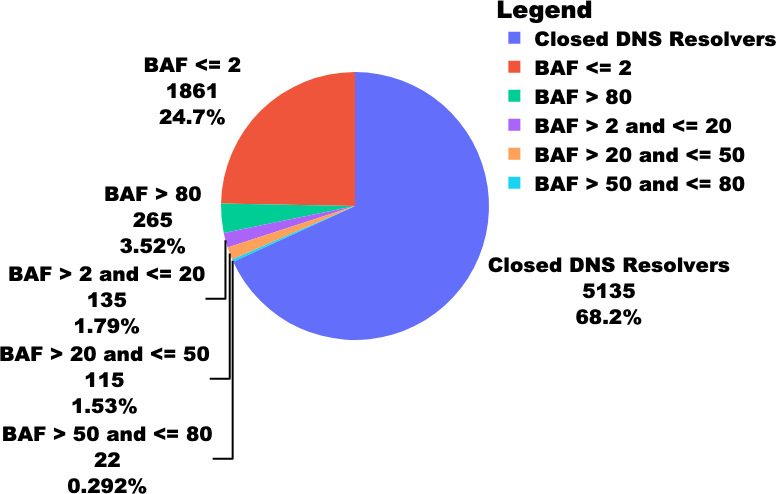
\includegraphics[width=0.48\textwidth]{research paper/plots/dns_sl_piechart_trim.png}
        \caption{DNS BAF distribution.}
        \label{fig:piechart_dns}
\end{figure}

\begin{figure}[t]
        \centering
        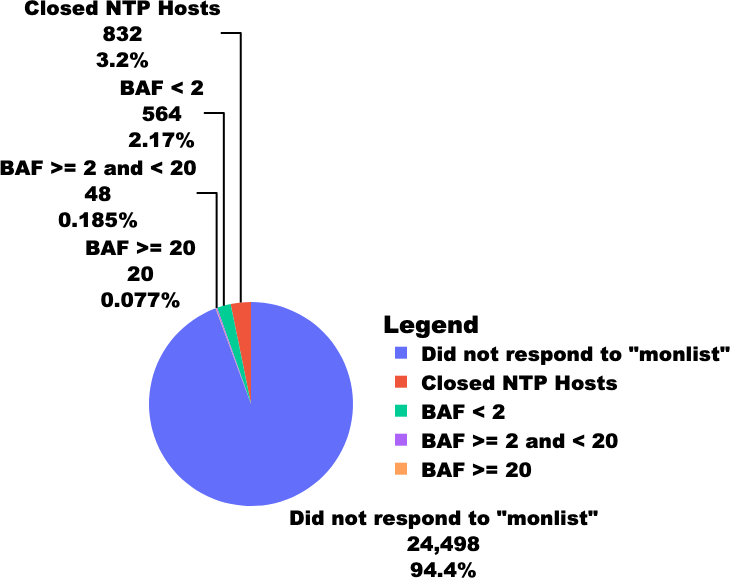
\includegraphics[width=0.48\textwidth]{research paper/plots/ntp_piechart_merged_trim.png}
        \caption{NTP BAF distribution.}
        \label{fig:piechart_ntp}
\end{figure}
    
\begin{figure}[t]
        \centering
        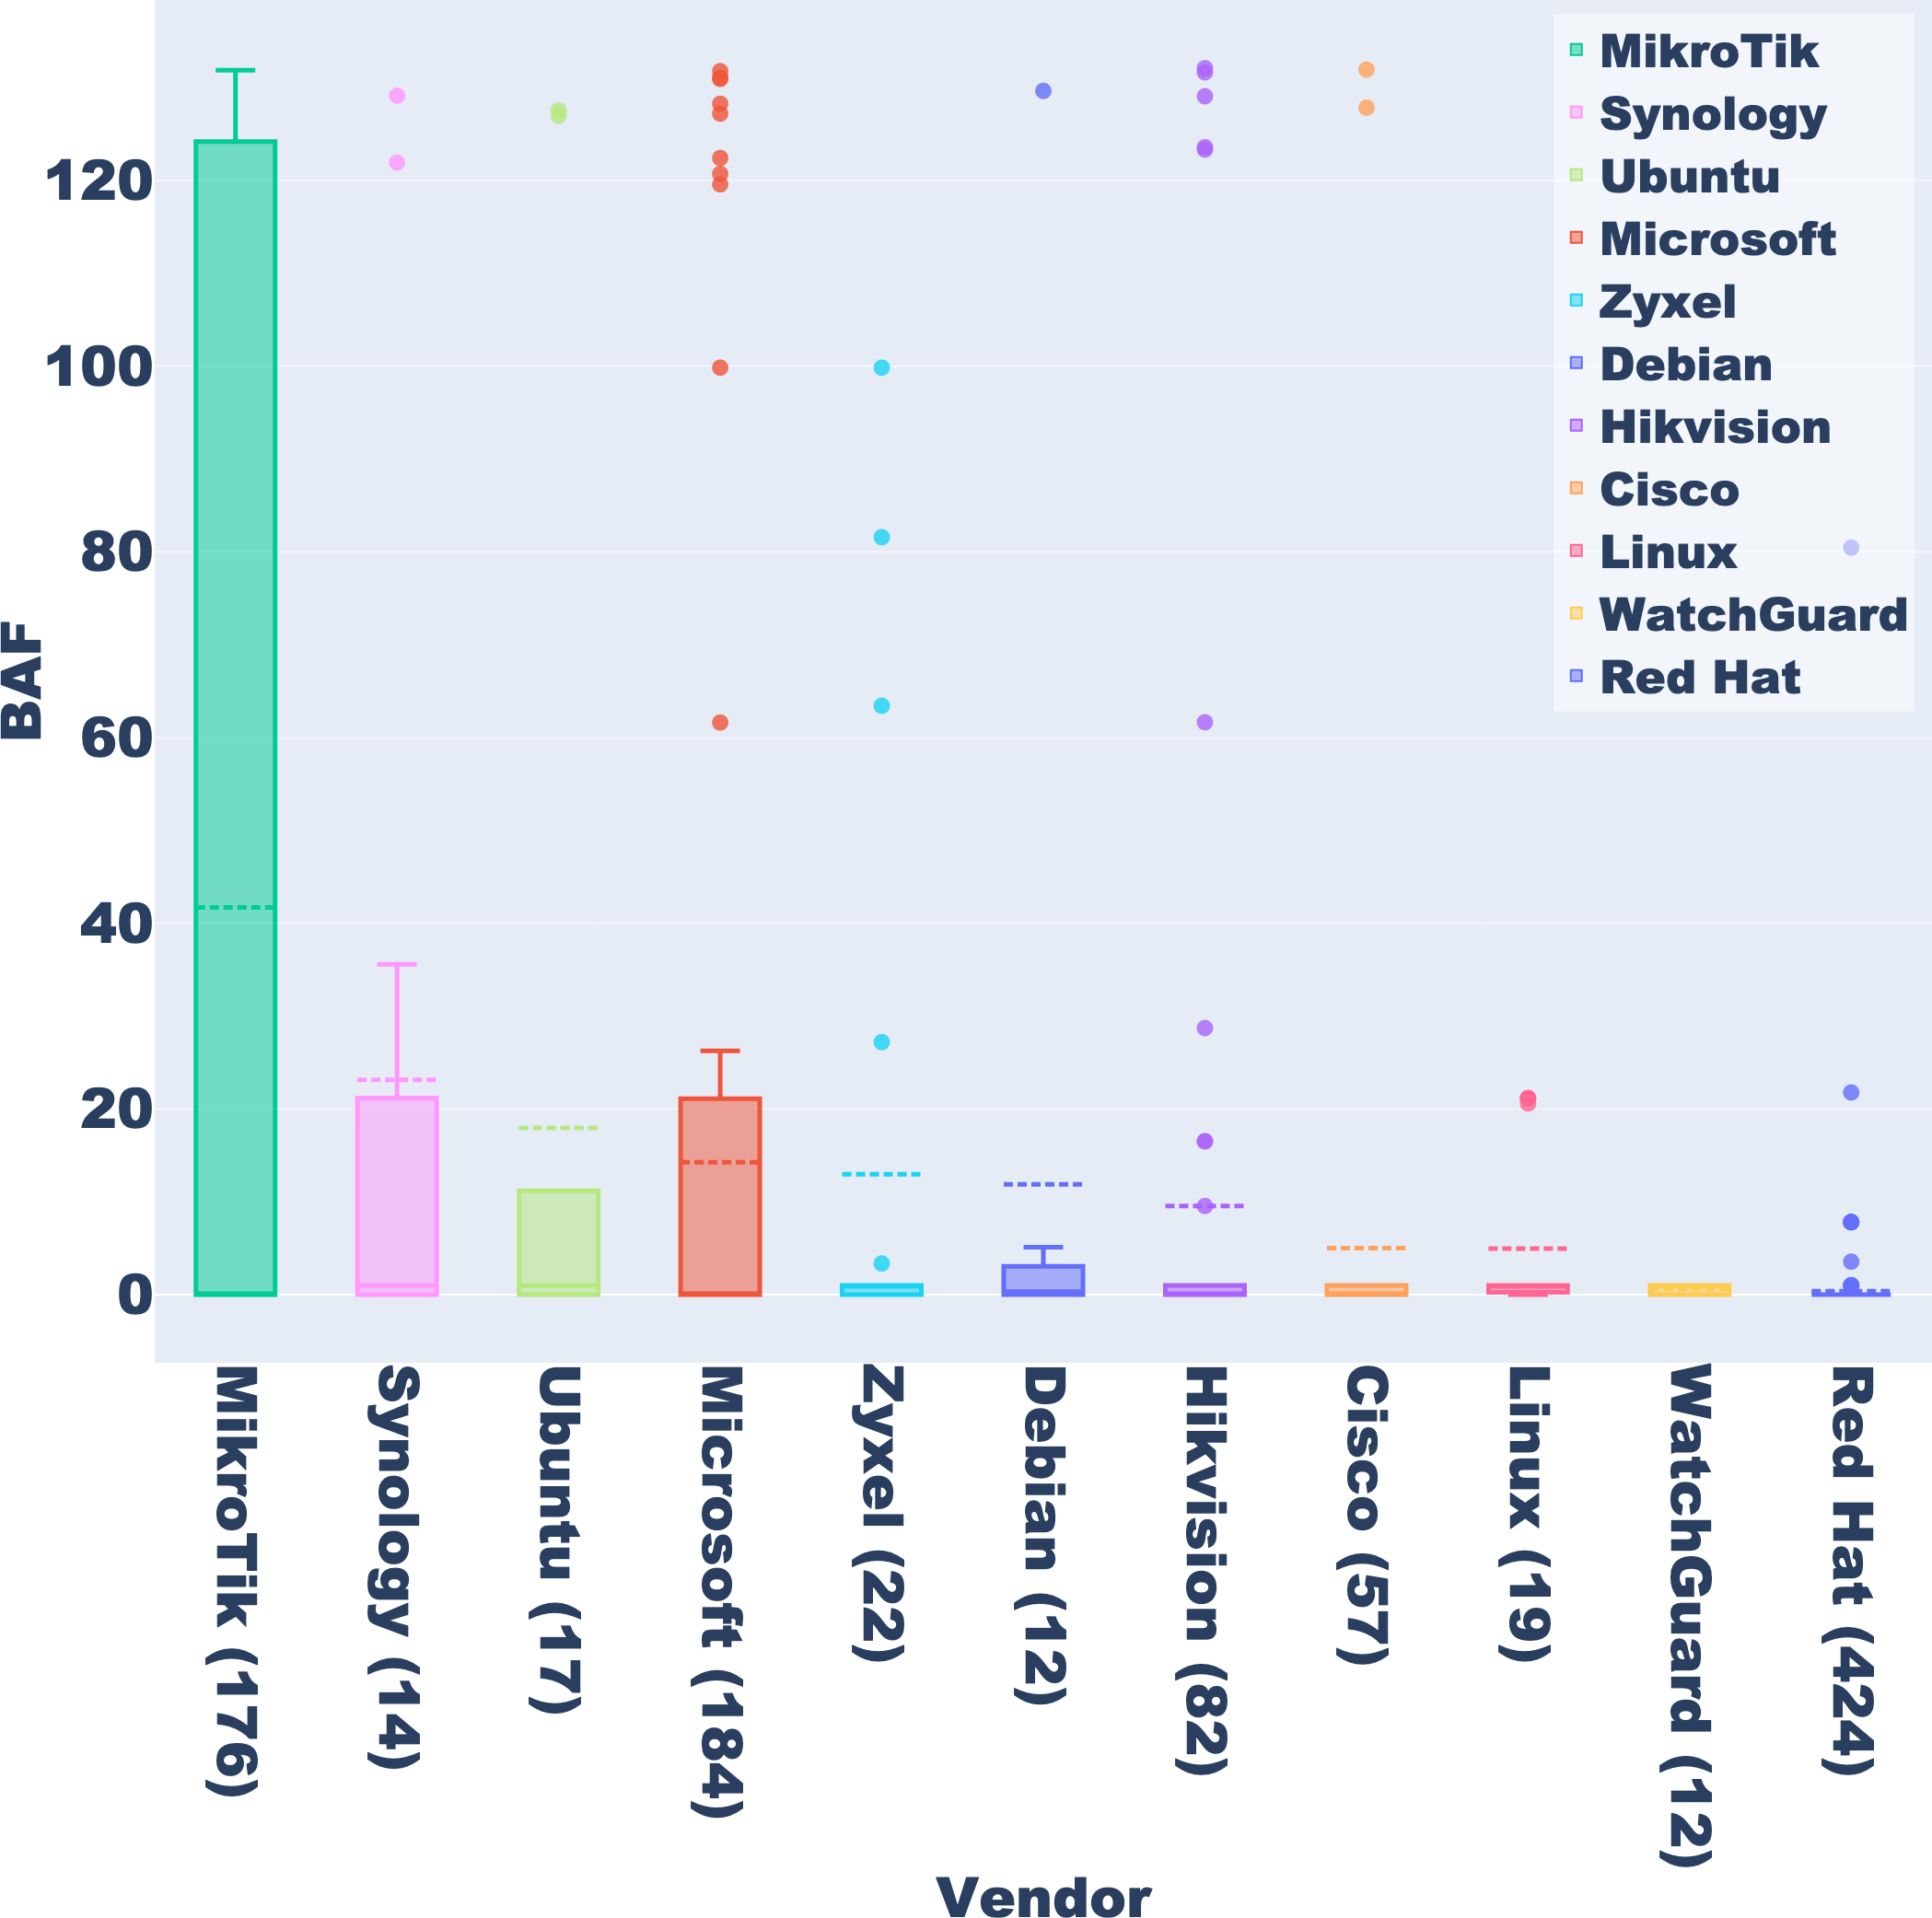
\includegraphics[width=0.48\textwidth]{research paper/plots/SL_vendor_boxplot_restricted_trim.png}
        \caption{Vendor against BAF (DNS).}
        \label{fig:boxplot_vendor}
\end{figure}
    
\begin{figure}[t]
        \centering
        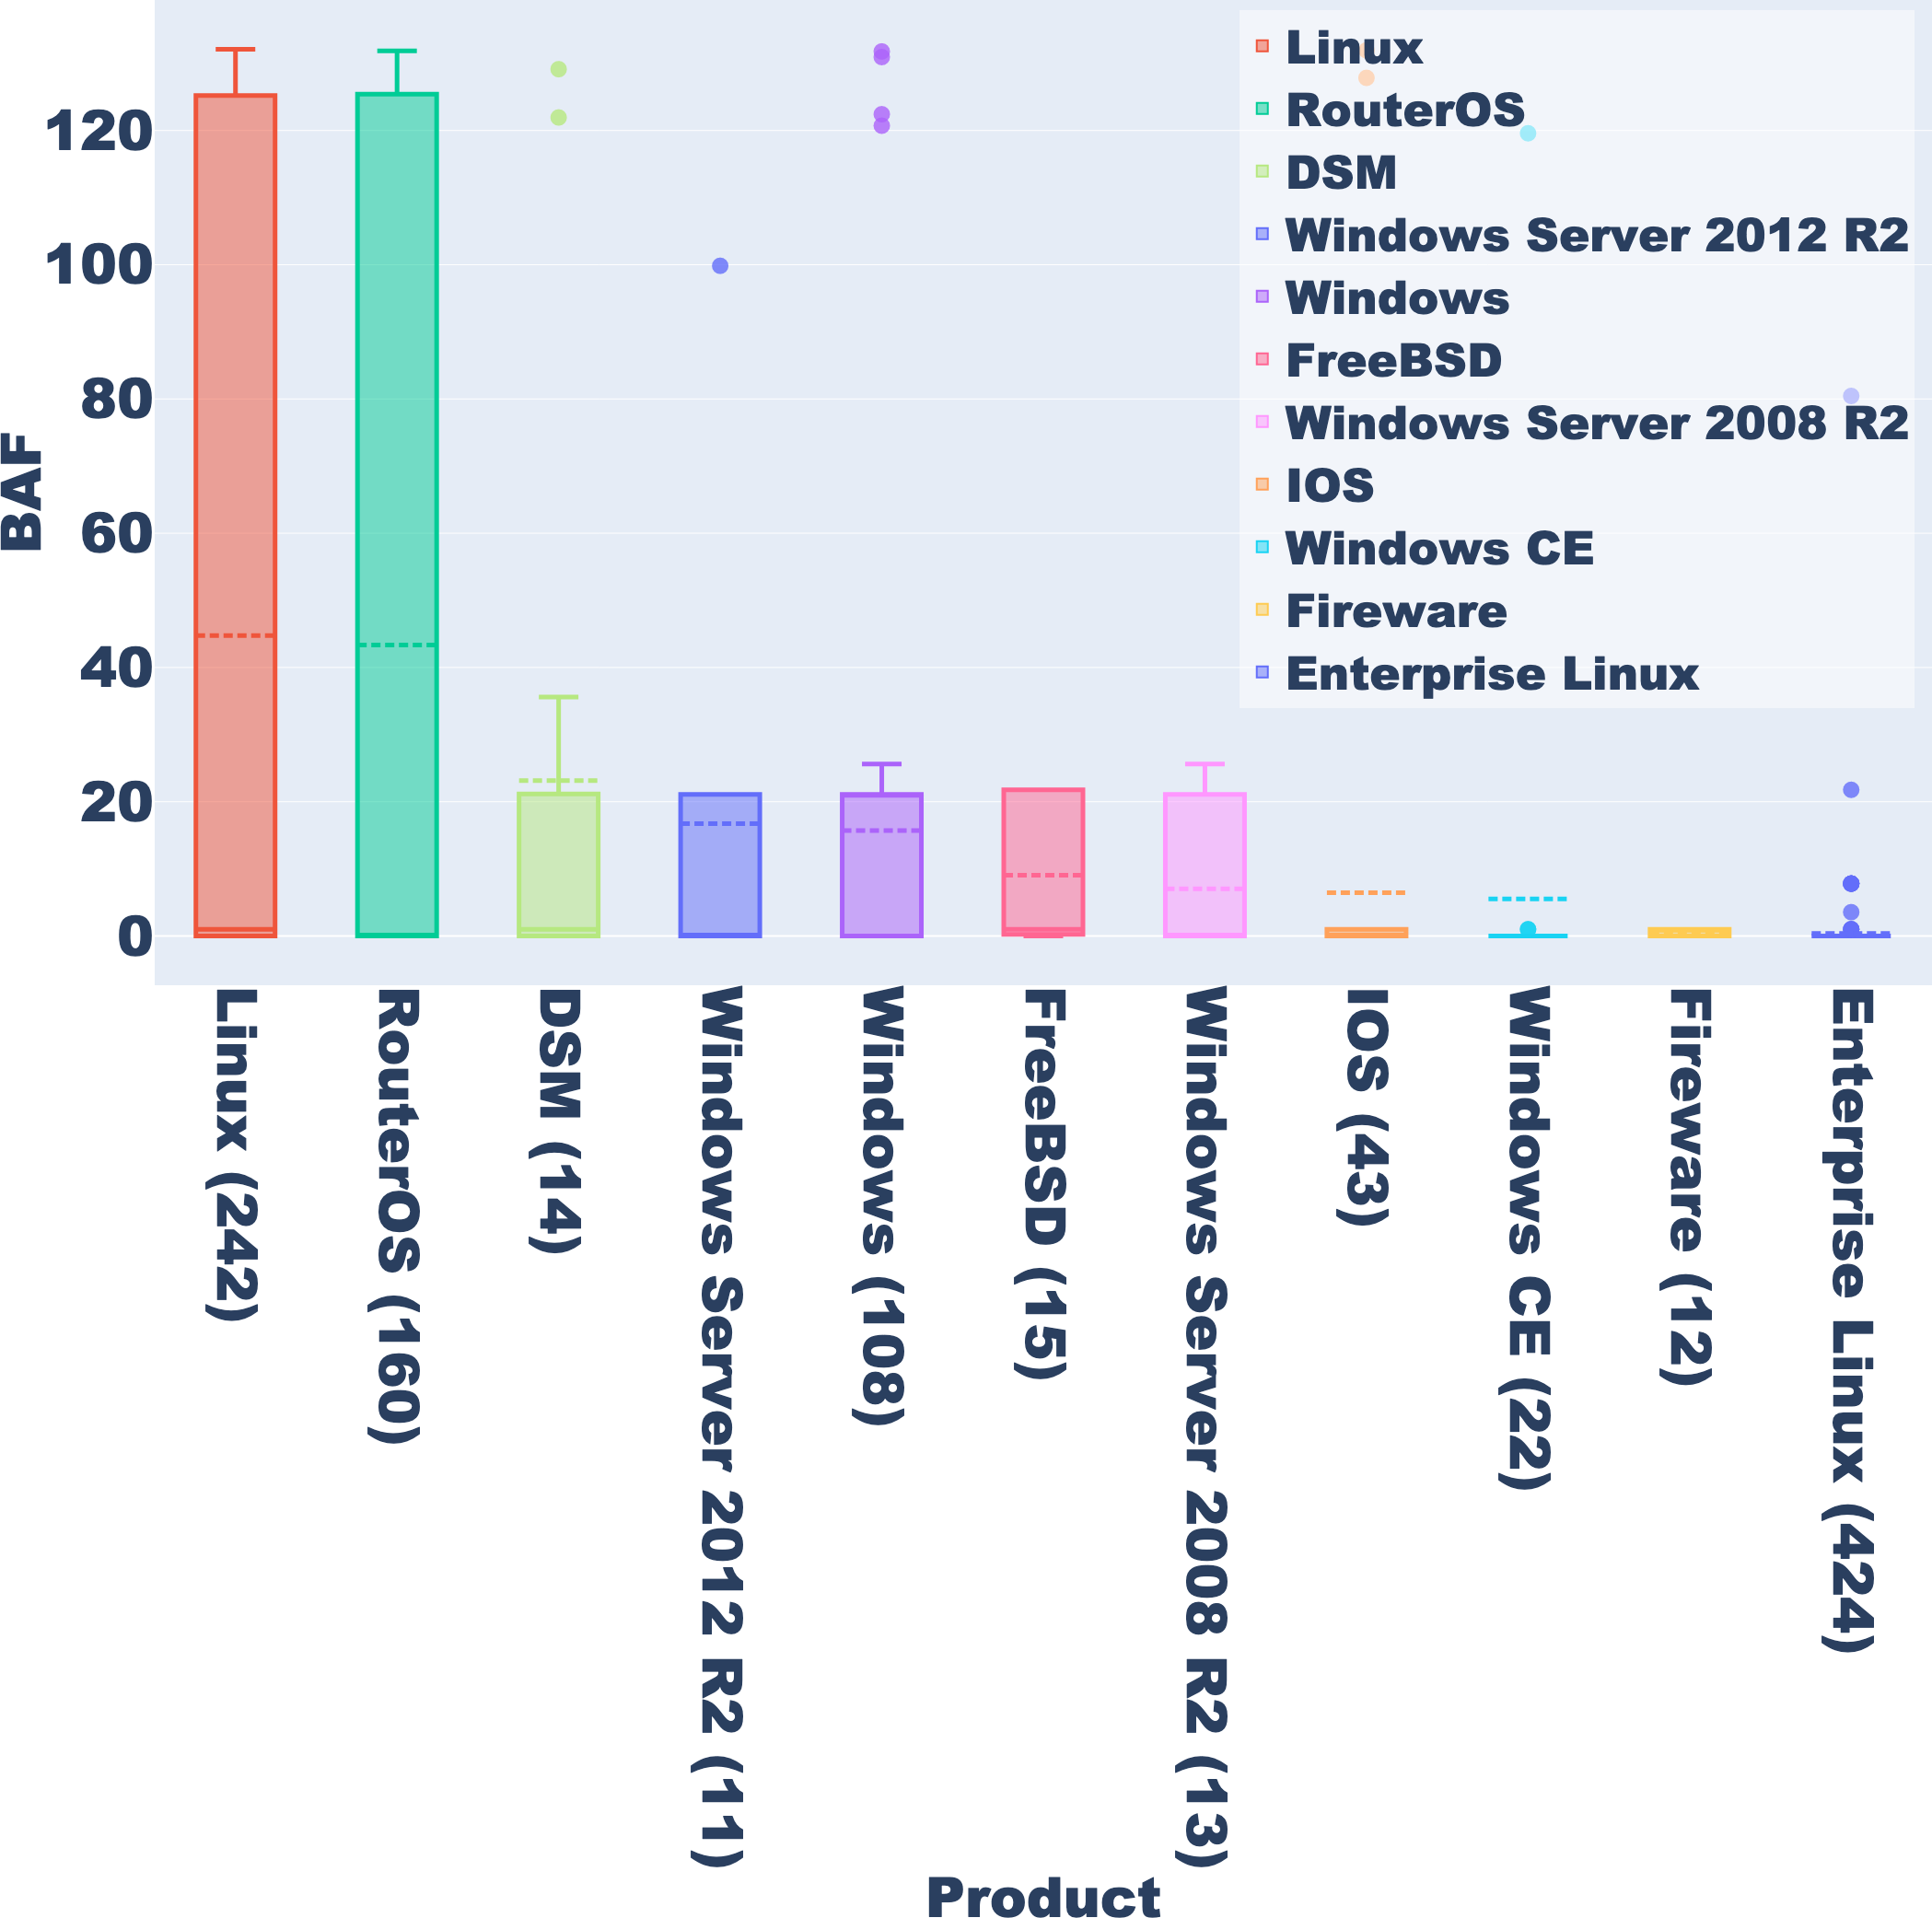
\includegraphics[width=0.48\textwidth]{research paper/plots/SL_product_boxplot_restricted_trim.png}
        \caption{Product against BAF (DNS).}
        \label{fig:boxplot_product}
\end{figure}
    % \caption{Piecharts for DNS and NTP and boxplots for DNS against product and vendor information.}
    % \label{fig:boxplots_piecharts}

\section{Piecharts and Boxplots}
\label{appendix:piecharts_boxplots}



The distribution of DNS hosts according to their BAF is shown in Fig.~\ref{fig:piechart_dns}. Most hosts are closed (68.2\%); however, quite a large amount of DNS hosts (265) achieve a BAF $\geq$ 80. A similar visualisation for NTP is shown in Fig.~\ref{fig:piechart_ntp}. Most NTP servers (94.4\%) did not respond to the ``monlist'' private Mode query for NTP. A few servers are closed (3.2\%), which was expected to ensure accurate and synchronised timekeeping across different devices and networks. Also, a tiny number (20) achieved a BAF $\geq 20$.  

The BAF distribution is depicted in a boxplot from the DNS hosts, whose vendor information we know, in Fig.~\ref{fig:boxplot_vendor}. Red Hat hosts are secure, almost all achieving a BAF of 0. In contrast, MikroTik servers reach the largest BAFs and some Microsoft and Hikvision outlier servers. Furthermore, the product (operating system) boxplot shown in Fig.~\ref{fig:boxplot_product} also shows that servers running RouterOS (from MikroTik) and Linux achieve the highest BAF. Unlike this, Enterprise Linux hosts (from Red Hat) are secure, achieving very small BAFs. Note that there is a high correlation between Fig.~\ref{fig:boxplot_vendor} and Fig.~\ref{fig:boxplot_product} in the sense that, for instance, all the RedHat hosts are running Enterprise Linux or all Synology hosts are running DSM~\cite{dsm}.


\section{Heatmaps}
\label{appendix:heatmaps}

The heatmaps from above compare pairs of factors, and each cell contains the median BAF attained per that respective group. The percentage of the feature on the x-axis is also displayed in parentheses. The total number of servers from certain features is displayed on the left and top borders for the y-axis and x-axis features. Fig.~\ref{fig:heatmap_version_product} shows that, interestingly, servers that get a high BAF that use the MikroTik implementation are not the ones that run Router OS as their operating system. The ones that obtain a high BAF are servers that run DSM (DiskStation Manager - from Synology) and Linux. Similarly, the groups that get the highest BAF in Fig.~\ref{fig:heatmap_buffer_product} are the ones that advertise a Buffer Size of 4,096.

\begin{figure}[t]
    \centering
    \begin{minipage}[t]{0.45\textwidth}
        \centering
        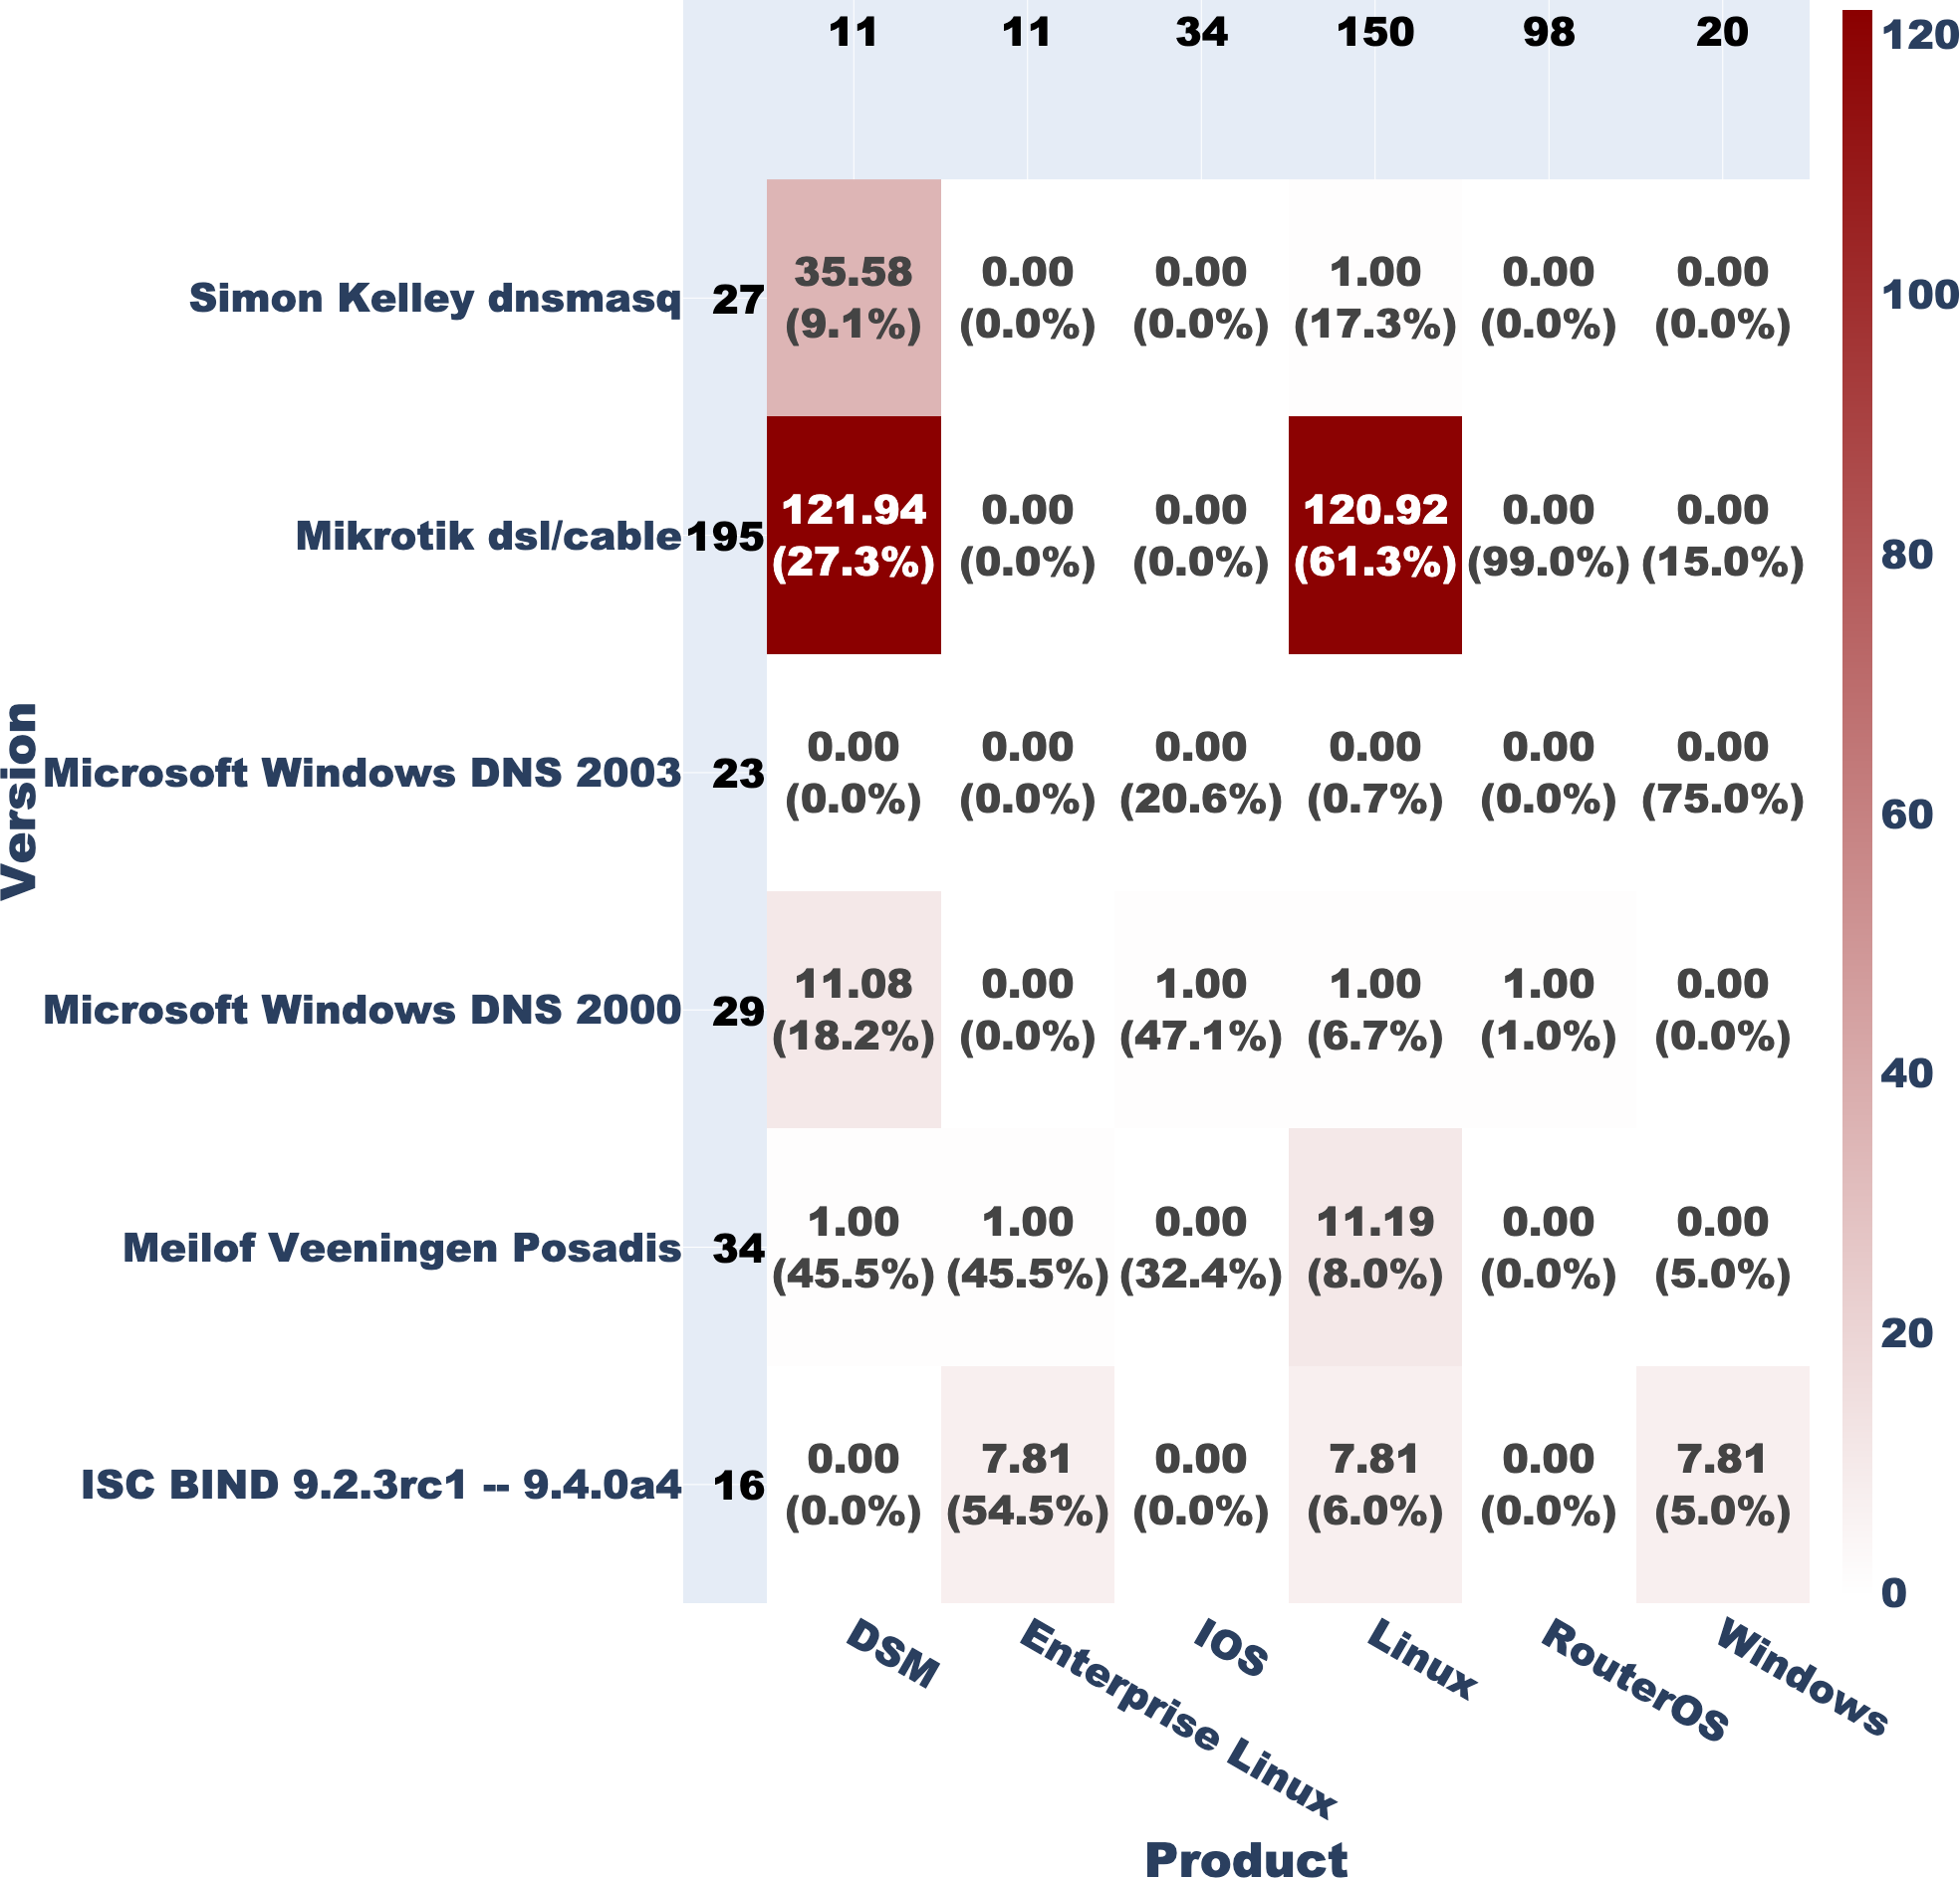
\includegraphics[width=\textwidth]{research paper/plots/filtered_Version_vs_Product_trim.png}
        \caption{Version against Product.}
        \label{fig:heatmap_version_product}
    \end{minipage}
    \hfill
    \begin{minipage}[t]{0.45\textwidth}
        \centering
        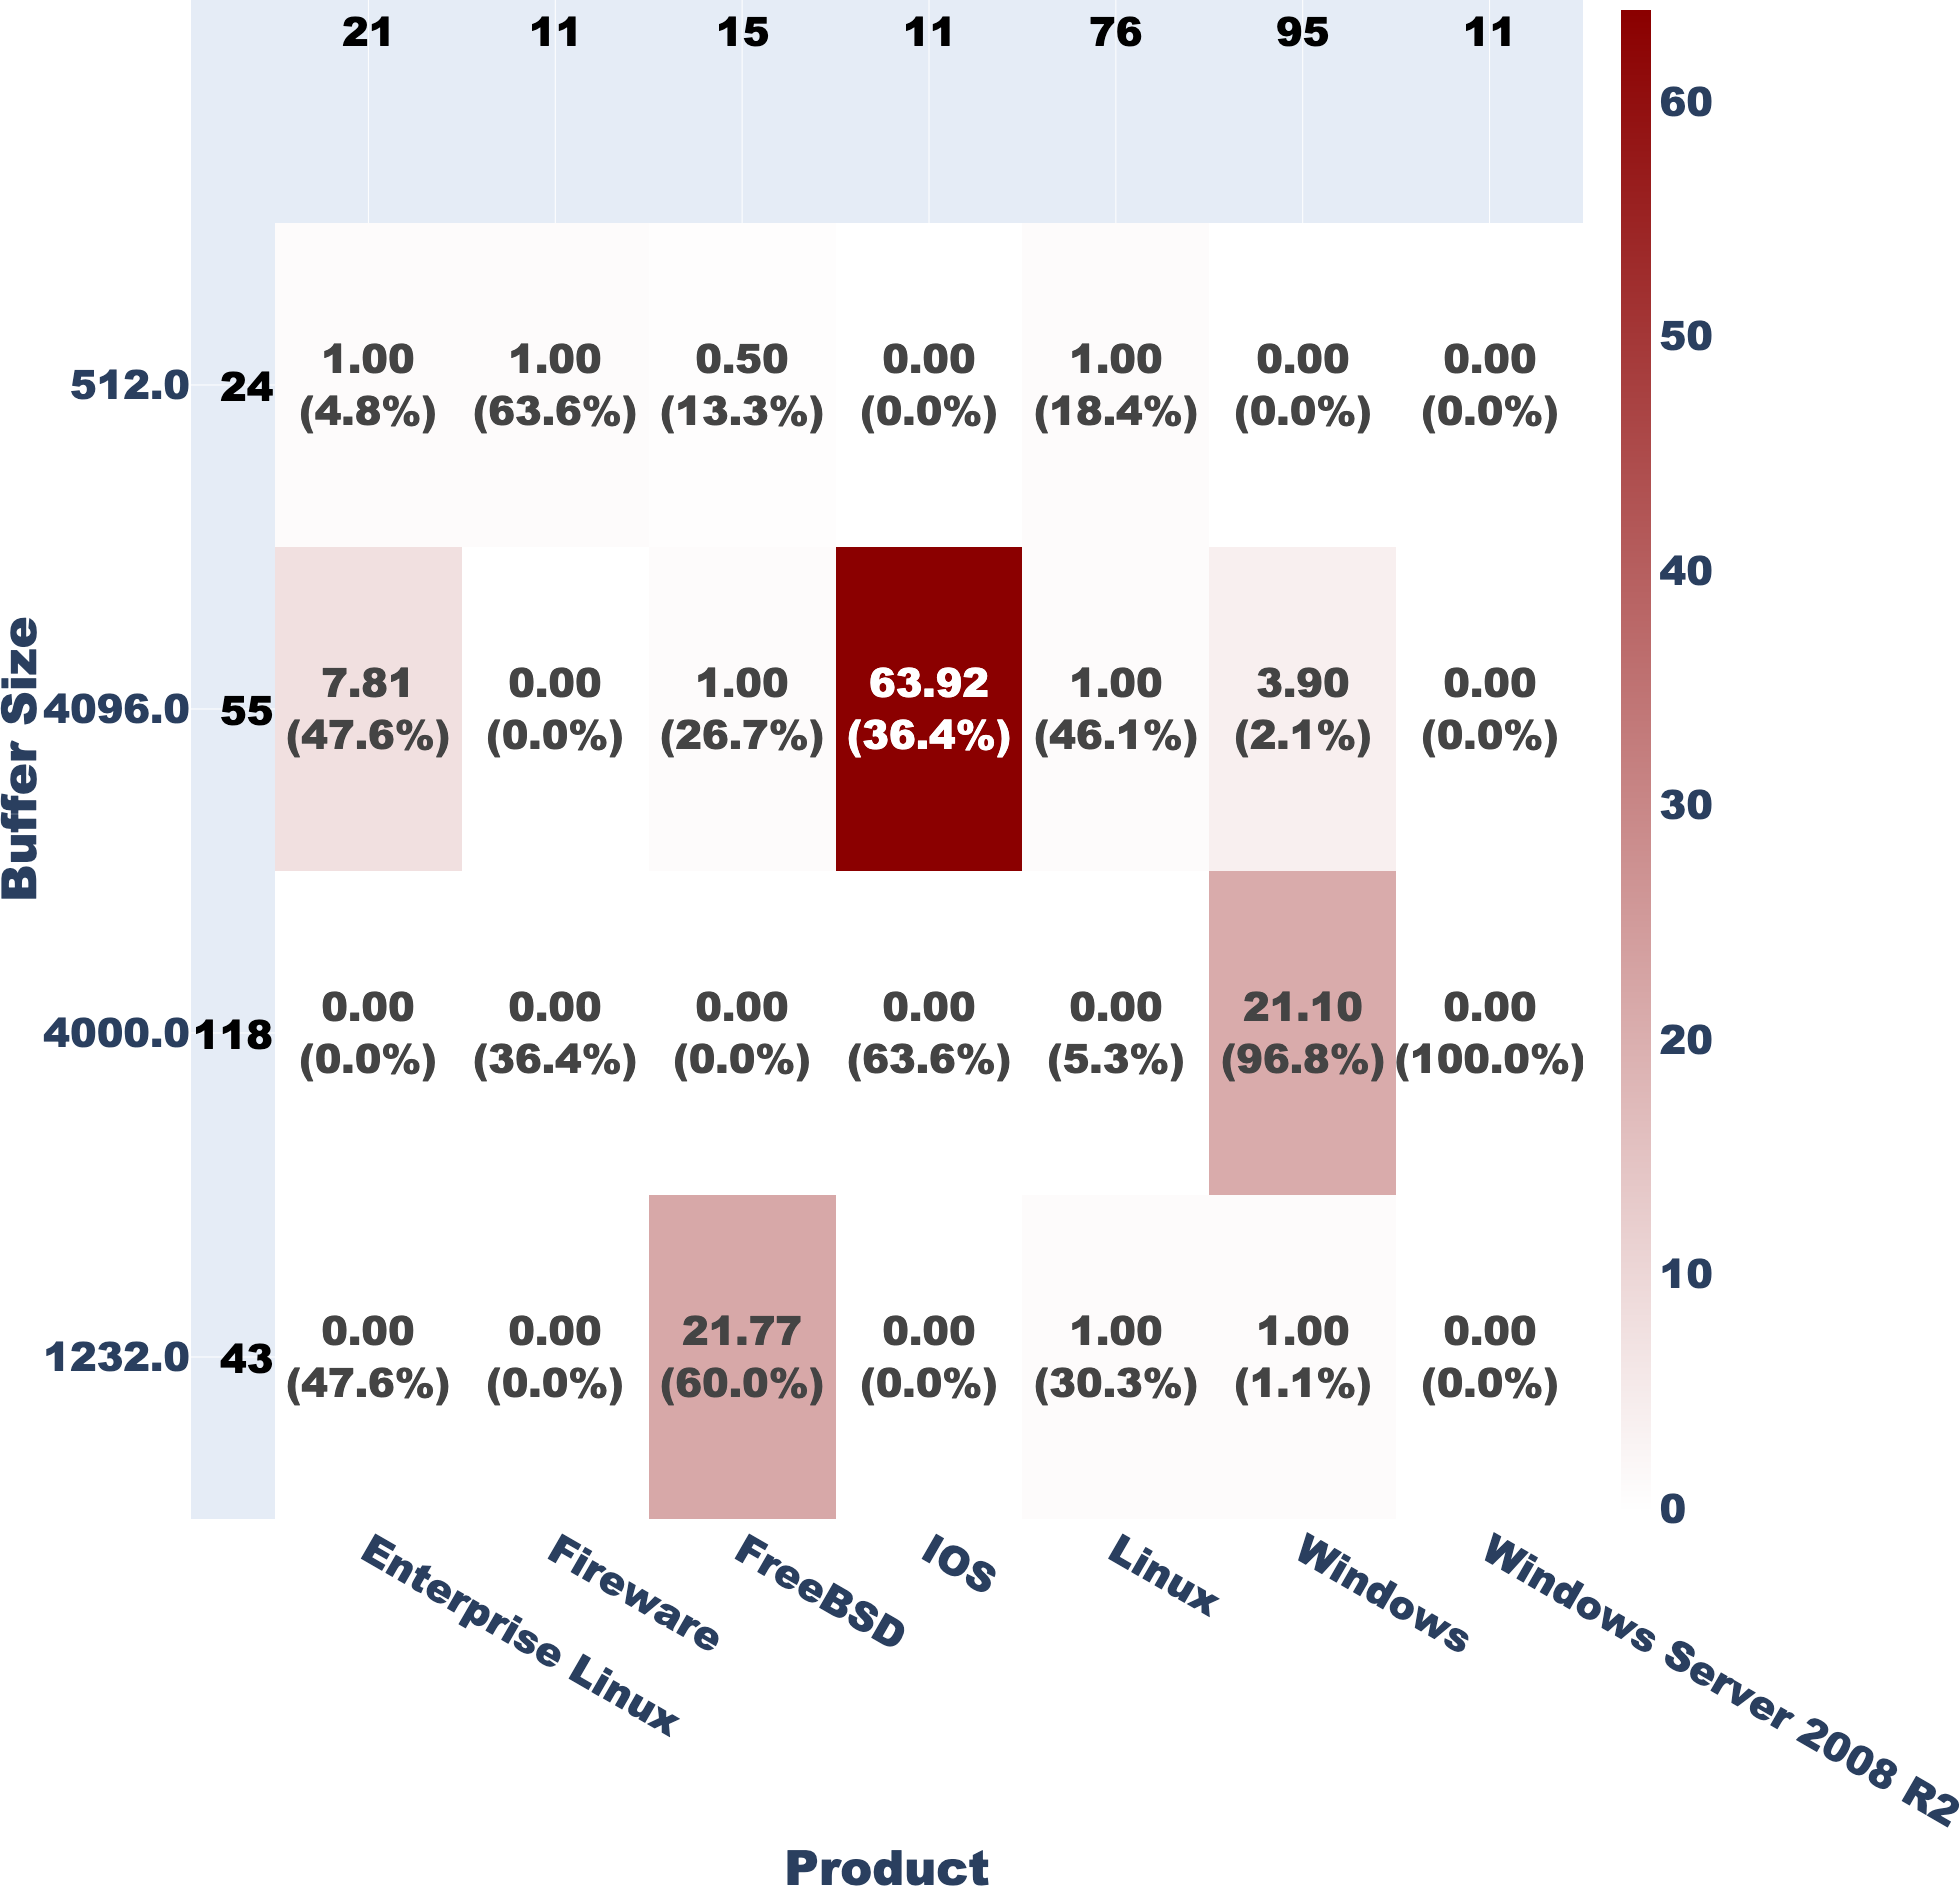
\includegraphics[width=\textwidth]{research paper/plots/filtered_Buffer Size_vs_Product_trim.png}
        \caption{Buffer Size against Product.}
        \label{fig:heatmap_buffer_product}
    \end{minipage}
\end{figure}


\section{Loopy attacks}
\label{appendix:loopy_attacks}
Below is a brief overview of the methodology created by~\cite{cispa-loopy} to find server pairs that are vulnerable to looping attacks. 

\looseness=-1 \textbf{Step 1.} In the first stage discovery packets are sent to all the servers go gather a complete set of responses. These could serve as the entry point to a traffic loop.  

\looseness=-1 \textbf{Step 2.} Since there could be many distinct responses (depending on the number of hosts), the second stage clusters the responses based on their semantics. Insignificant syntactic differences, such as the transaction ID (TXID), are ignored since they cannot influence a DNS response. In the end, several clusters will hold semantically equivalent responses. 

\looseness=-1 \textbf{Step 3.} With a similar reasoning as the second stage, in the third stage, random responses are sampled from each of the clusters. These will be the set of probes that will be sent again to each server. Sending all the initial responses to all the servers would have been both infeasible, due to the large number of initial responses, but also ineffective, since several packets from the same cluster are expected to have the same behaviour, and in turn, should themselves lead to the same response. The responses after this third stage also end up being clustered in the same way as the second stage.  

\looseness=-1 \textbf{Step 4.} With the information gathered in the third step, a loop graph can be formed. In this graph edges represent servers that reply to an input from one cluster with a response from the same or another cluster. Following this, a DFS is ran to find cycles with a length of at most 4.

\looseness=-1 \looseness=-1 \textbf{Step 5.} In the last stage, the loops that were identified previously are formally verified with a proxy. The proxy sits in between the two servers that are being tested and it forwards messages between the two. Once the proxy has forwarded enough messages, the two servers are validated as a loop pair. As this step required setting up a proxy, we have skipped it.

% \clearpage






% \section{Some further guidelines that go without saying (right?)}

% \begin{itemize}
% \item Read the manual for the Research Project. (See e.g.\ the instructions on the maximum length: less is more!)
% \end{itemize}

% \subsection{Reference use}
% \begin{itemize}
% \item use a system for generating the bibliographic information automatically from your database, e.g., use BibTex and/or Mendeley, EndNote, Papers, or \ldots
% \item all ideas, fragments, figures and data that have been quoted from other work have correct references
% \item literal quotations have quotation marks and page numbers
% \item paraphrases are not too close to the original
% \item the references and bibliography meet the requirements
% \item every reference in the text corresponds to an item in the bibliography and vice versa
% \end{itemize}

% \subsection{Structure}
% Paragraphs
% \begin{itemize}
% \item are well-constructed
% \item are not too long: each paragraph discusses one topic
% \item start with clear topic sentences
% \item are divided into a clear paragraph structure
% \item there is a clear line of argumentation from research question to conclusions
% \item scientific literature is reviewed critically
% \end{itemize}

% \subsection{Style}
% \begin{itemize}
% \item correct use of English: understandable, no spelling errors, acceptable grammar, no lexical mistakes 
% \item the style used is objective
% \item clarity: sentences are not too complicated (not too long), there is no ambiguity
% \item attractiveness: sentence length is varied, active voice and passive voice are mixed
% \end{itemize}

% \subsection{Tables and figures}
% \begin{itemize}
% \item all have a number and a caption
% \item all are referred to at least once in the text
% \item if copied, they contain a reference
% \item can be interpreted on their own (e.g. by means of a legend)
% \end{itemize}


\bibliographystyle{plain}
\bibliography{references}

A rule of thumb for dealing with the literature is the following: scan about 10--20 contributions: read title, abstract, part of introduction and conclusions; categorize contribution; some of these are studied in more depth: completely read about 5 conference papers or equivalent (summarize contribution in own words); of which studied in-depth about 2 conference papers (the student is able to explain in detail and criticize contributions). This may result in 5--20 references, possibly even more if the project is a literature study.

\end{document}
